% figs.tex —— 由 ch2/make_figs.py 產生，請勿手動修改。
% 重新產生：python ch2/make_figs.py（第 2 章，動畫 W201–W212）

\newcommand{\TwoTabLegendre}{%
\begin{tabular}{@{}clccc@{}}
\toprule
$n$ & $P_n(x)$ & $\int_{-1}^1P_n\,dx$ & $\int_{-1}^1P_n^2\,dx$ & $\frac{2}{2n+1}$\\
\midrule
0 & $1$ & $2$ & $2$ & $2$\\
1 & $x$ & $0$ & $\tfrac{2}{3}$ & $\tfrac{2}{3}$\\
2 & $\tfrac{3}{2}x^{2}-\tfrac{1}{2}$ & $0$ & $\tfrac{2}{5}$ & $\tfrac{2}{5}$\\
3 & $\tfrac{5}{2}x^{3}-\tfrac{3}{2}x$ & $0$ & $\tfrac{2}{7}$ & $\tfrac{2}{7}$\\
4 & $\tfrac{35}{8}x^{4}-\tfrac{15}{4}x^{2}+\tfrac{3}{8}$ & $0$ & $\tfrac{2}{9}$ & $\tfrac{2}{9}$\\
5 & $\tfrac{63}{8}x^{5}-\tfrac{35}{4}x^{3}+\tfrac{15}{8}x$ & $0$ & $\tfrac{2}{11}$ & $\tfrac{2}{11}$\\
\bottomrule
\end{tabular}}

\newcommand{\TwoTabGrand}{%
\begin{tabular}{@{}ccccccc@{}}
\toprule
$N$ & 0 & 1 & 2 & 3 & 4 & 5\\
\midrule
$Z(N)=2^N/N!$ & $1$ & $2$ & $2$ & $\tfrac{4}{3}$ & $\tfrac{2}{3}$ & $\tfrac{4}{15}$\\
$Z(N)z^N/Q$（$z=1$）& 0.1353 & 0.2707 & 0.2707 & 0.1804 & 0.0902 & 0.0361\\
\bottomrule
\end{tabular}}

\newcommand{\TwoFigMortal}{%
\begin{tikzpicture}[x=0.36cm,y=0.012cm,>=Stealth]
\draw[->] (-0.8,0) -- (21.2,0) node[right,font=\scriptsize] {$n$};
\draw[->] (-0.8,0) -- (-0.8,240) node[above,font=\scriptsize] {人數};
\fill[cBar!55] (-0.38,0) rectangle (0.38,214);
\fill[cBar!55] (0.62,0) rectangle (1.38,167);
\fill[cBar!55] (1.62,0) rectangle (2.38,156);
\fill[cBar!55] (2.62,0) rectangle (3.38,138);
\fill[cBar!55] (3.62,0) rectangle (4.38,119);
\fill[cBar!55] (4.62,0) rectangle (5.38,123);
\fill[cBar!55] (5.62,0) rectangle (6.38,98);
\fill[cBar!55] (6.62,0) rectangle (7.38,94);
\fill[cBar!55] (7.62,0) rectangle (8.38,88);
\fill[cBar!55] (8.62,0) rectangle (9.38,71);
\fill[cBar!55] (9.62,0) rectangle (10.38,74);
\fill[cBar!55] (10.62,0) rectangle (11.38,58);
\fill[cBar!55] (11.62,0) rectangle (12.38,63);
\fill[cBar!55] (12.62,0) rectangle (13.38,54);
\fill[cBar!55] (13.62,0) rectangle (14.38,59);
\fill[cBar!55] (14.62,0) rectangle (15.38,44);
\fill[cBar!55] (15.62,0) rectangle (16.38,36);
\fill[cBar!55] (16.62,0) rectangle (17.38,36);
\fill[cBar!55] (17.62,0) rectangle (18.38,28);
\fill[cBar!55] (18.62,0) rectangle (19.38,30);
\fill[cBar!55] (19.62,0) rectangle (20.38,26);
\draw[cGauss,thick] plot coordinates {(0,200.00) (1,180.00) (2,162.00) (3,145.80) (4,131.22) (5,118.10) (6,106.29) (7,95.66) (8,86.09) (9,77.48) (10,69.74) (11,62.76) (12,56.49) (13,50.84) (14,45.75) (15,41.18) (16,37.06) (17,33.35) (18,30.02) (19,27.02) (20,24.32)};
\foreach \k in {0,5,10,15,20} \node[below,font=\scriptsize] at (\k,0) {\k};
\foreach \v in {100,200} {\draw (-0.95,\v) -- (-0.65,\v); \node[left,font=\scriptsize] at (-0.9,\v) {\v};}
\node[right,font=\scriptsize,cGauss] at (6,200) {理論 $2000\times0.1\times0.9^n$};
\end{tikzpicture}}

\newcommand{\TwoFigCountGrid}{%
\begin{tikzpicture}[>=Stealth]
\begin{scope}[shift={(0,0)}]
\draw[gray!40] (-1.5*0.9,-1.5*0.9) grid[step=0.9] (1.5*0.9,1.5*0.9);
\fill[gray] (-0.9,0.0) circle (2.6pt);
\draw[->,gray!70!black,thick] (-0.765,0.0) -- (-0.18000000000000002,0.0);
\node[below left,font=\scriptsize] at (-0.9,0.0) {$\vec w_1$};
\fill[gray] (0.0,-0.9) circle (2.6pt);
\draw[->,gray!70!black,thick] (0.0,-0.765) -- (0.0,-0.18000000000000002);
\node[below left,font=\scriptsize] at (0.0,-0.9) {$\vec w_2$};
\fill[gray] (0.9,0.0) circle (2.6pt);
\draw[->,gray!70!black,thick] (0.765,0.0) -- (0.18000000000000002,0.0);
\node[above right,font=\scriptsize] at (0.9,0.0) {$\vec w_3$};
\fill[gray] (0.0,0.9) circle (2.6pt);
\draw[->,gray!70!black,thick] (0.0,0.765) -- (0.0,0.18000000000000002);
\node[above right,font=\scriptsize] at (0.0,0.9) {$\vec w_4$};
\fill (0,0) circle (3pt); \node[below right,font=\scriptsize] at (0,0) {$\vec y$};
\node[font=\small] at (0,-2.0) {(a) 最後一步來自四個鄰居};
\end{scope}
\begin{scope}[shift={(4.2,0)}]
\draw[gray!30] (-2.5*0.5,-2.5*0.5) grid[step=0.5] (2.5*0.5,2.5*0.5);
\node[font=\scriptsize,text=black] at (-1.0,0.0) {1};
\node[font=\scriptsize,text=black] at (-0.5,-0.5) {2};
\node[font=\scriptsize,text=black] at (-0.5,0.5) {2};
\node[font=\scriptsize,text=black] at (0.0,-1.0) {1};
\node[font=\scriptsize,text=cWalk] at (0.0,0.0) {4};
\node[font=\scriptsize,text=black] at (0.0,1.0) {1};
\node[font=\scriptsize,text=black] at (0.5,-0.5) {2};
\node[font=\scriptsize,text=black] at (0.5,0.5) {2};
\node[font=\scriptsize,text=black] at (1.0,0.0) {1};
\node[font=\small] at (0,-1.75) {(b) $N=2$，總和 $16$};
\end{scope}
\begin{scope}[shift={(9.3,0)}]
\draw[gray!30] (-4.5*0.5,-4.5*0.5) grid[step=0.5] (4.5*0.5,4.5*0.5);
\node[font=\scriptsize,text=black] at (-2.0,0.0) {1};
\node[font=\scriptsize,text=black] at (-1.5,-0.5) {4};
\node[font=\scriptsize,text=black] at (-1.5,0.5) {4};
\node[font=\scriptsize,text=black] at (-1.0,-1.0) {6};
\node[font=\scriptsize,text=black] at (-1.0,0.0) {16};
\node[font=\scriptsize,text=black] at (-1.0,1.0) {6};
\node[font=\scriptsize,text=black] at (-0.5,-1.5) {4};
\node[font=\scriptsize,text=black] at (-0.5,-0.5) {24};
\node[font=\scriptsize,text=black] at (-0.5,0.5) {24};
\node[font=\scriptsize,text=black] at (-0.5,1.5) {4};
\node[font=\scriptsize,text=black] at (0.0,-2.0) {1};
\node[font=\scriptsize,text=black] at (0.0,-1.0) {16};
\node[font=\scriptsize,text=cWalk] at (0.0,0.0) {36};
\node[font=\scriptsize,text=black] at (0.0,1.0) {16};
\node[font=\scriptsize,text=black] at (0.0,2.0) {1};
\node[font=\scriptsize,text=black] at (0.5,-1.5) {4};
\node[font=\scriptsize,text=black] at (0.5,-0.5) {24};
\node[font=\scriptsize,text=black] at (0.5,0.5) {24};
\node[font=\scriptsize,text=black] at (0.5,1.5) {4};
\node[font=\scriptsize,text=black] at (1.0,-1.0) {6};
\node[font=\scriptsize,text=black] at (1.0,0.0) {16};
\node[font=\scriptsize,text=black] at (1.0,1.0) {6};
\node[font=\scriptsize,text=black] at (1.5,-0.5) {4};
\node[font=\scriptsize,text=black] at (1.5,0.5) {4};
\node[font=\scriptsize,text=black] at (2.0,0.0) {1};
\node[font=\small] at (0,-2.75) {(c) $N=4$，總和 $256$};
\end{scope}
\end{tikzpicture}}

\newcommand{\TwoTabChi}{%
\begin{tabular}{@{}llcccc@{}}
\toprule
格子 & $\chi(\vec q)$（$a=1$） & $\chi(\vec0)$ & 小 $q$ & 單胞體積 $\Omega$ & 二部圖\\
\midrule
一維 & $2\cos q$ & 2 & $2-q^2$ & 1 & 是\\
正方 & $2(\cos q_x+\cos q_y)$ & 4 & $4-q^2$ & 1 & 是\\
簡單立方 sc & $2(\cos q_x+\cos q_y+\cos q_z)$ & 6 & $6-q^2$ & 1 & 是\\
體心立方 bcc & $8\cos\frac{q_x}{\sqrt3}\cos\frac{q_y}{\sqrt3}\cos\frac{q_z}{\sqrt3}$ & 8 & $8-\frac43q^2$ & 0.7698 & 是\\
面心立方 fcc & $4\big[\cos\frac{q_x}{\sqrt2}\cos\frac{q_y}{\sqrt2}+\cdots\big]$ & 12 & $12-2q^2$ & 0.7071 & 否\\
\bottomrule
\end{tabular}}

\newcommand{\TwoTabReturns}{%
{\small\setlength{\tabcolsep}{3.2pt}\begin{tabular}{@{}lrrrrrrrrrrr@{}}
\toprule
$N$ & 0 & 1 & 2 & 3 & 4 & 5 & 6 & 7 & 8 & 9 & 10\\
\midrule
一維 $\binom{N}{N/2}$ & 1 & 0 & 2 & 0 & 6 & 0 & 20 & 0 & 70 & 0 & 252\\
正方 & 1 & 0 & 4 & 0 & 36 & 0 & 400 & 0 & 4\,900 & 0 & 63\,504\\
sc & 1 & 0 & 6 & 0 & 90 & 0 & 1\,860 & 0 & 44\,730 & 0 & 1\,172\,556\\
bcc & 1 & 0 & 8 & 0 & 216 & 0 & 8\,000 & 0 & 343\,000 & 0 & 16\,003\,008\\
fcc & 1 & 0 & 12 & 48 & 540 & 4\,320 & 42\,240 & 403\,200 & 4\,038\,300 & 40\,958\,400 & 423\,550\,512\\
\bottomrule
\end{tabular}}}

\newcommand{\TwoFigHeat}{%
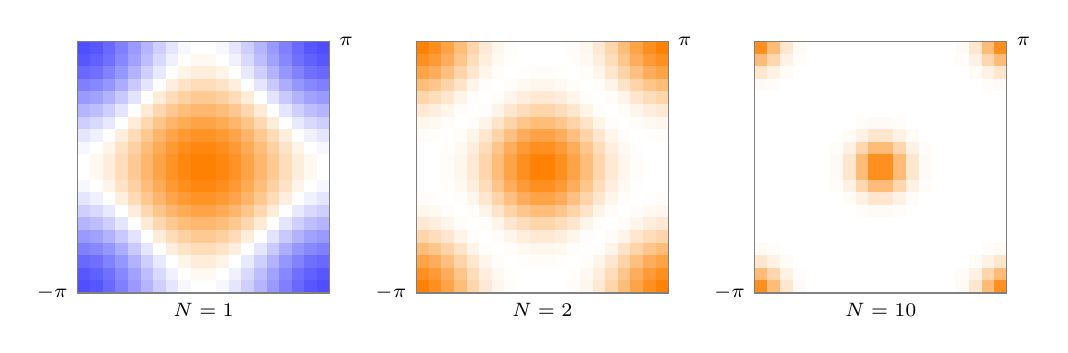
\begin{tikzpicture}
\begin{scope}[shift={(0.0,0)}]
\fill[blue!69!white] (0.000,0.000) rectangle (0.160,0.160);
\fill[blue!66!white] (0.160,0.000) rectangle (0.320,0.160);
\fill[blue!59!white] (0.320,0.000) rectangle (0.480,0.160);
\fill[blue!50!white] (0.480,0.000) rectangle (0.640,0.160);
\fill[blue!40!white] (0.640,0.000) rectangle (0.800,0.160);
\fill[blue!29!white] (0.800,0.000) rectangle (0.960,0.160);
\fill[blue!19!white] (0.960,0.000) rectangle (1.120,0.160);
\fill[blue!10!white] (1.120,0.000) rectangle (1.280,0.160);
\fill[blue!3!white] (1.280,0.000) rectangle (1.440,0.160);
\fill[orange!0!white] (1.440,0.000) rectangle (1.600,0.160);
\fill[orange!0!white] (1.600,0.000) rectangle (1.760,0.160);
\fill[blue!3!white] (1.760,0.000) rectangle (1.920,0.160);
\fill[blue!10!white] (1.920,0.000) rectangle (2.080,0.160);
\fill[blue!19!white] (2.080,0.000) rectangle (2.240,0.160);
\fill[blue!29!white] (2.240,0.000) rectangle (2.400,0.160);
\fill[blue!40!white] (2.400,0.000) rectangle (2.560,0.160);
\fill[blue!50!white] (2.560,0.000) rectangle (2.720,0.160);
\fill[blue!59!white] (2.720,0.000) rectangle (2.880,0.160);
\fill[blue!66!white] (2.880,0.000) rectangle (3.040,0.160);
\fill[blue!69!white] (3.040,0.000) rectangle (3.200,0.160);
\fill[blue!66!white] (0.000,0.160) rectangle (0.160,0.320);
\fill[blue!62!white] (0.160,0.160) rectangle (0.320,0.320);
\fill[blue!56!white] (0.320,0.160) rectangle (0.480,0.320);
\fill[blue!47!white] (0.480,0.160) rectangle (0.640,0.320);
\fill[blue!37!white] (0.640,0.160) rectangle (0.800,0.320);
\fill[blue!26!white] (0.800,0.160) rectangle (0.960,0.320);
\fill[blue!15!white] (0.960,0.160) rectangle (1.120,0.320);
\fill[blue!6!white] (1.120,0.160) rectangle (1.280,0.320);
\fill[orange!0!white] (1.280,0.160) rectangle (1.440,0.320);
\fill[orange!5!white] (1.440,0.160) rectangle (1.600,0.320);
\fill[orange!5!white] (1.600,0.160) rectangle (1.760,0.320);
\fill[orange!0!white] (1.760,0.160) rectangle (1.920,0.320);
\fill[blue!6!white] (1.920,0.160) rectangle (2.080,0.320);
\fill[blue!15!white] (2.080,0.160) rectangle (2.240,0.320);
\fill[blue!26!white] (2.240,0.160) rectangle (2.400,0.320);
\fill[blue!37!white] (2.400,0.160) rectangle (2.560,0.320);
\fill[blue!47!white] (2.560,0.160) rectangle (2.720,0.320);
\fill[blue!56!white] (2.720,0.160) rectangle (2.880,0.320);
\fill[blue!62!white] (2.880,0.160) rectangle (3.040,0.320);
\fill[blue!66!white] (3.040,0.160) rectangle (3.200,0.320);
\fill[blue!59!white] (0.000,0.320) rectangle (0.160,0.480);
\fill[blue!56!white] (0.160,0.320) rectangle (0.320,0.480);
\fill[blue!49!white] (0.320,0.320) rectangle (0.480,0.480);
\fill[blue!41!white] (0.480,0.320) rectangle (0.640,0.480);
\fill[blue!30!white] (0.640,0.320) rectangle (0.800,0.480);
\fill[blue!19!white] (0.800,0.320) rectangle (0.960,0.480);
\fill[blue!9!white] (0.960,0.320) rectangle (1.120,0.480);
\fill[orange!0!white] (1.120,0.320) rectangle (1.280,0.480);
\fill[orange!9!white] (1.280,0.320) rectangle (1.440,0.480);
\fill[orange!14!white] (1.440,0.320) rectangle (1.600,0.480);
\fill[orange!14!white] (1.600,0.320) rectangle (1.760,0.480);
\fill[orange!9!white] (1.760,0.320) rectangle (1.920,0.480);
\fill[orange!0!white] (1.920,0.320) rectangle (2.080,0.480);
\fill[blue!9!white] (2.080,0.320) rectangle (2.240,0.480);
\fill[blue!19!white] (2.240,0.320) rectangle (2.400,0.480);
\fill[blue!30!white] (2.400,0.320) rectangle (2.560,0.480);
\fill[blue!41!white] (2.560,0.320) rectangle (2.720,0.480);
\fill[blue!49!white] (2.720,0.320) rectangle (2.880,0.480);
\fill[blue!56!white] (2.880,0.320) rectangle (3.040,0.480);
\fill[blue!59!white] (3.040,0.320) rectangle (3.200,0.480);
\fill[blue!50!white] (0.000,0.480) rectangle (0.160,0.640);
\fill[blue!47!white] (0.160,0.480) rectangle (0.320,0.640);
\fill[blue!41!white] (0.320,0.480) rectangle (0.480,0.640);
\fill[blue!32!white] (0.480,0.480) rectangle (0.640,0.640);
\fill[blue!21!white] (0.640,0.480) rectangle (0.800,0.640);
\fill[blue!10!white] (0.800,0.480) rectangle (0.960,0.640);
\fill[orange!0!white] (0.960,0.480) rectangle (1.120,0.640);
\fill[orange!13!white] (1.120,0.480) rectangle (1.280,0.640);
\fill[orange!22!white] (1.280,0.480) rectangle (1.440,0.640);
\fill[orange!27!white] (1.440,0.480) rectangle (1.600,0.640);
\fill[orange!27!white] (1.600,0.480) rectangle (1.760,0.640);
\fill[orange!22!white] (1.760,0.480) rectangle (1.920,0.640);
\fill[orange!13!white] (1.920,0.480) rectangle (2.080,0.640);
\fill[orange!0!white] (2.080,0.480) rectangle (2.240,0.640);
\fill[blue!10!white] (2.240,0.480) rectangle (2.400,0.640);
\fill[blue!21!white] (2.400,0.480) rectangle (2.560,0.640);
\fill[blue!32!white] (2.560,0.480) rectangle (2.720,0.640);
\fill[blue!41!white] (2.720,0.480) rectangle (2.880,0.640);
\fill[blue!47!white] (2.880,0.480) rectangle (3.040,0.640);
\fill[blue!50!white] (3.040,0.480) rectangle (3.200,0.640);
\fill[blue!40!white] (0.000,0.640) rectangle (0.160,0.800);
\fill[blue!37!white] (0.160,0.640) rectangle (0.320,0.800);
\fill[blue!30!white] (0.320,0.640) rectangle (0.480,0.800);
\fill[blue!21!white] (0.480,0.640) rectangle (0.640,0.800);
\fill[blue!11!white] (0.640,0.640) rectangle (0.800,0.800);
\fill[blue!0!white] (0.800,0.640) rectangle (0.960,0.800);
\fill[orange!15!white] (0.960,0.640) rectangle (1.120,0.800);
\fill[orange!28!white] (1.120,0.640) rectangle (1.280,0.800);
\fill[orange!37!white] (1.280,0.640) rectangle (1.440,0.800);
\fill[orange!42!white] (1.440,0.640) rectangle (1.600,0.800);
\fill[orange!42!white] (1.600,0.640) rectangle (1.760,0.800);
\fill[orange!37!white] (1.760,0.640) rectangle (1.920,0.800);
\fill[orange!28!white] (1.920,0.640) rectangle (2.080,0.800);
\fill[orange!15!white] (2.080,0.640) rectangle (2.240,0.800);
\fill[orange!0!white] (2.240,0.640) rectangle (2.400,0.800);
\fill[blue!11!white] (2.400,0.640) rectangle (2.560,0.800);
\fill[blue!21!white] (2.560,0.640) rectangle (2.720,0.800);
\fill[blue!30!white] (2.720,0.640) rectangle (2.880,0.800);
\fill[blue!37!white] (2.880,0.640) rectangle (3.040,0.800);
\fill[blue!40!white] (3.040,0.640) rectangle (3.200,0.800);
\fill[blue!29!white] (0.000,0.800) rectangle (0.160,0.960);
\fill[blue!26!white] (0.160,0.800) rectangle (0.320,0.960);
\fill[blue!19!white] (0.320,0.800) rectangle (0.480,0.960);
\fill[blue!10!white] (0.480,0.800) rectangle (0.640,0.960);
\fill[blue!0!white] (0.640,0.800) rectangle (0.800,0.960);
\fill[orange!16!white] (0.800,0.800) rectangle (0.960,0.960);
\fill[orange!31!white] (0.960,0.800) rectangle (1.120,0.960);
\fill[orange!43!white] (1.120,0.800) rectangle (1.280,0.960);
\fill[orange!52!white] (1.280,0.800) rectangle (1.440,0.960);
\fill[orange!57!white] (1.440,0.800) rectangle (1.600,0.960);
\fill[orange!57!white] (1.600,0.800) rectangle (1.760,0.960);
\fill[orange!52!white] (1.760,0.800) rectangle (1.920,0.960);
\fill[orange!43!white] (1.920,0.800) rectangle (2.080,0.960);
\fill[orange!31!white] (2.080,0.800) rectangle (2.240,0.960);
\fill[orange!16!white] (2.240,0.800) rectangle (2.400,0.960);
\fill[blue!0!white] (2.400,0.800) rectangle (2.560,0.960);
\fill[blue!10!white] (2.560,0.800) rectangle (2.720,0.960);
\fill[blue!19!white] (2.720,0.800) rectangle (2.880,0.960);
\fill[blue!26!white] (2.880,0.800) rectangle (3.040,0.960);
\fill[blue!29!white] (3.040,0.800) rectangle (3.200,0.960);
\fill[blue!19!white] (0.000,0.960) rectangle (0.160,1.120);
\fill[blue!15!white] (0.160,0.960) rectangle (0.320,1.120);
\fill[blue!9!white] (0.320,0.960) rectangle (0.480,1.120);
\fill[orange!0!white] (0.480,0.960) rectangle (0.640,1.120);
\fill[orange!15!white] (0.640,0.960) rectangle (0.800,1.120);
\fill[orange!31!white] (0.800,0.960) rectangle (0.960,1.120);
\fill[orange!45!white] (0.960,0.960) rectangle (1.120,1.120);
\fill[orange!58!white] (1.120,0.960) rectangle (1.280,1.120);
\fill[orange!67!white] (1.280,0.960) rectangle (1.440,1.120);
\fill[orange!72!white] (1.440,0.960) rectangle (1.600,1.120);
\fill[orange!72!white] (1.600,0.960) rectangle (1.760,1.120);
\fill[orange!67!white] (1.760,0.960) rectangle (1.920,1.120);
\fill[orange!58!white] (1.920,0.960) rectangle (2.080,1.120);
\fill[orange!45!white] (2.080,0.960) rectangle (2.240,1.120);
\fill[orange!31!white] (2.240,0.960) rectangle (2.400,1.120);
\fill[orange!15!white] (2.400,0.960) rectangle (2.560,1.120);
\fill[orange!0!white] (2.560,0.960) rectangle (2.720,1.120);
\fill[blue!9!white] (2.720,0.960) rectangle (2.880,1.120);
\fill[blue!15!white] (2.880,0.960) rectangle (3.040,1.120);
\fill[blue!19!white] (3.040,0.960) rectangle (3.200,1.120);
\fill[blue!10!white] (0.000,1.120) rectangle (0.160,1.280);
\fill[blue!6!white] (0.160,1.120) rectangle (0.320,1.280);
\fill[orange!0!white] (0.320,1.120) rectangle (0.480,1.280);
\fill[orange!13!white] (0.480,1.120) rectangle (0.640,1.280);
\fill[orange!28!white] (0.640,1.120) rectangle (0.800,1.280);
\fill[orange!43!white] (0.800,1.120) rectangle (0.960,1.280);
\fill[orange!58!white] (0.960,1.120) rectangle (1.120,1.280);
\fill[orange!71!white] (1.120,1.120) rectangle (1.280,1.280);
\fill[orange!80!white] (1.280,1.120) rectangle (1.440,1.280);
\fill[orange!85!white] (1.440,1.120) rectangle (1.600,1.280);
\fill[orange!85!white] (1.600,1.120) rectangle (1.760,1.280);
\fill[orange!80!white] (1.760,1.120) rectangle (1.920,1.280);
\fill[orange!71!white] (1.920,1.120) rectangle (2.080,1.280);
\fill[orange!58!white] (2.080,1.120) rectangle (2.240,1.280);
\fill[orange!43!white] (2.240,1.120) rectangle (2.400,1.280);
\fill[orange!28!white] (2.400,1.120) rectangle (2.560,1.280);
\fill[orange!13!white] (2.560,1.120) rectangle (2.720,1.280);
\fill[orange!0!white] (2.720,1.120) rectangle (2.880,1.280);
\fill[blue!6!white] (2.880,1.120) rectangle (3.040,1.280);
\fill[blue!10!white] (3.040,1.120) rectangle (3.200,1.280);
\fill[blue!3!white] (0.000,1.280) rectangle (0.160,1.440);
\fill[orange!0!white] (0.160,1.280) rectangle (0.320,1.440);
\fill[orange!9!white] (0.320,1.280) rectangle (0.480,1.440);
\fill[orange!22!white] (0.480,1.280) rectangle (0.640,1.440);
\fill[orange!37!white] (0.640,1.280) rectangle (0.800,1.440);
\fill[orange!52!white] (0.800,1.280) rectangle (0.960,1.440);
\fill[orange!67!white] (0.960,1.280) rectangle (1.120,1.440);
\fill[orange!80!white] (1.120,1.280) rectangle (1.280,1.440);
\fill[orange!89!white] (1.280,1.280) rectangle (1.440,1.440);
\fill[orange!94!white] (1.440,1.280) rectangle (1.600,1.440);
\fill[orange!94!white] (1.600,1.280) rectangle (1.760,1.440);
\fill[orange!89!white] (1.760,1.280) rectangle (1.920,1.440);
\fill[orange!80!white] (1.920,1.280) rectangle (2.080,1.440);
\fill[orange!67!white] (2.080,1.280) rectangle (2.240,1.440);
\fill[orange!52!white] (2.240,1.280) rectangle (2.400,1.440);
\fill[orange!37!white] (2.400,1.280) rectangle (2.560,1.440);
\fill[orange!22!white] (2.560,1.280) rectangle (2.720,1.440);
\fill[orange!9!white] (2.720,1.280) rectangle (2.880,1.440);
\fill[orange!0!white] (2.880,1.280) rectangle (3.040,1.440);
\fill[blue!3!white] (3.040,1.280) rectangle (3.200,1.440);
\fill[orange!0!white] (0.000,1.440) rectangle (0.160,1.600);
\fill[orange!5!white] (0.160,1.440) rectangle (0.320,1.600);
\fill[orange!14!white] (0.320,1.440) rectangle (0.480,1.600);
\fill[orange!27!white] (0.480,1.440) rectangle (0.640,1.600);
\fill[orange!42!white] (0.640,1.440) rectangle (0.800,1.600);
\fill[orange!57!white] (0.800,1.440) rectangle (0.960,1.600);
\fill[orange!72!white] (0.960,1.440) rectangle (1.120,1.600);
\fill[orange!85!white] (1.120,1.440) rectangle (1.280,1.600);
\fill[orange!94!white] (1.280,1.440) rectangle (1.440,1.600);
\fill[orange!99!white] (1.440,1.440) rectangle (1.600,1.600);
\fill[orange!99!white] (1.600,1.440) rectangle (1.760,1.600);
\fill[orange!94!white] (1.760,1.440) rectangle (1.920,1.600);
\fill[orange!85!white] (1.920,1.440) rectangle (2.080,1.600);
\fill[orange!72!white] (2.080,1.440) rectangle (2.240,1.600);
\fill[orange!57!white] (2.240,1.440) rectangle (2.400,1.600);
\fill[orange!42!white] (2.400,1.440) rectangle (2.560,1.600);
\fill[orange!27!white] (2.560,1.440) rectangle (2.720,1.600);
\fill[orange!14!white] (2.720,1.440) rectangle (2.880,1.600);
\fill[orange!5!white] (2.880,1.440) rectangle (3.040,1.600);
\fill[orange!0!white] (3.040,1.440) rectangle (3.200,1.600);
\fill[orange!0!white] (0.000,1.600) rectangle (0.160,1.760);
\fill[orange!5!white] (0.160,1.600) rectangle (0.320,1.760);
\fill[orange!14!white] (0.320,1.600) rectangle (0.480,1.760);
\fill[orange!27!white] (0.480,1.600) rectangle (0.640,1.760);
\fill[orange!42!white] (0.640,1.600) rectangle (0.800,1.760);
\fill[orange!57!white] (0.800,1.600) rectangle (0.960,1.760);
\fill[orange!72!white] (0.960,1.600) rectangle (1.120,1.760);
\fill[orange!85!white] (1.120,1.600) rectangle (1.280,1.760);
\fill[orange!94!white] (1.280,1.600) rectangle (1.440,1.760);
\fill[orange!99!white] (1.440,1.600) rectangle (1.600,1.760);
\fill[orange!99!white] (1.600,1.600) rectangle (1.760,1.760);
\fill[orange!94!white] (1.760,1.600) rectangle (1.920,1.760);
\fill[orange!85!white] (1.920,1.600) rectangle (2.080,1.760);
\fill[orange!72!white] (2.080,1.600) rectangle (2.240,1.760);
\fill[orange!57!white] (2.240,1.600) rectangle (2.400,1.760);
\fill[orange!42!white] (2.400,1.600) rectangle (2.560,1.760);
\fill[orange!27!white] (2.560,1.600) rectangle (2.720,1.760);
\fill[orange!14!white] (2.720,1.600) rectangle (2.880,1.760);
\fill[orange!5!white] (2.880,1.600) rectangle (3.040,1.760);
\fill[orange!0!white] (3.040,1.600) rectangle (3.200,1.760);
\fill[blue!3!white] (0.000,1.760) rectangle (0.160,1.920);
\fill[orange!0!white] (0.160,1.760) rectangle (0.320,1.920);
\fill[orange!9!white] (0.320,1.760) rectangle (0.480,1.920);
\fill[orange!22!white] (0.480,1.760) rectangle (0.640,1.920);
\fill[orange!37!white] (0.640,1.760) rectangle (0.800,1.920);
\fill[orange!52!white] (0.800,1.760) rectangle (0.960,1.920);
\fill[orange!67!white] (0.960,1.760) rectangle (1.120,1.920);
\fill[orange!80!white] (1.120,1.760) rectangle (1.280,1.920);
\fill[orange!89!white] (1.280,1.760) rectangle (1.440,1.920);
\fill[orange!94!white] (1.440,1.760) rectangle (1.600,1.920);
\fill[orange!94!white] (1.600,1.760) rectangle (1.760,1.920);
\fill[orange!89!white] (1.760,1.760) rectangle (1.920,1.920);
\fill[orange!80!white] (1.920,1.760) rectangle (2.080,1.920);
\fill[orange!67!white] (2.080,1.760) rectangle (2.240,1.920);
\fill[orange!52!white] (2.240,1.760) rectangle (2.400,1.920);
\fill[orange!37!white] (2.400,1.760) rectangle (2.560,1.920);
\fill[orange!22!white] (2.560,1.760) rectangle (2.720,1.920);
\fill[orange!9!white] (2.720,1.760) rectangle (2.880,1.920);
\fill[orange!0!white] (2.880,1.760) rectangle (3.040,1.920);
\fill[blue!3!white] (3.040,1.760) rectangle (3.200,1.920);
\fill[blue!10!white] (0.000,1.920) rectangle (0.160,2.080);
\fill[blue!6!white] (0.160,1.920) rectangle (0.320,2.080);
\fill[orange!0!white] (0.320,1.920) rectangle (0.480,2.080);
\fill[orange!13!white] (0.480,1.920) rectangle (0.640,2.080);
\fill[orange!28!white] (0.640,1.920) rectangle (0.800,2.080);
\fill[orange!43!white] (0.800,1.920) rectangle (0.960,2.080);
\fill[orange!58!white] (0.960,1.920) rectangle (1.120,2.080);
\fill[orange!71!white] (1.120,1.920) rectangle (1.280,2.080);
\fill[orange!80!white] (1.280,1.920) rectangle (1.440,2.080);
\fill[orange!85!white] (1.440,1.920) rectangle (1.600,2.080);
\fill[orange!85!white] (1.600,1.920) rectangle (1.760,2.080);
\fill[orange!80!white] (1.760,1.920) rectangle (1.920,2.080);
\fill[orange!71!white] (1.920,1.920) rectangle (2.080,2.080);
\fill[orange!58!white] (2.080,1.920) rectangle (2.240,2.080);
\fill[orange!43!white] (2.240,1.920) rectangle (2.400,2.080);
\fill[orange!28!white] (2.400,1.920) rectangle (2.560,2.080);
\fill[orange!13!white] (2.560,1.920) rectangle (2.720,2.080);
\fill[orange!0!white] (2.720,1.920) rectangle (2.880,2.080);
\fill[blue!6!white] (2.880,1.920) rectangle (3.040,2.080);
\fill[blue!10!white] (3.040,1.920) rectangle (3.200,2.080);
\fill[blue!19!white] (0.000,2.080) rectangle (0.160,2.240);
\fill[blue!15!white] (0.160,2.080) rectangle (0.320,2.240);
\fill[blue!9!white] (0.320,2.080) rectangle (0.480,2.240);
\fill[orange!0!white] (0.480,2.080) rectangle (0.640,2.240);
\fill[orange!15!white] (0.640,2.080) rectangle (0.800,2.240);
\fill[orange!31!white] (0.800,2.080) rectangle (0.960,2.240);
\fill[orange!45!white] (0.960,2.080) rectangle (1.120,2.240);
\fill[orange!58!white] (1.120,2.080) rectangle (1.280,2.240);
\fill[orange!67!white] (1.280,2.080) rectangle (1.440,2.240);
\fill[orange!72!white] (1.440,2.080) rectangle (1.600,2.240);
\fill[orange!72!white] (1.600,2.080) rectangle (1.760,2.240);
\fill[orange!67!white] (1.760,2.080) rectangle (1.920,2.240);
\fill[orange!58!white] (1.920,2.080) rectangle (2.080,2.240);
\fill[orange!45!white] (2.080,2.080) rectangle (2.240,2.240);
\fill[orange!31!white] (2.240,2.080) rectangle (2.400,2.240);
\fill[orange!15!white] (2.400,2.080) rectangle (2.560,2.240);
\fill[orange!0!white] (2.560,2.080) rectangle (2.720,2.240);
\fill[blue!9!white] (2.720,2.080) rectangle (2.880,2.240);
\fill[blue!15!white] (2.880,2.080) rectangle (3.040,2.240);
\fill[blue!19!white] (3.040,2.080) rectangle (3.200,2.240);
\fill[blue!29!white] (0.000,2.240) rectangle (0.160,2.400);
\fill[blue!26!white] (0.160,2.240) rectangle (0.320,2.400);
\fill[blue!19!white] (0.320,2.240) rectangle (0.480,2.400);
\fill[blue!10!white] (0.480,2.240) rectangle (0.640,2.400);
\fill[orange!0!white] (0.640,2.240) rectangle (0.800,2.400);
\fill[orange!16!white] (0.800,2.240) rectangle (0.960,2.400);
\fill[orange!31!white] (0.960,2.240) rectangle (1.120,2.400);
\fill[orange!43!white] (1.120,2.240) rectangle (1.280,2.400);
\fill[orange!52!white] (1.280,2.240) rectangle (1.440,2.400);
\fill[orange!57!white] (1.440,2.240) rectangle (1.600,2.400);
\fill[orange!57!white] (1.600,2.240) rectangle (1.760,2.400);
\fill[orange!52!white] (1.760,2.240) rectangle (1.920,2.400);
\fill[orange!43!white] (1.920,2.240) rectangle (2.080,2.400);
\fill[orange!31!white] (2.080,2.240) rectangle (2.240,2.400);
\fill[orange!16!white] (2.240,2.240) rectangle (2.400,2.400);
\fill[orange!0!white] (2.400,2.240) rectangle (2.560,2.400);
\fill[blue!10!white] (2.560,2.240) rectangle (2.720,2.400);
\fill[blue!19!white] (2.720,2.240) rectangle (2.880,2.400);
\fill[blue!26!white] (2.880,2.240) rectangle (3.040,2.400);
\fill[blue!29!white] (3.040,2.240) rectangle (3.200,2.400);
\fill[blue!40!white] (0.000,2.400) rectangle (0.160,2.560);
\fill[blue!37!white] (0.160,2.400) rectangle (0.320,2.560);
\fill[blue!30!white] (0.320,2.400) rectangle (0.480,2.560);
\fill[blue!21!white] (0.480,2.400) rectangle (0.640,2.560);
\fill[blue!11!white] (0.640,2.400) rectangle (0.800,2.560);
\fill[blue!0!white] (0.800,2.400) rectangle (0.960,2.560);
\fill[orange!15!white] (0.960,2.400) rectangle (1.120,2.560);
\fill[orange!28!white] (1.120,2.400) rectangle (1.280,2.560);
\fill[orange!37!white] (1.280,2.400) rectangle (1.440,2.560);
\fill[orange!42!white] (1.440,2.400) rectangle (1.600,2.560);
\fill[orange!42!white] (1.600,2.400) rectangle (1.760,2.560);
\fill[orange!37!white] (1.760,2.400) rectangle (1.920,2.560);
\fill[orange!28!white] (1.920,2.400) rectangle (2.080,2.560);
\fill[orange!15!white] (2.080,2.400) rectangle (2.240,2.560);
\fill[orange!0!white] (2.240,2.400) rectangle (2.400,2.560);
\fill[blue!11!white] (2.400,2.400) rectangle (2.560,2.560);
\fill[blue!21!white] (2.560,2.400) rectangle (2.720,2.560);
\fill[blue!30!white] (2.720,2.400) rectangle (2.880,2.560);
\fill[blue!37!white] (2.880,2.400) rectangle (3.040,2.560);
\fill[blue!40!white] (3.040,2.400) rectangle (3.200,2.560);
\fill[blue!50!white] (0.000,2.560) rectangle (0.160,2.720);
\fill[blue!47!white] (0.160,2.560) rectangle (0.320,2.720);
\fill[blue!41!white] (0.320,2.560) rectangle (0.480,2.720);
\fill[blue!32!white] (0.480,2.560) rectangle (0.640,2.720);
\fill[blue!21!white] (0.640,2.560) rectangle (0.800,2.720);
\fill[blue!10!white] (0.800,2.560) rectangle (0.960,2.720);
\fill[orange!0!white] (0.960,2.560) rectangle (1.120,2.720);
\fill[orange!13!white] (1.120,2.560) rectangle (1.280,2.720);
\fill[orange!22!white] (1.280,2.560) rectangle (1.440,2.720);
\fill[orange!27!white] (1.440,2.560) rectangle (1.600,2.720);
\fill[orange!27!white] (1.600,2.560) rectangle (1.760,2.720);
\fill[orange!22!white] (1.760,2.560) rectangle (1.920,2.720);
\fill[orange!13!white] (1.920,2.560) rectangle (2.080,2.720);
\fill[orange!0!white] (2.080,2.560) rectangle (2.240,2.720);
\fill[blue!10!white] (2.240,2.560) rectangle (2.400,2.720);
\fill[blue!21!white] (2.400,2.560) rectangle (2.560,2.720);
\fill[blue!32!white] (2.560,2.560) rectangle (2.720,2.720);
\fill[blue!41!white] (2.720,2.560) rectangle (2.880,2.720);
\fill[blue!47!white] (2.880,2.560) rectangle (3.040,2.720);
\fill[blue!50!white] (3.040,2.560) rectangle (3.200,2.720);
\fill[blue!59!white] (0.000,2.720) rectangle (0.160,2.880);
\fill[blue!56!white] (0.160,2.720) rectangle (0.320,2.880);
\fill[blue!49!white] (0.320,2.720) rectangle (0.480,2.880);
\fill[blue!41!white] (0.480,2.720) rectangle (0.640,2.880);
\fill[blue!30!white] (0.640,2.720) rectangle (0.800,2.880);
\fill[blue!19!white] (0.800,2.720) rectangle (0.960,2.880);
\fill[blue!9!white] (0.960,2.720) rectangle (1.120,2.880);
\fill[orange!0!white] (1.120,2.720) rectangle (1.280,2.880);
\fill[orange!9!white] (1.280,2.720) rectangle (1.440,2.880);
\fill[orange!14!white] (1.440,2.720) rectangle (1.600,2.880);
\fill[orange!14!white] (1.600,2.720) rectangle (1.760,2.880);
\fill[orange!9!white] (1.760,2.720) rectangle (1.920,2.880);
\fill[orange!0!white] (1.920,2.720) rectangle (2.080,2.880);
\fill[blue!9!white] (2.080,2.720) rectangle (2.240,2.880);
\fill[blue!19!white] (2.240,2.720) rectangle (2.400,2.880);
\fill[blue!30!white] (2.400,2.720) rectangle (2.560,2.880);
\fill[blue!41!white] (2.560,2.720) rectangle (2.720,2.880);
\fill[blue!49!white] (2.720,2.720) rectangle (2.880,2.880);
\fill[blue!56!white] (2.880,2.720) rectangle (3.040,2.880);
\fill[blue!59!white] (3.040,2.720) rectangle (3.200,2.880);
\fill[blue!66!white] (0.000,2.880) rectangle (0.160,3.040);
\fill[blue!62!white] (0.160,2.880) rectangle (0.320,3.040);
\fill[blue!56!white] (0.320,2.880) rectangle (0.480,3.040);
\fill[blue!47!white] (0.480,2.880) rectangle (0.640,3.040);
\fill[blue!37!white] (0.640,2.880) rectangle (0.800,3.040);
\fill[blue!26!white] (0.800,2.880) rectangle (0.960,3.040);
\fill[blue!15!white] (0.960,2.880) rectangle (1.120,3.040);
\fill[blue!6!white] (1.120,2.880) rectangle (1.280,3.040);
\fill[orange!0!white] (1.280,2.880) rectangle (1.440,3.040);
\fill[orange!5!white] (1.440,2.880) rectangle (1.600,3.040);
\fill[orange!5!white] (1.600,2.880) rectangle (1.760,3.040);
\fill[orange!0!white] (1.760,2.880) rectangle (1.920,3.040);
\fill[blue!6!white] (1.920,2.880) rectangle (2.080,3.040);
\fill[blue!15!white] (2.080,2.880) rectangle (2.240,3.040);
\fill[blue!26!white] (2.240,2.880) rectangle (2.400,3.040);
\fill[blue!37!white] (2.400,2.880) rectangle (2.560,3.040);
\fill[blue!47!white] (2.560,2.880) rectangle (2.720,3.040);
\fill[blue!56!white] (2.720,2.880) rectangle (2.880,3.040);
\fill[blue!62!white] (2.880,2.880) rectangle (3.040,3.040);
\fill[blue!66!white] (3.040,2.880) rectangle (3.200,3.040);
\fill[blue!69!white] (0.000,3.040) rectangle (0.160,3.200);
\fill[blue!66!white] (0.160,3.040) rectangle (0.320,3.200);
\fill[blue!59!white] (0.320,3.040) rectangle (0.480,3.200);
\fill[blue!50!white] (0.480,3.040) rectangle (0.640,3.200);
\fill[blue!40!white] (0.640,3.040) rectangle (0.800,3.200);
\fill[blue!29!white] (0.800,3.040) rectangle (0.960,3.200);
\fill[blue!19!white] (0.960,3.040) rectangle (1.120,3.200);
\fill[blue!10!white] (1.120,3.040) rectangle (1.280,3.200);
\fill[blue!3!white] (1.280,3.040) rectangle (1.440,3.200);
\fill[orange!0!white] (1.440,3.040) rectangle (1.600,3.200);
\fill[orange!0!white] (1.600,3.040) rectangle (1.760,3.200);
\fill[blue!3!white] (1.760,3.040) rectangle (1.920,3.200);
\fill[blue!10!white] (1.920,3.040) rectangle (2.080,3.200);
\fill[blue!19!white] (2.080,3.040) rectangle (2.240,3.200);
\fill[blue!29!white] (2.240,3.040) rectangle (2.400,3.200);
\fill[blue!40!white] (2.400,3.040) rectangle (2.560,3.200);
\fill[blue!50!white] (2.560,3.040) rectangle (2.720,3.200);
\fill[blue!59!white] (2.720,3.040) rectangle (2.880,3.200);
\fill[blue!66!white] (2.880,3.040) rectangle (3.040,3.200);
\fill[blue!69!white] (3.040,3.040) rectangle (3.200,3.200);
\draw[gray] (0,0) rectangle (3.2,3.2);
\node[below,font=\scriptsize] at (1.6,0) {$N=1$};
\node[left,font=\scriptsize] at (0,0) {$-\pi$}; \node[right,font=\scriptsize] at (3.2,3.2) {$\pi$};
\end{scope}
\begin{scope}[shift={(4.3,0)}]
\fill[orange!98!white] (0.000,0.000) rectangle (0.160,0.160);
\fill[orange!88!white] (0.160,0.000) rectangle (0.320,0.160);
\fill[orange!72!white] (0.320,0.000) rectangle (0.480,0.160);
\fill[orange!52!white] (0.480,0.000) rectangle (0.640,0.160);
\fill[orange!33!white] (0.640,0.000) rectangle (0.800,0.160);
\fill[orange!17!white] (0.800,0.000) rectangle (0.960,0.160);
\fill[orange!7!white] (0.960,0.000) rectangle (1.120,0.160);
\fill[orange!2!white] (1.120,0.000) rectangle (1.280,0.160);
\fill[orange!0!white] (1.280,0.000) rectangle (1.440,0.160);
\fill[orange!0!white] (1.440,0.000) rectangle (1.600,0.160);
\fill[orange!0!white] (1.600,0.000) rectangle (1.760,0.160);
\fill[orange!0!white] (1.760,0.000) rectangle (1.920,0.160);
\fill[orange!2!white] (1.920,0.000) rectangle (2.080,0.160);
\fill[orange!7!white] (2.080,0.000) rectangle (2.240,0.160);
\fill[orange!17!white] (2.240,0.000) rectangle (2.400,0.160);
\fill[orange!33!white] (2.400,0.000) rectangle (2.560,0.160);
\fill[orange!52!white] (2.560,0.000) rectangle (2.720,0.160);
\fill[orange!72!white] (2.720,0.000) rectangle (2.880,0.160);
\fill[orange!88!white] (2.880,0.000) rectangle (3.040,0.160);
\fill[orange!98!white] (3.040,0.000) rectangle (3.200,0.160);
\fill[orange!88!white] (0.000,0.160) rectangle (0.160,0.320);
\fill[orange!79!white] (0.160,0.160) rectangle (0.320,0.320);
\fill[orange!64!white] (0.320,0.160) rectangle (0.480,0.320);
\fill[orange!45!white] (0.480,0.160) rectangle (0.640,0.320);
\fill[orange!27!white] (0.640,0.160) rectangle (0.800,0.320);
\fill[orange!13!white] (0.800,0.160) rectangle (0.960,0.320);
\fill[orange!5!white] (0.960,0.160) rectangle (1.120,0.320);
\fill[orange!1!white] (1.120,0.160) rectangle (1.280,0.320);
\fill[orange!0!white] (1.280,0.160) rectangle (1.440,0.320);
\fill[orange!0!white] (1.440,0.160) rectangle (1.600,0.320);
\fill[orange!0!white] (1.600,0.160) rectangle (1.760,0.320);
\fill[orange!0!white] (1.760,0.160) rectangle (1.920,0.320);
\fill[orange!1!white] (1.920,0.160) rectangle (2.080,0.320);
\fill[orange!5!white] (2.080,0.160) rectangle (2.240,0.320);
\fill[orange!13!white] (2.240,0.160) rectangle (2.400,0.320);
\fill[orange!27!white] (2.400,0.160) rectangle (2.560,0.320);
\fill[orange!45!white] (2.560,0.160) rectangle (2.720,0.320);
\fill[orange!64!white] (2.720,0.160) rectangle (2.880,0.320);
\fill[orange!79!white] (2.880,0.160) rectangle (3.040,0.320);
\fill[orange!88!white] (3.040,0.160) rectangle (3.200,0.320);
\fill[orange!72!white] (0.000,0.320) rectangle (0.160,0.480);
\fill[orange!64!white] (0.160,0.320) rectangle (0.320,0.480);
\fill[orange!50!white] (0.320,0.320) rectangle (0.480,0.480);
\fill[orange!34!white] (0.480,0.320) rectangle (0.640,0.480);
\fill[orange!19!white] (0.640,0.320) rectangle (0.800,0.480);
\fill[orange!8!white] (0.800,0.320) rectangle (0.960,0.480);
\fill[orange!2!white] (0.960,0.320) rectangle (1.120,0.480);
\fill[orange!0!white] (1.120,0.320) rectangle (1.280,0.480);
\fill[orange!1!white] (1.280,0.320) rectangle (1.440,0.480);
\fill[orange!2!white] (1.440,0.320) rectangle (1.600,0.480);
\fill[orange!2!white] (1.600,0.320) rectangle (1.760,0.480);
\fill[orange!1!white] (1.760,0.320) rectangle (1.920,0.480);
\fill[orange!0!white] (1.920,0.320) rectangle (2.080,0.480);
\fill[orange!2!white] (2.080,0.320) rectangle (2.240,0.480);
\fill[orange!8!white] (2.240,0.320) rectangle (2.400,0.480);
\fill[orange!19!white] (2.400,0.320) rectangle (2.560,0.480);
\fill[orange!34!white] (2.560,0.320) rectangle (2.720,0.480);
\fill[orange!50!white] (2.720,0.320) rectangle (2.880,0.480);
\fill[orange!64!white] (2.880,0.320) rectangle (3.040,0.480);
\fill[orange!72!white] (3.040,0.320) rectangle (3.200,0.480);
\fill[orange!52!white] (0.000,0.480) rectangle (0.160,0.640);
\fill[orange!45!white] (0.160,0.480) rectangle (0.320,0.640);
\fill[orange!34!white] (0.320,0.480) rectangle (0.480,0.640);
\fill[orange!21!white] (0.480,0.480) rectangle (0.640,0.640);
\fill[orange!9!white] (0.640,0.480) rectangle (0.800,0.640);
\fill[orange!2!white] (0.800,0.480) rectangle (0.960,0.640);
\fill[orange!0!white] (0.960,0.480) rectangle (1.120,0.640);
\fill[orange!2!white] (1.120,0.480) rectangle (1.280,0.640);
\fill[orange!5!white] (1.280,0.480) rectangle (1.440,0.640);
\fill[orange!7!white] (1.440,0.480) rectangle (1.600,0.640);
\fill[orange!7!white] (1.600,0.480) rectangle (1.760,0.640);
\fill[orange!5!white] (1.760,0.480) rectangle (1.920,0.640);
\fill[orange!2!white] (1.920,0.480) rectangle (2.080,0.640);
\fill[orange!0!white] (2.080,0.480) rectangle (2.240,0.640);
\fill[orange!2!white] (2.240,0.480) rectangle (2.400,0.640);
\fill[orange!9!white] (2.400,0.480) rectangle (2.560,0.640);
\fill[orange!21!white] (2.560,0.480) rectangle (2.720,0.640);
\fill[orange!34!white] (2.720,0.480) rectangle (2.880,0.640);
\fill[orange!45!white] (2.880,0.480) rectangle (3.040,0.640);
\fill[orange!52!white] (3.040,0.480) rectangle (3.200,0.640);
\fill[orange!33!white] (0.000,0.640) rectangle (0.160,0.800);
\fill[orange!27!white] (0.160,0.640) rectangle (0.320,0.800);
\fill[orange!19!white] (0.320,0.640) rectangle (0.480,0.800);
\fill[orange!9!white] (0.480,0.640) rectangle (0.640,0.800);
\fill[orange!2!white] (0.640,0.640) rectangle (0.800,0.800);
\fill[orange!0!white] (0.800,0.640) rectangle (0.960,0.800);
\fill[orange!2!white] (0.960,0.640) rectangle (1.120,0.800);
\fill[orange!8!white] (1.120,0.640) rectangle (1.280,0.800);
\fill[orange!13!white] (1.280,0.640) rectangle (1.440,0.800);
\fill[orange!17!white] (1.440,0.640) rectangle (1.600,0.800);
\fill[orange!17!white] (1.600,0.640) rectangle (1.760,0.800);
\fill[orange!13!white] (1.760,0.640) rectangle (1.920,0.800);
\fill[orange!8!white] (1.920,0.640) rectangle (2.080,0.800);
\fill[orange!2!white] (2.080,0.640) rectangle (2.240,0.800);
\fill[orange!0!white] (2.240,0.640) rectangle (2.400,0.800);
\fill[orange!2!white] (2.400,0.640) rectangle (2.560,0.800);
\fill[orange!9!white] (2.560,0.640) rectangle (2.720,0.800);
\fill[orange!19!white] (2.720,0.640) rectangle (2.880,0.800);
\fill[orange!27!white] (2.880,0.640) rectangle (3.040,0.800);
\fill[orange!33!white] (3.040,0.640) rectangle (3.200,0.800);
\fill[orange!17!white] (0.000,0.800) rectangle (0.160,0.960);
\fill[orange!13!white] (0.160,0.800) rectangle (0.320,0.960);
\fill[orange!8!white] (0.320,0.800) rectangle (0.480,0.960);
\fill[orange!2!white] (0.480,0.800) rectangle (0.640,0.960);
\fill[orange!0!white] (0.640,0.800) rectangle (0.800,0.960);
\fill[orange!2!white] (0.800,0.800) rectangle (0.960,0.960);
\fill[orange!9!white] (0.960,0.800) rectangle (1.120,0.960);
\fill[orange!19!white] (1.120,0.800) rectangle (1.280,0.960);
\fill[orange!27!white] (1.280,0.800) rectangle (1.440,0.960);
\fill[orange!33!white] (1.440,0.800) rectangle (1.600,0.960);
\fill[orange!33!white] (1.600,0.800) rectangle (1.760,0.960);
\fill[orange!27!white] (1.760,0.800) rectangle (1.920,0.960);
\fill[orange!19!white] (1.920,0.800) rectangle (2.080,0.960);
\fill[orange!9!white] (2.080,0.800) rectangle (2.240,0.960);
\fill[orange!2!white] (2.240,0.800) rectangle (2.400,0.960);
\fill[orange!0!white] (2.400,0.800) rectangle (2.560,0.960);
\fill[orange!2!white] (2.560,0.800) rectangle (2.720,0.960);
\fill[orange!8!white] (2.720,0.800) rectangle (2.880,0.960);
\fill[orange!13!white] (2.880,0.800) rectangle (3.040,0.960);
\fill[orange!17!white] (3.040,0.800) rectangle (3.200,0.960);
\fill[orange!7!white] (0.000,0.960) rectangle (0.160,1.120);
\fill[orange!5!white] (0.160,0.960) rectangle (0.320,1.120);
\fill[orange!2!white] (0.320,0.960) rectangle (0.480,1.120);
\fill[orange!0!white] (0.480,0.960) rectangle (0.640,1.120);
\fill[orange!2!white] (0.640,0.960) rectangle (0.800,1.120);
\fill[orange!9!white] (0.800,0.960) rectangle (0.960,1.120);
\fill[orange!21!white] (0.960,0.960) rectangle (1.120,1.120);
\fill[orange!34!white] (1.120,0.960) rectangle (1.280,1.120);
\fill[orange!45!white] (1.280,0.960) rectangle (1.440,1.120);
\fill[orange!52!white] (1.440,0.960) rectangle (1.600,1.120);
\fill[orange!52!white] (1.600,0.960) rectangle (1.760,1.120);
\fill[orange!45!white] (1.760,0.960) rectangle (1.920,1.120);
\fill[orange!34!white] (1.920,0.960) rectangle (2.080,1.120);
\fill[orange!21!white] (2.080,0.960) rectangle (2.240,1.120);
\fill[orange!9!white] (2.240,0.960) rectangle (2.400,1.120);
\fill[orange!2!white] (2.400,0.960) rectangle (2.560,1.120);
\fill[orange!0!white] (2.560,0.960) rectangle (2.720,1.120);
\fill[orange!2!white] (2.720,0.960) rectangle (2.880,1.120);
\fill[orange!5!white] (2.880,0.960) rectangle (3.040,1.120);
\fill[orange!7!white] (3.040,0.960) rectangle (3.200,1.120);
\fill[orange!2!white] (0.000,1.120) rectangle (0.160,1.280);
\fill[orange!1!white] (0.160,1.120) rectangle (0.320,1.280);
\fill[orange!0!white] (0.320,1.120) rectangle (0.480,1.280);
\fill[orange!2!white] (0.480,1.120) rectangle (0.640,1.280);
\fill[orange!8!white] (0.640,1.120) rectangle (0.800,1.280);
\fill[orange!19!white] (0.800,1.120) rectangle (0.960,1.280);
\fill[orange!34!white] (0.960,1.120) rectangle (1.120,1.280);
\fill[orange!50!white] (1.120,1.120) rectangle (1.280,1.280);
\fill[orange!64!white] (1.280,1.120) rectangle (1.440,1.280);
\fill[orange!72!white] (1.440,1.120) rectangle (1.600,1.280);
\fill[orange!72!white] (1.600,1.120) rectangle (1.760,1.280);
\fill[orange!64!white] (1.760,1.120) rectangle (1.920,1.280);
\fill[orange!50!white] (1.920,1.120) rectangle (2.080,1.280);
\fill[orange!34!white] (2.080,1.120) rectangle (2.240,1.280);
\fill[orange!19!white] (2.240,1.120) rectangle (2.400,1.280);
\fill[orange!8!white] (2.400,1.120) rectangle (2.560,1.280);
\fill[orange!2!white] (2.560,1.120) rectangle (2.720,1.280);
\fill[orange!0!white] (2.720,1.120) rectangle (2.880,1.280);
\fill[orange!1!white] (2.880,1.120) rectangle (3.040,1.280);
\fill[orange!2!white] (3.040,1.120) rectangle (3.200,1.280);
\fill[orange!0!white] (0.000,1.280) rectangle (0.160,1.440);
\fill[orange!0!white] (0.160,1.280) rectangle (0.320,1.440);
\fill[orange!1!white] (0.320,1.280) rectangle (0.480,1.440);
\fill[orange!5!white] (0.480,1.280) rectangle (0.640,1.440);
\fill[orange!13!white] (0.640,1.280) rectangle (0.800,1.440);
\fill[orange!27!white] (0.800,1.280) rectangle (0.960,1.440);
\fill[orange!45!white] (0.960,1.280) rectangle (1.120,1.440);
\fill[orange!64!white] (1.120,1.280) rectangle (1.280,1.440);
\fill[orange!79!white] (1.280,1.280) rectangle (1.440,1.440);
\fill[orange!88!white] (1.440,1.280) rectangle (1.600,1.440);
\fill[orange!88!white] (1.600,1.280) rectangle (1.760,1.440);
\fill[orange!79!white] (1.760,1.280) rectangle (1.920,1.440);
\fill[orange!64!white] (1.920,1.280) rectangle (2.080,1.440);
\fill[orange!45!white] (2.080,1.280) rectangle (2.240,1.440);
\fill[orange!27!white] (2.240,1.280) rectangle (2.400,1.440);
\fill[orange!13!white] (2.400,1.280) rectangle (2.560,1.440);
\fill[orange!5!white] (2.560,1.280) rectangle (2.720,1.440);
\fill[orange!1!white] (2.720,1.280) rectangle (2.880,1.440);
\fill[orange!0!white] (2.880,1.280) rectangle (3.040,1.440);
\fill[orange!0!white] (3.040,1.280) rectangle (3.200,1.440);
\fill[orange!0!white] (0.000,1.440) rectangle (0.160,1.600);
\fill[orange!0!white] (0.160,1.440) rectangle (0.320,1.600);
\fill[orange!2!white] (0.320,1.440) rectangle (0.480,1.600);
\fill[orange!7!white] (0.480,1.440) rectangle (0.640,1.600);
\fill[orange!17!white] (0.640,1.440) rectangle (0.800,1.600);
\fill[orange!33!white] (0.800,1.440) rectangle (0.960,1.600);
\fill[orange!52!white] (0.960,1.440) rectangle (1.120,1.600);
\fill[orange!72!white] (1.120,1.440) rectangle (1.280,1.600);
\fill[orange!88!white] (1.280,1.440) rectangle (1.440,1.600);
\fill[orange!98!white] (1.440,1.440) rectangle (1.600,1.600);
\fill[orange!98!white] (1.600,1.440) rectangle (1.760,1.600);
\fill[orange!88!white] (1.760,1.440) rectangle (1.920,1.600);
\fill[orange!72!white] (1.920,1.440) rectangle (2.080,1.600);
\fill[orange!52!white] (2.080,1.440) rectangle (2.240,1.600);
\fill[orange!33!white] (2.240,1.440) rectangle (2.400,1.600);
\fill[orange!17!white] (2.400,1.440) rectangle (2.560,1.600);
\fill[orange!7!white] (2.560,1.440) rectangle (2.720,1.600);
\fill[orange!2!white] (2.720,1.440) rectangle (2.880,1.600);
\fill[orange!0!white] (2.880,1.440) rectangle (3.040,1.600);
\fill[orange!0!white] (3.040,1.440) rectangle (3.200,1.600);
\fill[orange!0!white] (0.000,1.600) rectangle (0.160,1.760);
\fill[orange!0!white] (0.160,1.600) rectangle (0.320,1.760);
\fill[orange!2!white] (0.320,1.600) rectangle (0.480,1.760);
\fill[orange!7!white] (0.480,1.600) rectangle (0.640,1.760);
\fill[orange!17!white] (0.640,1.600) rectangle (0.800,1.760);
\fill[orange!33!white] (0.800,1.600) rectangle (0.960,1.760);
\fill[orange!52!white] (0.960,1.600) rectangle (1.120,1.760);
\fill[orange!72!white] (1.120,1.600) rectangle (1.280,1.760);
\fill[orange!88!white] (1.280,1.600) rectangle (1.440,1.760);
\fill[orange!98!white] (1.440,1.600) rectangle (1.600,1.760);
\fill[orange!98!white] (1.600,1.600) rectangle (1.760,1.760);
\fill[orange!88!white] (1.760,1.600) rectangle (1.920,1.760);
\fill[orange!72!white] (1.920,1.600) rectangle (2.080,1.760);
\fill[orange!52!white] (2.080,1.600) rectangle (2.240,1.760);
\fill[orange!33!white] (2.240,1.600) rectangle (2.400,1.760);
\fill[orange!17!white] (2.400,1.600) rectangle (2.560,1.760);
\fill[orange!7!white] (2.560,1.600) rectangle (2.720,1.760);
\fill[orange!2!white] (2.720,1.600) rectangle (2.880,1.760);
\fill[orange!0!white] (2.880,1.600) rectangle (3.040,1.760);
\fill[orange!0!white] (3.040,1.600) rectangle (3.200,1.760);
\fill[orange!0!white] (0.000,1.760) rectangle (0.160,1.920);
\fill[orange!0!white] (0.160,1.760) rectangle (0.320,1.920);
\fill[orange!1!white] (0.320,1.760) rectangle (0.480,1.920);
\fill[orange!5!white] (0.480,1.760) rectangle (0.640,1.920);
\fill[orange!13!white] (0.640,1.760) rectangle (0.800,1.920);
\fill[orange!27!white] (0.800,1.760) rectangle (0.960,1.920);
\fill[orange!45!white] (0.960,1.760) rectangle (1.120,1.920);
\fill[orange!64!white] (1.120,1.760) rectangle (1.280,1.920);
\fill[orange!79!white] (1.280,1.760) rectangle (1.440,1.920);
\fill[orange!88!white] (1.440,1.760) rectangle (1.600,1.920);
\fill[orange!88!white] (1.600,1.760) rectangle (1.760,1.920);
\fill[orange!79!white] (1.760,1.760) rectangle (1.920,1.920);
\fill[orange!64!white] (1.920,1.760) rectangle (2.080,1.920);
\fill[orange!45!white] (2.080,1.760) rectangle (2.240,1.920);
\fill[orange!27!white] (2.240,1.760) rectangle (2.400,1.920);
\fill[orange!13!white] (2.400,1.760) rectangle (2.560,1.920);
\fill[orange!5!white] (2.560,1.760) rectangle (2.720,1.920);
\fill[orange!1!white] (2.720,1.760) rectangle (2.880,1.920);
\fill[orange!0!white] (2.880,1.760) rectangle (3.040,1.920);
\fill[orange!0!white] (3.040,1.760) rectangle (3.200,1.920);
\fill[orange!2!white] (0.000,1.920) rectangle (0.160,2.080);
\fill[orange!1!white] (0.160,1.920) rectangle (0.320,2.080);
\fill[orange!0!white] (0.320,1.920) rectangle (0.480,2.080);
\fill[orange!2!white] (0.480,1.920) rectangle (0.640,2.080);
\fill[orange!8!white] (0.640,1.920) rectangle (0.800,2.080);
\fill[orange!19!white] (0.800,1.920) rectangle (0.960,2.080);
\fill[orange!34!white] (0.960,1.920) rectangle (1.120,2.080);
\fill[orange!50!white] (1.120,1.920) rectangle (1.280,2.080);
\fill[orange!64!white] (1.280,1.920) rectangle (1.440,2.080);
\fill[orange!72!white] (1.440,1.920) rectangle (1.600,2.080);
\fill[orange!72!white] (1.600,1.920) rectangle (1.760,2.080);
\fill[orange!64!white] (1.760,1.920) rectangle (1.920,2.080);
\fill[orange!50!white] (1.920,1.920) rectangle (2.080,2.080);
\fill[orange!34!white] (2.080,1.920) rectangle (2.240,2.080);
\fill[orange!19!white] (2.240,1.920) rectangle (2.400,2.080);
\fill[orange!8!white] (2.400,1.920) rectangle (2.560,2.080);
\fill[orange!2!white] (2.560,1.920) rectangle (2.720,2.080);
\fill[orange!0!white] (2.720,1.920) rectangle (2.880,2.080);
\fill[orange!1!white] (2.880,1.920) rectangle (3.040,2.080);
\fill[orange!2!white] (3.040,1.920) rectangle (3.200,2.080);
\fill[orange!7!white] (0.000,2.080) rectangle (0.160,2.240);
\fill[orange!5!white] (0.160,2.080) rectangle (0.320,2.240);
\fill[orange!2!white] (0.320,2.080) rectangle (0.480,2.240);
\fill[orange!0!white] (0.480,2.080) rectangle (0.640,2.240);
\fill[orange!2!white] (0.640,2.080) rectangle (0.800,2.240);
\fill[orange!9!white] (0.800,2.080) rectangle (0.960,2.240);
\fill[orange!21!white] (0.960,2.080) rectangle (1.120,2.240);
\fill[orange!34!white] (1.120,2.080) rectangle (1.280,2.240);
\fill[orange!45!white] (1.280,2.080) rectangle (1.440,2.240);
\fill[orange!52!white] (1.440,2.080) rectangle (1.600,2.240);
\fill[orange!52!white] (1.600,2.080) rectangle (1.760,2.240);
\fill[orange!45!white] (1.760,2.080) rectangle (1.920,2.240);
\fill[orange!34!white] (1.920,2.080) rectangle (2.080,2.240);
\fill[orange!21!white] (2.080,2.080) rectangle (2.240,2.240);
\fill[orange!9!white] (2.240,2.080) rectangle (2.400,2.240);
\fill[orange!2!white] (2.400,2.080) rectangle (2.560,2.240);
\fill[orange!0!white] (2.560,2.080) rectangle (2.720,2.240);
\fill[orange!2!white] (2.720,2.080) rectangle (2.880,2.240);
\fill[orange!5!white] (2.880,2.080) rectangle (3.040,2.240);
\fill[orange!7!white] (3.040,2.080) rectangle (3.200,2.240);
\fill[orange!17!white] (0.000,2.240) rectangle (0.160,2.400);
\fill[orange!13!white] (0.160,2.240) rectangle (0.320,2.400);
\fill[orange!8!white] (0.320,2.240) rectangle (0.480,2.400);
\fill[orange!2!white] (0.480,2.240) rectangle (0.640,2.400);
\fill[orange!0!white] (0.640,2.240) rectangle (0.800,2.400);
\fill[orange!2!white] (0.800,2.240) rectangle (0.960,2.400);
\fill[orange!9!white] (0.960,2.240) rectangle (1.120,2.400);
\fill[orange!19!white] (1.120,2.240) rectangle (1.280,2.400);
\fill[orange!27!white] (1.280,2.240) rectangle (1.440,2.400);
\fill[orange!33!white] (1.440,2.240) rectangle (1.600,2.400);
\fill[orange!33!white] (1.600,2.240) rectangle (1.760,2.400);
\fill[orange!27!white] (1.760,2.240) rectangle (1.920,2.400);
\fill[orange!19!white] (1.920,2.240) rectangle (2.080,2.400);
\fill[orange!9!white] (2.080,2.240) rectangle (2.240,2.400);
\fill[orange!2!white] (2.240,2.240) rectangle (2.400,2.400);
\fill[orange!0!white] (2.400,2.240) rectangle (2.560,2.400);
\fill[orange!2!white] (2.560,2.240) rectangle (2.720,2.400);
\fill[orange!8!white] (2.720,2.240) rectangle (2.880,2.400);
\fill[orange!13!white] (2.880,2.240) rectangle (3.040,2.400);
\fill[orange!17!white] (3.040,2.240) rectangle (3.200,2.400);
\fill[orange!33!white] (0.000,2.400) rectangle (0.160,2.560);
\fill[orange!27!white] (0.160,2.400) rectangle (0.320,2.560);
\fill[orange!19!white] (0.320,2.400) rectangle (0.480,2.560);
\fill[orange!9!white] (0.480,2.400) rectangle (0.640,2.560);
\fill[orange!2!white] (0.640,2.400) rectangle (0.800,2.560);
\fill[orange!0!white] (0.800,2.400) rectangle (0.960,2.560);
\fill[orange!2!white] (0.960,2.400) rectangle (1.120,2.560);
\fill[orange!8!white] (1.120,2.400) rectangle (1.280,2.560);
\fill[orange!13!white] (1.280,2.400) rectangle (1.440,2.560);
\fill[orange!17!white] (1.440,2.400) rectangle (1.600,2.560);
\fill[orange!17!white] (1.600,2.400) rectangle (1.760,2.560);
\fill[orange!13!white] (1.760,2.400) rectangle (1.920,2.560);
\fill[orange!8!white] (1.920,2.400) rectangle (2.080,2.560);
\fill[orange!2!white] (2.080,2.400) rectangle (2.240,2.560);
\fill[orange!0!white] (2.240,2.400) rectangle (2.400,2.560);
\fill[orange!2!white] (2.400,2.400) rectangle (2.560,2.560);
\fill[orange!9!white] (2.560,2.400) rectangle (2.720,2.560);
\fill[orange!19!white] (2.720,2.400) rectangle (2.880,2.560);
\fill[orange!27!white] (2.880,2.400) rectangle (3.040,2.560);
\fill[orange!33!white] (3.040,2.400) rectangle (3.200,2.560);
\fill[orange!52!white] (0.000,2.560) rectangle (0.160,2.720);
\fill[orange!45!white] (0.160,2.560) rectangle (0.320,2.720);
\fill[orange!34!white] (0.320,2.560) rectangle (0.480,2.720);
\fill[orange!21!white] (0.480,2.560) rectangle (0.640,2.720);
\fill[orange!9!white] (0.640,2.560) rectangle (0.800,2.720);
\fill[orange!2!white] (0.800,2.560) rectangle (0.960,2.720);
\fill[orange!0!white] (0.960,2.560) rectangle (1.120,2.720);
\fill[orange!2!white] (1.120,2.560) rectangle (1.280,2.720);
\fill[orange!5!white] (1.280,2.560) rectangle (1.440,2.720);
\fill[orange!7!white] (1.440,2.560) rectangle (1.600,2.720);
\fill[orange!7!white] (1.600,2.560) rectangle (1.760,2.720);
\fill[orange!5!white] (1.760,2.560) rectangle (1.920,2.720);
\fill[orange!2!white] (1.920,2.560) rectangle (2.080,2.720);
\fill[orange!0!white] (2.080,2.560) rectangle (2.240,2.720);
\fill[orange!2!white] (2.240,2.560) rectangle (2.400,2.720);
\fill[orange!9!white] (2.400,2.560) rectangle (2.560,2.720);
\fill[orange!21!white] (2.560,2.560) rectangle (2.720,2.720);
\fill[orange!34!white] (2.720,2.560) rectangle (2.880,2.720);
\fill[orange!45!white] (2.880,2.560) rectangle (3.040,2.720);
\fill[orange!52!white] (3.040,2.560) rectangle (3.200,2.720);
\fill[orange!72!white] (0.000,2.720) rectangle (0.160,2.880);
\fill[orange!64!white] (0.160,2.720) rectangle (0.320,2.880);
\fill[orange!50!white] (0.320,2.720) rectangle (0.480,2.880);
\fill[orange!34!white] (0.480,2.720) rectangle (0.640,2.880);
\fill[orange!19!white] (0.640,2.720) rectangle (0.800,2.880);
\fill[orange!8!white] (0.800,2.720) rectangle (0.960,2.880);
\fill[orange!2!white] (0.960,2.720) rectangle (1.120,2.880);
\fill[orange!0!white] (1.120,2.720) rectangle (1.280,2.880);
\fill[orange!1!white] (1.280,2.720) rectangle (1.440,2.880);
\fill[orange!2!white] (1.440,2.720) rectangle (1.600,2.880);
\fill[orange!2!white] (1.600,2.720) rectangle (1.760,2.880);
\fill[orange!1!white] (1.760,2.720) rectangle (1.920,2.880);
\fill[orange!0!white] (1.920,2.720) rectangle (2.080,2.880);
\fill[orange!2!white] (2.080,2.720) rectangle (2.240,2.880);
\fill[orange!8!white] (2.240,2.720) rectangle (2.400,2.880);
\fill[orange!19!white] (2.400,2.720) rectangle (2.560,2.880);
\fill[orange!34!white] (2.560,2.720) rectangle (2.720,2.880);
\fill[orange!50!white] (2.720,2.720) rectangle (2.880,2.880);
\fill[orange!64!white] (2.880,2.720) rectangle (3.040,2.880);
\fill[orange!72!white] (3.040,2.720) rectangle (3.200,2.880);
\fill[orange!88!white] (0.000,2.880) rectangle (0.160,3.040);
\fill[orange!79!white] (0.160,2.880) rectangle (0.320,3.040);
\fill[orange!64!white] (0.320,2.880) rectangle (0.480,3.040);
\fill[orange!45!white] (0.480,2.880) rectangle (0.640,3.040);
\fill[orange!27!white] (0.640,2.880) rectangle (0.800,3.040);
\fill[orange!13!white] (0.800,2.880) rectangle (0.960,3.040);
\fill[orange!5!white] (0.960,2.880) rectangle (1.120,3.040);
\fill[orange!1!white] (1.120,2.880) rectangle (1.280,3.040);
\fill[orange!0!white] (1.280,2.880) rectangle (1.440,3.040);
\fill[orange!0!white] (1.440,2.880) rectangle (1.600,3.040);
\fill[orange!0!white] (1.600,2.880) rectangle (1.760,3.040);
\fill[orange!0!white] (1.760,2.880) rectangle (1.920,3.040);
\fill[orange!1!white] (1.920,2.880) rectangle (2.080,3.040);
\fill[orange!5!white] (2.080,2.880) rectangle (2.240,3.040);
\fill[orange!13!white] (2.240,2.880) rectangle (2.400,3.040);
\fill[orange!27!white] (2.400,2.880) rectangle (2.560,3.040);
\fill[orange!45!white] (2.560,2.880) rectangle (2.720,3.040);
\fill[orange!64!white] (2.720,2.880) rectangle (2.880,3.040);
\fill[orange!79!white] (2.880,2.880) rectangle (3.040,3.040);
\fill[orange!88!white] (3.040,2.880) rectangle (3.200,3.040);
\fill[orange!98!white] (0.000,3.040) rectangle (0.160,3.200);
\fill[orange!88!white] (0.160,3.040) rectangle (0.320,3.200);
\fill[orange!72!white] (0.320,3.040) rectangle (0.480,3.200);
\fill[orange!52!white] (0.480,3.040) rectangle (0.640,3.200);
\fill[orange!33!white] (0.640,3.040) rectangle (0.800,3.200);
\fill[orange!17!white] (0.800,3.040) rectangle (0.960,3.200);
\fill[orange!7!white] (0.960,3.040) rectangle (1.120,3.200);
\fill[orange!2!white] (1.120,3.040) rectangle (1.280,3.200);
\fill[orange!0!white] (1.280,3.040) rectangle (1.440,3.200);
\fill[orange!0!white] (1.440,3.040) rectangle (1.600,3.200);
\fill[orange!0!white] (1.600,3.040) rectangle (1.760,3.200);
\fill[orange!0!white] (1.760,3.040) rectangle (1.920,3.200);
\fill[orange!2!white] (1.920,3.040) rectangle (2.080,3.200);
\fill[orange!7!white] (2.080,3.040) rectangle (2.240,3.200);
\fill[orange!17!white] (2.240,3.040) rectangle (2.400,3.200);
\fill[orange!33!white] (2.400,3.040) rectangle (2.560,3.200);
\fill[orange!52!white] (2.560,3.040) rectangle (2.720,3.200);
\fill[orange!72!white] (2.720,3.040) rectangle (2.880,3.200);
\fill[orange!88!white] (2.880,3.040) rectangle (3.040,3.200);
\fill[orange!98!white] (3.040,3.040) rectangle (3.200,3.200);
\draw[gray] (0,0) rectangle (3.2,3.2);
\node[below,font=\scriptsize] at (1.6,0) {$N=2$};
\node[left,font=\scriptsize] at (0,0) {$-\pi$}; \node[right,font=\scriptsize] at (3.2,3.2) {$\pi$};
\end{scope}
\begin{scope}[shift={(8.6,0)}]
\fill[orange!88!white] (0.000,0.000) rectangle (0.160,0.160);
\fill[orange!53!white] (0.160,0.000) rectangle (0.320,0.160);
\fill[orange!19!white] (0.320,0.000) rectangle (0.480,0.160);
\fill[orange!4!white] (0.480,0.000) rectangle (0.640,0.160);
\fill[orange!0!white] (0.640,0.000) rectangle (0.800,0.160);
\fill[orange!0!white] (0.800,0.000) rectangle (0.960,0.160);
\fill[orange!0!white] (0.960,0.000) rectangle (1.120,0.160);
\fill[orange!0!white] (1.120,0.000) rectangle (1.280,0.160);
\fill[orange!0!white] (1.280,0.000) rectangle (1.440,0.160);
\fill[orange!0!white] (1.440,0.000) rectangle (1.600,0.160);
\fill[orange!0!white] (1.600,0.000) rectangle (1.760,0.160);
\fill[orange!0!white] (1.760,0.000) rectangle (1.920,0.160);
\fill[orange!0!white] (1.920,0.000) rectangle (2.080,0.160);
\fill[orange!0!white] (2.080,0.000) rectangle (2.240,0.160);
\fill[orange!0!white] (2.240,0.000) rectangle (2.400,0.160);
\fill[orange!0!white] (2.400,0.000) rectangle (2.560,0.160);
\fill[orange!4!white] (2.560,0.000) rectangle (2.720,0.160);
\fill[orange!19!white] (2.720,0.000) rectangle (2.880,0.160);
\fill[orange!53!white] (2.880,0.000) rectangle (3.040,0.160);
\fill[orange!88!white] (3.040,0.000) rectangle (3.200,0.160);
\fill[orange!53!white] (0.000,0.160) rectangle (0.160,0.320);
\fill[orange!32!white] (0.160,0.160) rectangle (0.320,0.320);
\fill[orange!11!white] (0.320,0.160) rectangle (0.480,0.320);
\fill[orange!2!white] (0.480,0.160) rectangle (0.640,0.320);
\fill[orange!0!white] (0.640,0.160) rectangle (0.800,0.320);
\fill[orange!0!white] (0.800,0.160) rectangle (0.960,0.320);
\fill[orange!0!white] (0.960,0.160) rectangle (1.120,0.320);
\fill[orange!0!white] (1.120,0.160) rectangle (1.280,0.320);
\fill[orange!0!white] (1.280,0.160) rectangle (1.440,0.320);
\fill[orange!0!white] (1.440,0.160) rectangle (1.600,0.320);
\fill[orange!0!white] (1.600,0.160) rectangle (1.760,0.320);
\fill[orange!0!white] (1.760,0.160) rectangle (1.920,0.320);
\fill[orange!0!white] (1.920,0.160) rectangle (2.080,0.320);
\fill[orange!0!white] (2.080,0.160) rectangle (2.240,0.320);
\fill[orange!0!white] (2.240,0.160) rectangle (2.400,0.320);
\fill[orange!0!white] (2.400,0.160) rectangle (2.560,0.320);
\fill[orange!2!white] (2.560,0.160) rectangle (2.720,0.320);
\fill[orange!11!white] (2.720,0.160) rectangle (2.880,0.320);
\fill[orange!32!white] (2.880,0.160) rectangle (3.040,0.320);
\fill[orange!53!white] (3.040,0.160) rectangle (3.200,0.320);
\fill[orange!19!white] (0.000,0.320) rectangle (0.160,0.480);
\fill[orange!11!white] (0.160,0.320) rectangle (0.320,0.480);
\fill[orange!3!white] (0.320,0.320) rectangle (0.480,0.480);
\fill[orange!0!white] (0.480,0.320) rectangle (0.640,0.480);
\fill[orange!0!white] (0.640,0.320) rectangle (0.800,0.480);
\fill[orange!0!white] (0.800,0.320) rectangle (0.960,0.480);
\fill[orange!0!white] (0.960,0.320) rectangle (1.120,0.480);
\fill[orange!0!white] (1.120,0.320) rectangle (1.280,0.480);
\fill[orange!0!white] (1.280,0.320) rectangle (1.440,0.480);
\fill[orange!0!white] (1.440,0.320) rectangle (1.600,0.480);
\fill[orange!0!white] (1.600,0.320) rectangle (1.760,0.480);
\fill[orange!0!white] (1.760,0.320) rectangle (1.920,0.480);
\fill[orange!0!white] (1.920,0.320) rectangle (2.080,0.480);
\fill[orange!0!white] (2.080,0.320) rectangle (2.240,0.480);
\fill[orange!0!white] (2.240,0.320) rectangle (2.400,0.480);
\fill[orange!0!white] (2.400,0.320) rectangle (2.560,0.480);
\fill[orange!0!white] (2.560,0.320) rectangle (2.720,0.480);
\fill[orange!3!white] (2.720,0.320) rectangle (2.880,0.480);
\fill[orange!11!white] (2.880,0.320) rectangle (3.040,0.480);
\fill[orange!19!white] (3.040,0.320) rectangle (3.200,0.480);
\fill[orange!4!white] (0.000,0.480) rectangle (0.160,0.640);
\fill[orange!2!white] (0.160,0.480) rectangle (0.320,0.640);
\fill[orange!0!white] (0.320,0.480) rectangle (0.480,0.640);
\fill[orange!0!white] (0.480,0.480) rectangle (0.640,0.640);
\fill[orange!0!white] (0.640,0.480) rectangle (0.800,0.640);
\fill[orange!0!white] (0.800,0.480) rectangle (0.960,0.640);
\fill[orange!0!white] (0.960,0.480) rectangle (1.120,0.640);
\fill[orange!0!white] (1.120,0.480) rectangle (1.280,0.640);
\fill[orange!0!white] (1.280,0.480) rectangle (1.440,0.640);
\fill[orange!0!white] (1.440,0.480) rectangle (1.600,0.640);
\fill[orange!0!white] (1.600,0.480) rectangle (1.760,0.640);
\fill[orange!0!white] (1.760,0.480) rectangle (1.920,0.640);
\fill[orange!0!white] (1.920,0.480) rectangle (2.080,0.640);
\fill[orange!0!white] (2.080,0.480) rectangle (2.240,0.640);
\fill[orange!0!white] (2.240,0.480) rectangle (2.400,0.640);
\fill[orange!0!white] (2.400,0.480) rectangle (2.560,0.640);
\fill[orange!0!white] (2.560,0.480) rectangle (2.720,0.640);
\fill[orange!0!white] (2.720,0.480) rectangle (2.880,0.640);
\fill[orange!2!white] (2.880,0.480) rectangle (3.040,0.640);
\fill[orange!4!white] (3.040,0.480) rectangle (3.200,0.640);
\fill[orange!0!white] (0.000,0.640) rectangle (0.160,0.800);
\fill[orange!0!white] (0.160,0.640) rectangle (0.320,0.800);
\fill[orange!0!white] (0.320,0.640) rectangle (0.480,0.800);
\fill[orange!0!white] (0.480,0.640) rectangle (0.640,0.800);
\fill[orange!0!white] (0.640,0.640) rectangle (0.800,0.800);
\fill[orange!0!white] (0.800,0.640) rectangle (0.960,0.800);
\fill[orange!0!white] (0.960,0.640) rectangle (1.120,0.800);
\fill[orange!0!white] (1.120,0.640) rectangle (1.280,0.800);
\fill[orange!0!white] (1.280,0.640) rectangle (1.440,0.800);
\fill[orange!0!white] (1.440,0.640) rectangle (1.600,0.800);
\fill[orange!0!white] (1.600,0.640) rectangle (1.760,0.800);
\fill[orange!0!white] (1.760,0.640) rectangle (1.920,0.800);
\fill[orange!0!white] (1.920,0.640) rectangle (2.080,0.800);
\fill[orange!0!white] (2.080,0.640) rectangle (2.240,0.800);
\fill[orange!0!white] (2.240,0.640) rectangle (2.400,0.800);
\fill[orange!0!white] (2.400,0.640) rectangle (2.560,0.800);
\fill[orange!0!white] (2.560,0.640) rectangle (2.720,0.800);
\fill[orange!0!white] (2.720,0.640) rectangle (2.880,0.800);
\fill[orange!0!white] (2.880,0.640) rectangle (3.040,0.800);
\fill[orange!0!white] (3.040,0.640) rectangle (3.200,0.800);
\fill[orange!0!white] (0.000,0.800) rectangle (0.160,0.960);
\fill[orange!0!white] (0.160,0.800) rectangle (0.320,0.960);
\fill[orange!0!white] (0.320,0.800) rectangle (0.480,0.960);
\fill[orange!0!white] (0.480,0.800) rectangle (0.640,0.960);
\fill[orange!0!white] (0.640,0.800) rectangle (0.800,0.960);
\fill[orange!0!white] (0.800,0.800) rectangle (0.960,0.960);
\fill[orange!0!white] (0.960,0.800) rectangle (1.120,0.960);
\fill[orange!0!white] (1.120,0.800) rectangle (1.280,0.960);
\fill[orange!0!white] (1.280,0.800) rectangle (1.440,0.960);
\fill[orange!0!white] (1.440,0.800) rectangle (1.600,0.960);
\fill[orange!0!white] (1.600,0.800) rectangle (1.760,0.960);
\fill[orange!0!white] (1.760,0.800) rectangle (1.920,0.960);
\fill[orange!0!white] (1.920,0.800) rectangle (2.080,0.960);
\fill[orange!0!white] (2.080,0.800) rectangle (2.240,0.960);
\fill[orange!0!white] (2.240,0.800) rectangle (2.400,0.960);
\fill[orange!0!white] (2.400,0.800) rectangle (2.560,0.960);
\fill[orange!0!white] (2.560,0.800) rectangle (2.720,0.960);
\fill[orange!0!white] (2.720,0.800) rectangle (2.880,0.960);
\fill[orange!0!white] (2.880,0.800) rectangle (3.040,0.960);
\fill[orange!0!white] (3.040,0.800) rectangle (3.200,0.960);
\fill[orange!0!white] (0.000,0.960) rectangle (0.160,1.120);
\fill[orange!0!white] (0.160,0.960) rectangle (0.320,1.120);
\fill[orange!0!white] (0.320,0.960) rectangle (0.480,1.120);
\fill[orange!0!white] (0.480,0.960) rectangle (0.640,1.120);
\fill[orange!0!white] (0.640,0.960) rectangle (0.800,1.120);
\fill[orange!0!white] (0.800,0.960) rectangle (0.960,1.120);
\fill[orange!0!white] (0.960,0.960) rectangle (1.120,1.120);
\fill[orange!0!white] (1.120,0.960) rectangle (1.280,1.120);
\fill[orange!2!white] (1.280,0.960) rectangle (1.440,1.120);
\fill[orange!4!white] (1.440,0.960) rectangle (1.600,1.120);
\fill[orange!4!white] (1.600,0.960) rectangle (1.760,1.120);
\fill[orange!2!white] (1.760,0.960) rectangle (1.920,1.120);
\fill[orange!0!white] (1.920,0.960) rectangle (2.080,1.120);
\fill[orange!0!white] (2.080,0.960) rectangle (2.240,1.120);
\fill[orange!0!white] (2.240,0.960) rectangle (2.400,1.120);
\fill[orange!0!white] (2.400,0.960) rectangle (2.560,1.120);
\fill[orange!0!white] (2.560,0.960) rectangle (2.720,1.120);
\fill[orange!0!white] (2.720,0.960) rectangle (2.880,1.120);
\fill[orange!0!white] (2.880,0.960) rectangle (3.040,1.120);
\fill[orange!0!white] (3.040,0.960) rectangle (3.200,1.120);
\fill[orange!0!white] (0.000,1.120) rectangle (0.160,1.280);
\fill[orange!0!white] (0.160,1.120) rectangle (0.320,1.280);
\fill[orange!0!white] (0.320,1.120) rectangle (0.480,1.280);
\fill[orange!0!white] (0.480,1.120) rectangle (0.640,1.280);
\fill[orange!0!white] (0.640,1.120) rectangle (0.800,1.280);
\fill[orange!0!white] (0.800,1.120) rectangle (0.960,1.280);
\fill[orange!0!white] (0.960,1.120) rectangle (1.120,1.280);
\fill[orange!3!white] (1.120,1.120) rectangle (1.280,1.280);
\fill[orange!11!white] (1.280,1.120) rectangle (1.440,1.280);
\fill[orange!19!white] (1.440,1.120) rectangle (1.600,1.280);
\fill[orange!19!white] (1.600,1.120) rectangle (1.760,1.280);
\fill[orange!11!white] (1.760,1.120) rectangle (1.920,1.280);
\fill[orange!3!white] (1.920,1.120) rectangle (2.080,1.280);
\fill[orange!0!white] (2.080,1.120) rectangle (2.240,1.280);
\fill[orange!0!white] (2.240,1.120) rectangle (2.400,1.280);
\fill[orange!0!white] (2.400,1.120) rectangle (2.560,1.280);
\fill[orange!0!white] (2.560,1.120) rectangle (2.720,1.280);
\fill[orange!0!white] (2.720,1.120) rectangle (2.880,1.280);
\fill[orange!0!white] (2.880,1.120) rectangle (3.040,1.280);
\fill[orange!0!white] (3.040,1.120) rectangle (3.200,1.280);
\fill[orange!0!white] (0.000,1.280) rectangle (0.160,1.440);
\fill[orange!0!white] (0.160,1.280) rectangle (0.320,1.440);
\fill[orange!0!white] (0.320,1.280) rectangle (0.480,1.440);
\fill[orange!0!white] (0.480,1.280) rectangle (0.640,1.440);
\fill[orange!0!white] (0.640,1.280) rectangle (0.800,1.440);
\fill[orange!0!white] (0.800,1.280) rectangle (0.960,1.440);
\fill[orange!2!white] (0.960,1.280) rectangle (1.120,1.440);
\fill[orange!11!white] (1.120,1.280) rectangle (1.280,1.440);
\fill[orange!32!white] (1.280,1.280) rectangle (1.440,1.440);
\fill[orange!53!white] (1.440,1.280) rectangle (1.600,1.440);
\fill[orange!53!white] (1.600,1.280) rectangle (1.760,1.440);
\fill[orange!32!white] (1.760,1.280) rectangle (1.920,1.440);
\fill[orange!11!white] (1.920,1.280) rectangle (2.080,1.440);
\fill[orange!2!white] (2.080,1.280) rectangle (2.240,1.440);
\fill[orange!0!white] (2.240,1.280) rectangle (2.400,1.440);
\fill[orange!0!white] (2.400,1.280) rectangle (2.560,1.440);
\fill[orange!0!white] (2.560,1.280) rectangle (2.720,1.440);
\fill[orange!0!white] (2.720,1.280) rectangle (2.880,1.440);
\fill[orange!0!white] (2.880,1.280) rectangle (3.040,1.440);
\fill[orange!0!white] (3.040,1.280) rectangle (3.200,1.440);
\fill[orange!0!white] (0.000,1.440) rectangle (0.160,1.600);
\fill[orange!0!white] (0.160,1.440) rectangle (0.320,1.600);
\fill[orange!0!white] (0.320,1.440) rectangle (0.480,1.600);
\fill[orange!0!white] (0.480,1.440) rectangle (0.640,1.600);
\fill[orange!0!white] (0.640,1.440) rectangle (0.800,1.600);
\fill[orange!0!white] (0.800,1.440) rectangle (0.960,1.600);
\fill[orange!4!white] (0.960,1.440) rectangle (1.120,1.600);
\fill[orange!19!white] (1.120,1.440) rectangle (1.280,1.600);
\fill[orange!53!white] (1.280,1.440) rectangle (1.440,1.600);
\fill[orange!88!white] (1.440,1.440) rectangle (1.600,1.600);
\fill[orange!88!white] (1.600,1.440) rectangle (1.760,1.600);
\fill[orange!53!white] (1.760,1.440) rectangle (1.920,1.600);
\fill[orange!19!white] (1.920,1.440) rectangle (2.080,1.600);
\fill[orange!4!white] (2.080,1.440) rectangle (2.240,1.600);
\fill[orange!0!white] (2.240,1.440) rectangle (2.400,1.600);
\fill[orange!0!white] (2.400,1.440) rectangle (2.560,1.600);
\fill[orange!0!white] (2.560,1.440) rectangle (2.720,1.600);
\fill[orange!0!white] (2.720,1.440) rectangle (2.880,1.600);
\fill[orange!0!white] (2.880,1.440) rectangle (3.040,1.600);
\fill[orange!0!white] (3.040,1.440) rectangle (3.200,1.600);
\fill[orange!0!white] (0.000,1.600) rectangle (0.160,1.760);
\fill[orange!0!white] (0.160,1.600) rectangle (0.320,1.760);
\fill[orange!0!white] (0.320,1.600) rectangle (0.480,1.760);
\fill[orange!0!white] (0.480,1.600) rectangle (0.640,1.760);
\fill[orange!0!white] (0.640,1.600) rectangle (0.800,1.760);
\fill[orange!0!white] (0.800,1.600) rectangle (0.960,1.760);
\fill[orange!4!white] (0.960,1.600) rectangle (1.120,1.760);
\fill[orange!19!white] (1.120,1.600) rectangle (1.280,1.760);
\fill[orange!53!white] (1.280,1.600) rectangle (1.440,1.760);
\fill[orange!88!white] (1.440,1.600) rectangle (1.600,1.760);
\fill[orange!88!white] (1.600,1.600) rectangle (1.760,1.760);
\fill[orange!53!white] (1.760,1.600) rectangle (1.920,1.760);
\fill[orange!19!white] (1.920,1.600) rectangle (2.080,1.760);
\fill[orange!4!white] (2.080,1.600) rectangle (2.240,1.760);
\fill[orange!0!white] (2.240,1.600) rectangle (2.400,1.760);
\fill[orange!0!white] (2.400,1.600) rectangle (2.560,1.760);
\fill[orange!0!white] (2.560,1.600) rectangle (2.720,1.760);
\fill[orange!0!white] (2.720,1.600) rectangle (2.880,1.760);
\fill[orange!0!white] (2.880,1.600) rectangle (3.040,1.760);
\fill[orange!0!white] (3.040,1.600) rectangle (3.200,1.760);
\fill[orange!0!white] (0.000,1.760) rectangle (0.160,1.920);
\fill[orange!0!white] (0.160,1.760) rectangle (0.320,1.920);
\fill[orange!0!white] (0.320,1.760) rectangle (0.480,1.920);
\fill[orange!0!white] (0.480,1.760) rectangle (0.640,1.920);
\fill[orange!0!white] (0.640,1.760) rectangle (0.800,1.920);
\fill[orange!0!white] (0.800,1.760) rectangle (0.960,1.920);
\fill[orange!2!white] (0.960,1.760) rectangle (1.120,1.920);
\fill[orange!11!white] (1.120,1.760) rectangle (1.280,1.920);
\fill[orange!32!white] (1.280,1.760) rectangle (1.440,1.920);
\fill[orange!53!white] (1.440,1.760) rectangle (1.600,1.920);
\fill[orange!53!white] (1.600,1.760) rectangle (1.760,1.920);
\fill[orange!32!white] (1.760,1.760) rectangle (1.920,1.920);
\fill[orange!11!white] (1.920,1.760) rectangle (2.080,1.920);
\fill[orange!2!white] (2.080,1.760) rectangle (2.240,1.920);
\fill[orange!0!white] (2.240,1.760) rectangle (2.400,1.920);
\fill[orange!0!white] (2.400,1.760) rectangle (2.560,1.920);
\fill[orange!0!white] (2.560,1.760) rectangle (2.720,1.920);
\fill[orange!0!white] (2.720,1.760) rectangle (2.880,1.920);
\fill[orange!0!white] (2.880,1.760) rectangle (3.040,1.920);
\fill[orange!0!white] (3.040,1.760) rectangle (3.200,1.920);
\fill[orange!0!white] (0.000,1.920) rectangle (0.160,2.080);
\fill[orange!0!white] (0.160,1.920) rectangle (0.320,2.080);
\fill[orange!0!white] (0.320,1.920) rectangle (0.480,2.080);
\fill[orange!0!white] (0.480,1.920) rectangle (0.640,2.080);
\fill[orange!0!white] (0.640,1.920) rectangle (0.800,2.080);
\fill[orange!0!white] (0.800,1.920) rectangle (0.960,2.080);
\fill[orange!0!white] (0.960,1.920) rectangle (1.120,2.080);
\fill[orange!3!white] (1.120,1.920) rectangle (1.280,2.080);
\fill[orange!11!white] (1.280,1.920) rectangle (1.440,2.080);
\fill[orange!19!white] (1.440,1.920) rectangle (1.600,2.080);
\fill[orange!19!white] (1.600,1.920) rectangle (1.760,2.080);
\fill[orange!11!white] (1.760,1.920) rectangle (1.920,2.080);
\fill[orange!3!white] (1.920,1.920) rectangle (2.080,2.080);
\fill[orange!0!white] (2.080,1.920) rectangle (2.240,2.080);
\fill[orange!0!white] (2.240,1.920) rectangle (2.400,2.080);
\fill[orange!0!white] (2.400,1.920) rectangle (2.560,2.080);
\fill[orange!0!white] (2.560,1.920) rectangle (2.720,2.080);
\fill[orange!0!white] (2.720,1.920) rectangle (2.880,2.080);
\fill[orange!0!white] (2.880,1.920) rectangle (3.040,2.080);
\fill[orange!0!white] (3.040,1.920) rectangle (3.200,2.080);
\fill[orange!0!white] (0.000,2.080) rectangle (0.160,2.240);
\fill[orange!0!white] (0.160,2.080) rectangle (0.320,2.240);
\fill[orange!0!white] (0.320,2.080) rectangle (0.480,2.240);
\fill[orange!0!white] (0.480,2.080) rectangle (0.640,2.240);
\fill[orange!0!white] (0.640,2.080) rectangle (0.800,2.240);
\fill[orange!0!white] (0.800,2.080) rectangle (0.960,2.240);
\fill[orange!0!white] (0.960,2.080) rectangle (1.120,2.240);
\fill[orange!0!white] (1.120,2.080) rectangle (1.280,2.240);
\fill[orange!2!white] (1.280,2.080) rectangle (1.440,2.240);
\fill[orange!4!white] (1.440,2.080) rectangle (1.600,2.240);
\fill[orange!4!white] (1.600,2.080) rectangle (1.760,2.240);
\fill[orange!2!white] (1.760,2.080) rectangle (1.920,2.240);
\fill[orange!0!white] (1.920,2.080) rectangle (2.080,2.240);
\fill[orange!0!white] (2.080,2.080) rectangle (2.240,2.240);
\fill[orange!0!white] (2.240,2.080) rectangle (2.400,2.240);
\fill[orange!0!white] (2.400,2.080) rectangle (2.560,2.240);
\fill[orange!0!white] (2.560,2.080) rectangle (2.720,2.240);
\fill[orange!0!white] (2.720,2.080) rectangle (2.880,2.240);
\fill[orange!0!white] (2.880,2.080) rectangle (3.040,2.240);
\fill[orange!0!white] (3.040,2.080) rectangle (3.200,2.240);
\fill[orange!0!white] (0.000,2.240) rectangle (0.160,2.400);
\fill[orange!0!white] (0.160,2.240) rectangle (0.320,2.400);
\fill[orange!0!white] (0.320,2.240) rectangle (0.480,2.400);
\fill[orange!0!white] (0.480,2.240) rectangle (0.640,2.400);
\fill[orange!0!white] (0.640,2.240) rectangle (0.800,2.400);
\fill[orange!0!white] (0.800,2.240) rectangle (0.960,2.400);
\fill[orange!0!white] (0.960,2.240) rectangle (1.120,2.400);
\fill[orange!0!white] (1.120,2.240) rectangle (1.280,2.400);
\fill[orange!0!white] (1.280,2.240) rectangle (1.440,2.400);
\fill[orange!0!white] (1.440,2.240) rectangle (1.600,2.400);
\fill[orange!0!white] (1.600,2.240) rectangle (1.760,2.400);
\fill[orange!0!white] (1.760,2.240) rectangle (1.920,2.400);
\fill[orange!0!white] (1.920,2.240) rectangle (2.080,2.400);
\fill[orange!0!white] (2.080,2.240) rectangle (2.240,2.400);
\fill[orange!0!white] (2.240,2.240) rectangle (2.400,2.400);
\fill[orange!0!white] (2.400,2.240) rectangle (2.560,2.400);
\fill[orange!0!white] (2.560,2.240) rectangle (2.720,2.400);
\fill[orange!0!white] (2.720,2.240) rectangle (2.880,2.400);
\fill[orange!0!white] (2.880,2.240) rectangle (3.040,2.400);
\fill[orange!0!white] (3.040,2.240) rectangle (3.200,2.400);
\fill[orange!0!white] (0.000,2.400) rectangle (0.160,2.560);
\fill[orange!0!white] (0.160,2.400) rectangle (0.320,2.560);
\fill[orange!0!white] (0.320,2.400) rectangle (0.480,2.560);
\fill[orange!0!white] (0.480,2.400) rectangle (0.640,2.560);
\fill[orange!0!white] (0.640,2.400) rectangle (0.800,2.560);
\fill[orange!0!white] (0.800,2.400) rectangle (0.960,2.560);
\fill[orange!0!white] (0.960,2.400) rectangle (1.120,2.560);
\fill[orange!0!white] (1.120,2.400) rectangle (1.280,2.560);
\fill[orange!0!white] (1.280,2.400) rectangle (1.440,2.560);
\fill[orange!0!white] (1.440,2.400) rectangle (1.600,2.560);
\fill[orange!0!white] (1.600,2.400) rectangle (1.760,2.560);
\fill[orange!0!white] (1.760,2.400) rectangle (1.920,2.560);
\fill[orange!0!white] (1.920,2.400) rectangle (2.080,2.560);
\fill[orange!0!white] (2.080,2.400) rectangle (2.240,2.560);
\fill[orange!0!white] (2.240,2.400) rectangle (2.400,2.560);
\fill[orange!0!white] (2.400,2.400) rectangle (2.560,2.560);
\fill[orange!0!white] (2.560,2.400) rectangle (2.720,2.560);
\fill[orange!0!white] (2.720,2.400) rectangle (2.880,2.560);
\fill[orange!0!white] (2.880,2.400) rectangle (3.040,2.560);
\fill[orange!0!white] (3.040,2.400) rectangle (3.200,2.560);
\fill[orange!4!white] (0.000,2.560) rectangle (0.160,2.720);
\fill[orange!2!white] (0.160,2.560) rectangle (0.320,2.720);
\fill[orange!0!white] (0.320,2.560) rectangle (0.480,2.720);
\fill[orange!0!white] (0.480,2.560) rectangle (0.640,2.720);
\fill[orange!0!white] (0.640,2.560) rectangle (0.800,2.720);
\fill[orange!0!white] (0.800,2.560) rectangle (0.960,2.720);
\fill[orange!0!white] (0.960,2.560) rectangle (1.120,2.720);
\fill[orange!0!white] (1.120,2.560) rectangle (1.280,2.720);
\fill[orange!0!white] (1.280,2.560) rectangle (1.440,2.720);
\fill[orange!0!white] (1.440,2.560) rectangle (1.600,2.720);
\fill[orange!0!white] (1.600,2.560) rectangle (1.760,2.720);
\fill[orange!0!white] (1.760,2.560) rectangle (1.920,2.720);
\fill[orange!0!white] (1.920,2.560) rectangle (2.080,2.720);
\fill[orange!0!white] (2.080,2.560) rectangle (2.240,2.720);
\fill[orange!0!white] (2.240,2.560) rectangle (2.400,2.720);
\fill[orange!0!white] (2.400,2.560) rectangle (2.560,2.720);
\fill[orange!0!white] (2.560,2.560) rectangle (2.720,2.720);
\fill[orange!0!white] (2.720,2.560) rectangle (2.880,2.720);
\fill[orange!2!white] (2.880,2.560) rectangle (3.040,2.720);
\fill[orange!4!white] (3.040,2.560) rectangle (3.200,2.720);
\fill[orange!19!white] (0.000,2.720) rectangle (0.160,2.880);
\fill[orange!11!white] (0.160,2.720) rectangle (0.320,2.880);
\fill[orange!3!white] (0.320,2.720) rectangle (0.480,2.880);
\fill[orange!0!white] (0.480,2.720) rectangle (0.640,2.880);
\fill[orange!0!white] (0.640,2.720) rectangle (0.800,2.880);
\fill[orange!0!white] (0.800,2.720) rectangle (0.960,2.880);
\fill[orange!0!white] (0.960,2.720) rectangle (1.120,2.880);
\fill[orange!0!white] (1.120,2.720) rectangle (1.280,2.880);
\fill[orange!0!white] (1.280,2.720) rectangle (1.440,2.880);
\fill[orange!0!white] (1.440,2.720) rectangle (1.600,2.880);
\fill[orange!0!white] (1.600,2.720) rectangle (1.760,2.880);
\fill[orange!0!white] (1.760,2.720) rectangle (1.920,2.880);
\fill[orange!0!white] (1.920,2.720) rectangle (2.080,2.880);
\fill[orange!0!white] (2.080,2.720) rectangle (2.240,2.880);
\fill[orange!0!white] (2.240,2.720) rectangle (2.400,2.880);
\fill[orange!0!white] (2.400,2.720) rectangle (2.560,2.880);
\fill[orange!0!white] (2.560,2.720) rectangle (2.720,2.880);
\fill[orange!3!white] (2.720,2.720) rectangle (2.880,2.880);
\fill[orange!11!white] (2.880,2.720) rectangle (3.040,2.880);
\fill[orange!19!white] (3.040,2.720) rectangle (3.200,2.880);
\fill[orange!53!white] (0.000,2.880) rectangle (0.160,3.040);
\fill[orange!32!white] (0.160,2.880) rectangle (0.320,3.040);
\fill[orange!11!white] (0.320,2.880) rectangle (0.480,3.040);
\fill[orange!2!white] (0.480,2.880) rectangle (0.640,3.040);
\fill[orange!0!white] (0.640,2.880) rectangle (0.800,3.040);
\fill[orange!0!white] (0.800,2.880) rectangle (0.960,3.040);
\fill[orange!0!white] (0.960,2.880) rectangle (1.120,3.040);
\fill[orange!0!white] (1.120,2.880) rectangle (1.280,3.040);
\fill[orange!0!white] (1.280,2.880) rectangle (1.440,3.040);
\fill[orange!0!white] (1.440,2.880) rectangle (1.600,3.040);
\fill[orange!0!white] (1.600,2.880) rectangle (1.760,3.040);
\fill[orange!0!white] (1.760,2.880) rectangle (1.920,3.040);
\fill[orange!0!white] (1.920,2.880) rectangle (2.080,3.040);
\fill[orange!0!white] (2.080,2.880) rectangle (2.240,3.040);
\fill[orange!0!white] (2.240,2.880) rectangle (2.400,3.040);
\fill[orange!0!white] (2.400,2.880) rectangle (2.560,3.040);
\fill[orange!2!white] (2.560,2.880) rectangle (2.720,3.040);
\fill[orange!11!white] (2.720,2.880) rectangle (2.880,3.040);
\fill[orange!32!white] (2.880,2.880) rectangle (3.040,3.040);
\fill[orange!53!white] (3.040,2.880) rectangle (3.200,3.040);
\fill[orange!88!white] (0.000,3.040) rectangle (0.160,3.200);
\fill[orange!53!white] (0.160,3.040) rectangle (0.320,3.200);
\fill[orange!19!white] (0.320,3.040) rectangle (0.480,3.200);
\fill[orange!4!white] (0.480,3.040) rectangle (0.640,3.200);
\fill[orange!0!white] (0.640,3.040) rectangle (0.800,3.200);
\fill[orange!0!white] (0.800,3.040) rectangle (0.960,3.200);
\fill[orange!0!white] (0.960,3.040) rectangle (1.120,3.200);
\fill[orange!0!white] (1.120,3.040) rectangle (1.280,3.200);
\fill[orange!0!white] (1.280,3.040) rectangle (1.440,3.200);
\fill[orange!0!white] (1.440,3.040) rectangle (1.600,3.200);
\fill[orange!0!white] (1.600,3.040) rectangle (1.760,3.200);
\fill[orange!0!white] (1.760,3.040) rectangle (1.920,3.200);
\fill[orange!0!white] (1.920,3.040) rectangle (2.080,3.200);
\fill[orange!0!white] (2.080,3.040) rectangle (2.240,3.200);
\fill[orange!0!white] (2.240,3.040) rectangle (2.400,3.200);
\fill[orange!0!white] (2.400,3.040) rectangle (2.560,3.200);
\fill[orange!4!white] (2.560,3.040) rectangle (2.720,3.200);
\fill[orange!19!white] (2.720,3.040) rectangle (2.880,3.200);
\fill[orange!53!white] (2.880,3.040) rectangle (3.040,3.200);
\fill[orange!88!white] (3.040,3.040) rectangle (3.200,3.200);
\draw[gray] (0,0) rectangle (3.2,3.2);
\node[below,font=\scriptsize] at (1.6,0) {$N=10$};
\node[left,font=\scriptsize] at (0,0) {$-\pi$}; \node[right,font=\scriptsize] at (3.2,3.2) {$\pi$};
\end{scope}
\end{tikzpicture}}

\newcommand{\TwoTabGauss}{%
\begin{tabular}{@{}rrrrr@{}}
\toprule
$N$ & 精確 $C(N;\vec0)$ & 書上的高斯 & 乘 2（奇偶性） & 精確／乘 2\\
\midrule
\multicolumn{5}{@{}l}{\small 簡單立方：高斯 $6^N(3/2\pi N)^{3/2}$，即 (2.20) 取 $\vec r=0$}\\
2 & 6 & 4 & 8 & 0.714\\
4 & 90 & 53 & 107 & 0.842\\
6 & 1\,860 & 1\,047 & 2\,095 & 0.888\\
8 & 44\,730 & 24\,490 & 48\,980 & 0.913\\
10 & 1\,172\,556 & 630\,848 & 1\,261\,696 & 0.929\\
20 & $2.599\times10^{13}$ & $1.349\times10^{13}$ & $2.697\times10^{13}$ & 0.964\\
\midrule
\multicolumn{5}{@{}l}{\small 正方（主例）：高斯 $4^N/\pi N$}\\
2 & 4 & 3 & 5 & 0.7854\\
10 & 63\,504 & 33\,377 & 66\,754 & 0.9513\\
20 & $3.413\times10^{10}$ & $1.750\times10^{10}$ & $3.500\times10^{10}$ & 0.9753\\
50 & $1.598\times10^{28}$ & $8.070\times10^{27}$ & $1.614\times10^{28}$ & 0.9901\\
100 & $1.018\times10^{58}$ & $5.115\times10^{57}$ & $1.023\times10^{58}$ & 0.9950\\
\bottomrule
\end{tabular}}

\newcommand{\TwoTabUniv}{%
{\small\setlength{\tabcolsep}{4pt}\begin{tabular}{@{}lccccc|ccc@{}}
\toprule
 & \multicolumn{5}{c|}{$P(N;\vec0)=C(N;\vec0)/Z^N$} & \multicolumn{3}{c}{$N^{3/2}P/(g\Omega)$}\\
$N$ & 2 & 4 & 6 & 8 & 10 & 10 & 20 & 40\\
\midrule
sc & 0.16667 & 0.06944 & 0.03987 & 0.02663 & 0.01939 & 0.3066 & 0.3179 & 0.3238\\
bcc & 0.12500 & 0.05273 & 0.03052 & 0.02044 & 0.01490 & 0.3061 & 0.3178 & 0.3238\\
fcc & 0.08333 & 0.02604 & 0.01415 & 0.00939 & 0.00684 & 0.3059 & 0.3177 & 0.3238\\
\bottomrule
\end{tabular}}}

\newcommand{\TwoFigUniv}{%
\begin{tikzpicture}[x=0.16cm,y=22.0cm,>=Stealth]
\draw[->] (0,0.22) -- (42,0.22) node[right,font=\scriptsize] {$N$};
\draw[->] (0,0.22) -- (0,0.345) node[above,font=\scriptsize] {$N^{3/2}P(N;\vec0)/(g\Omega)$};
\draw[dashed,gray] (0,0.3299) -- (42,0.3299) node[right,font=\scriptsize] {$(3/2\pi)^{3/2}$};
\draw[cBar,thick] plot[mark=circle,mark size=1.1pt] coordinates {(2,0.2357) (4,0.2778) (6,0.2930) (8,0.3013) (10,0.3066) (12,0.3103) (14,0.3130) (16,0.3150) (18,0.3166) (20,0.3179) (22,0.3190) (24,0.3199) (26,0.3206) (28,0.3213) (30,0.3218) (32,0.3223) (34,0.3228) (36,0.3232) (38,0.3235) (40,0.3238)};
\draw[cGauss,thick] plot[mark=square*,mark size=1.1pt] coordinates {(2,0.2296) (4,0.2740) (6,0.2913) (8,0.3005) (10,0.3061) (12,0.3100) (14,0.3127) (16,0.3148) (18,0.3165) (20,0.3178) (22,0.3189) (24,0.3198) (26,0.3205) (28,0.3212) (30,0.3218) (32,0.3223) (34,0.3227) (36,0.3231) (38,0.3235) (40,0.3238)};
\draw[cExact,thick] plot[mark=triangle*,mark size=1.1pt] coordinates {(2,0.3333) (4,0.2946) (6,0.2940) (8,0.3005) (10,0.3059) (12,0.3098) (14,0.3126) (16,0.3147) (18,0.3164) (20,0.3177) (22,0.3188) (24,0.3197) (26,0.3205) (28,0.3212) (30,0.3217) (32,0.3223) (34,0.3227) (36,0.3231) (38,0.3235) (40,0.3238)};
\foreach \n in {10,20,30,40} \node[below,font=\scriptsize] at (\n,0.22) {\n};
\foreach \v in {0.25,0.30} {\draw (-0.4,\v) -- (0.4,\v); \node[left,font=\scriptsize] at (-0.4,\v) {\v};}
\node[cBar,font=\scriptsize,right] at (24,0.255) {sc};
\node[cGauss,font=\scriptsize,right] at (24,0.243) {bcc};
\node[cExact,font=\scriptsize,right] at (24,0.231) {fcc};
\end{tikzpicture}}

\newcommand{\TwoTabCoin}{%
\begin{tabular}{@{}rrccccc@{}}
\toprule
$N$ & $d$ & 精確 $P(N,d)$ & 高斯 $\times2$ & 加 $q^4$ 修正 & 高斯的誤差 & 修正後的誤差\\
\midrule
10 & 0 & 0.246094 & 0.252313 & 0.246005 & +2.53\% & -0.036\%\\
10 & 2 & 0.205078 & 0.206577 & 0.205268 & +0.73\% & +0.093\%\\
20 & 0 & 0.176197 & 0.178412 & 0.176182 & +1.26\% & -0.008\%\\
20 & 4 & 0.120134 & 0.119593 & 0.120171 & -0.45\% & +0.031\%\\
40 & 0 & 0.125371 & 0.126157 & 0.125368 & +0.63\% & -0.002\%\\
\bottomrule
\end{tabular}}

\newcommand{\TwoTabMedian}{%
\begin{tabular}{@{}rcccc@{}}
\toprule
 & \multicolumn{2}{c}{高斯步長（Ex.~2.7）} & \multicolumn{2}{c}{Cauchy 步長 (2.26)}\\
$N$ & 模擬 & $1.538\sqrt N$ & 模擬 & $2.264N$\\
\midrule
1 & 1.45 & 1.54 & 2.50 & 2.26\\
10 & 4.92 & 4.86 & 23.28 & 22.64\\
100 & 15.79 & 15.38 & 236.06 & 226.44\\
\bottomrule
\end{tabular}}

\newcommand{\TwoFigDiffusion}{%
\begin{tikzpicture}
\begin{scope}[shift={(0.0,0)}]
\fill[gray!8] (-2.255,-2.255) rectangle (2.255,2.255);
\fill[orange!3!white] (-0.495,-0.055) rectangle (-0.385,0.055);
\fill[orange!11!white] (-0.385,-0.165) rectangle (-0.275,-0.055);
\fill[orange!11!white] (-0.385,0.055) rectangle (-0.275,0.165);
\fill[orange!17!white] (-0.275,-0.275) rectangle (-0.165,-0.165);
\fill[orange!44!white] (-0.275,-0.055) rectangle (-0.165,0.055);
\fill[orange!17!white] (-0.275,0.165) rectangle (-0.165,0.275);
\fill[orange!11!white] (-0.165,-0.385) rectangle (-0.055,-0.275);
\fill[orange!67!white] (-0.165,-0.165) rectangle (-0.055,-0.055);
\fill[orange!67!white] (-0.165,0.055) rectangle (-0.055,0.165);
\fill[orange!11!white] (-0.165,0.275) rectangle (-0.055,0.385);
\fill[orange!3!white] (-0.055,-0.495) rectangle (0.055,-0.385);
\fill[orange!44!white] (-0.055,-0.275) rectangle (0.055,-0.165);
\fill[orange!100!white] (-0.055,-0.055) rectangle (0.055,0.055);
\fill[orange!44!white] (-0.055,0.165) rectangle (0.055,0.275);
\fill[orange!3!white] (-0.055,0.385) rectangle (0.055,0.495);
\fill[orange!11!white] (0.055,-0.385) rectangle (0.165,-0.275);
\fill[orange!67!white] (0.055,-0.165) rectangle (0.165,-0.055);
\fill[orange!67!white] (0.055,0.055) rectangle (0.165,0.165);
\fill[orange!11!white] (0.055,0.275) rectangle (0.165,0.385);
\fill[orange!17!white] (0.165,-0.275) rectangle (0.275,-0.165);
\fill[orange!44!white] (0.165,-0.055) rectangle (0.275,0.055);
\fill[orange!17!white] (0.165,0.165) rectangle (0.275,0.275);
\fill[orange!11!white] (0.275,-0.165) rectangle (0.385,-0.055);
\fill[orange!11!white] (0.275,0.055) rectangle (0.385,0.165);
\fill[orange!3!white] (0.385,-0.055) rectangle (0.495,0.055);
\draw[gray] (-2.255,-2.255) rectangle (2.255,2.255);
\node[below,font=\scriptsize] at (0,-2.255) {$N=4$，$P(N;\vec0)=0.1406$};
\end{scope}
\begin{scope}[shift={(5.0,0)}]
\fill[gray!8] (-2.255,-2.255) rectangle (2.255,2.255);
\fill[orange!2!white] (-0.715,-0.275) rectangle (-0.605,-0.165);
\fill[orange!3!white] (-0.715,-0.055) rectangle (-0.605,0.055);
\fill[orange!2!white] (-0.715,0.165) rectangle (-0.605,0.275);
\fill[orange!3!white] (-0.605,-0.385) rectangle (-0.495,-0.275);
\fill[orange!9!white] (-0.605,-0.165) rectangle (-0.495,-0.055);
\fill[orange!9!white] (-0.605,0.055) rectangle (-0.495,0.165);
\fill[orange!3!white] (-0.605,0.275) rectangle (-0.495,0.385);
\fill[orange!4!white] (-0.495,-0.495) rectangle (-0.385,-0.385);
\fill[orange!15!white] (-0.495,-0.275) rectangle (-0.385,-0.165);
\fill[orange!23!white] (-0.495,-0.055) rectangle (-0.385,0.055);
\fill[orange!15!white] (-0.495,0.165) rectangle (-0.385,0.275);
\fill[orange!4!white] (-0.495,0.385) rectangle (-0.385,0.495);
\fill[orange!3!white] (-0.385,-0.605) rectangle (-0.275,-0.495);
\fill[orange!18!white] (-0.385,-0.385) rectangle (-0.275,-0.275);
\fill[orange!40!white] (-0.385,-0.165) rectangle (-0.275,-0.055);
\fill[orange!40!white] (-0.385,0.055) rectangle (-0.275,0.165);
\fill[orange!18!white] (-0.385,0.275) rectangle (-0.275,0.385);
\fill[orange!3!white] (-0.385,0.495) rectangle (-0.275,0.605);
\fill[orange!2!white] (-0.275,-0.715) rectangle (-0.165,-0.605);
\fill[orange!15!white] (-0.275,-0.495) rectangle (-0.165,-0.385);
\fill[orange!48!white] (-0.275,-0.275) rectangle (-0.165,-0.165);
\fill[orange!69!white] (-0.275,-0.055) rectangle (-0.165,0.055);
\fill[orange!48!white] (-0.275,0.165) rectangle (-0.165,0.275);
\fill[orange!15!white] (-0.275,0.385) rectangle (-0.165,0.495);
\fill[orange!2!white] (-0.275,0.605) rectangle (-0.165,0.715);
\fill[orange!9!white] (-0.165,-0.605) rectangle (-0.055,-0.495);
\fill[orange!40!white] (-0.165,-0.385) rectangle (-0.055,-0.275);
\fill[orange!83!white] (-0.165,-0.165) rectangle (-0.055,-0.055);
\fill[orange!83!white] (-0.165,0.055) rectangle (-0.055,0.165);
\fill[orange!40!white] (-0.165,0.275) rectangle (-0.055,0.385);
\fill[orange!9!white] (-0.165,0.495) rectangle (-0.055,0.605);
\fill[orange!3!white] (-0.055,-0.715) rectangle (0.055,-0.605);
\fill[orange!23!white] (-0.055,-0.495) rectangle (0.055,-0.385);
\fill[orange!69!white] (-0.055,-0.275) rectangle (0.055,-0.165);
\fill[orange!100!white] (-0.055,-0.055) rectangle (0.055,0.055);
\fill[orange!69!white] (-0.055,0.165) rectangle (0.055,0.275);
\fill[orange!23!white] (-0.055,0.385) rectangle (0.055,0.495);
\fill[orange!3!white] (-0.055,0.605) rectangle (0.055,0.715);
\fill[orange!9!white] (0.055,-0.605) rectangle (0.165,-0.495);
\fill[orange!40!white] (0.055,-0.385) rectangle (0.165,-0.275);
\fill[orange!83!white] (0.055,-0.165) rectangle (0.165,-0.055);
\fill[orange!83!white] (0.055,0.055) rectangle (0.165,0.165);
\fill[orange!40!white] (0.055,0.275) rectangle (0.165,0.385);
\fill[orange!9!white] (0.055,0.495) rectangle (0.165,0.605);
\fill[orange!2!white] (0.165,-0.715) rectangle (0.275,-0.605);
\fill[orange!15!white] (0.165,-0.495) rectangle (0.275,-0.385);
\fill[orange!48!white] (0.165,-0.275) rectangle (0.275,-0.165);
\fill[orange!69!white] (0.165,-0.055) rectangle (0.275,0.055);
\fill[orange!48!white] (0.165,0.165) rectangle (0.275,0.275);
\fill[orange!15!white] (0.165,0.385) rectangle (0.275,0.495);
\fill[orange!2!white] (0.165,0.605) rectangle (0.275,0.715);
\fill[orange!3!white] (0.275,-0.605) rectangle (0.385,-0.495);
\fill[orange!18!white] (0.275,-0.385) rectangle (0.385,-0.275);
\fill[orange!40!white] (0.275,-0.165) rectangle (0.385,-0.055);
\fill[orange!40!white] (0.275,0.055) rectangle (0.385,0.165);
\fill[orange!18!white] (0.275,0.275) rectangle (0.385,0.385);
\fill[orange!3!white] (0.275,0.495) rectangle (0.385,0.605);
\fill[orange!4!white] (0.385,-0.495) rectangle (0.495,-0.385);
\fill[orange!15!white] (0.385,-0.275) rectangle (0.495,-0.165);
\fill[orange!23!white] (0.385,-0.055) rectangle (0.495,0.055);
\fill[orange!15!white] (0.385,0.165) rectangle (0.495,0.275);
\fill[orange!4!white] (0.385,0.385) rectangle (0.495,0.495);
\fill[orange!3!white] (0.495,-0.385) rectangle (0.605,-0.275);
\fill[orange!9!white] (0.495,-0.165) rectangle (0.605,-0.055);
\fill[orange!9!white] (0.495,0.055) rectangle (0.605,0.165);
\fill[orange!3!white] (0.495,0.275) rectangle (0.605,0.385);
\fill[orange!2!white] (0.605,-0.275) rectangle (0.715,-0.165);
\fill[orange!3!white] (0.605,-0.055) rectangle (0.715,0.055);
\fill[orange!2!white] (0.605,0.165) rectangle (0.715,0.275);
\draw[gray] (-2.255,-2.255) rectangle (2.255,2.255);
\node[below,font=\scriptsize] at (0,-2.255) {$N=10$，$P(N;\vec0)=0.0606$};
\end{scope}
\begin{scope}[shift={(10.0,0)}]
\fill[gray!8] (-2.255,-2.255) rectangle (2.255,2.255);
\fill[orange!2!white] (-1.045,-0.165) rectangle (-0.935,-0.055);
\fill[orange!2!white] (-1.045,0.055) rectangle (-0.935,0.165);
\fill[orange!2!white] (-0.935,-0.495) rectangle (-0.825,-0.385);
\fill[orange!4!white] (-0.935,-0.275) rectangle (-0.825,-0.165);
\fill[orange!4!white] (-0.935,-0.055) rectangle (-0.825,0.055);
\fill[orange!4!white] (-0.935,0.165) rectangle (-0.825,0.275);
\fill[orange!2!white] (-0.935,0.385) rectangle (-0.825,0.495);
\fill[orange!2!white] (-0.825,-0.605) rectangle (-0.715,-0.495);
\fill[orange!6!white] (-0.825,-0.385) rectangle (-0.715,-0.275);
\fill[orange!9!white] (-0.825,-0.165) rectangle (-0.715,-0.055);
\fill[orange!9!white] (-0.825,0.055) rectangle (-0.715,0.165);
\fill[orange!6!white] (-0.825,0.275) rectangle (-0.715,0.385);
\fill[orange!2!white] (-0.825,0.495) rectangle (-0.715,0.605);
\fill[orange!3!white] (-0.715,-0.715) rectangle (-0.605,-0.605);
\fill[orange!8!white] (-0.715,-0.495) rectangle (-0.605,-0.385);
\fill[orange!14!white] (-0.715,-0.275) rectangle (-0.605,-0.165);
\fill[orange!18!white] (-0.715,-0.055) rectangle (-0.605,0.055);
\fill[orange!14!white] (-0.715,0.165) rectangle (-0.605,0.275);
\fill[orange!8!white] (-0.715,0.385) rectangle (-0.605,0.495);
\fill[orange!3!white] (-0.715,0.605) rectangle (-0.605,0.715);
\fill[orange!2!white] (-0.605,-0.825) rectangle (-0.495,-0.715);
\fill[orange!8!white] (-0.605,-0.605) rectangle (-0.495,-0.495);
\fill[orange!19!white] (-0.605,-0.385) rectangle (-0.495,-0.275);
\fill[orange!29!white] (-0.605,-0.165) rectangle (-0.495,-0.055);
\fill[orange!29!white] (-0.605,0.055) rectangle (-0.495,0.165);
\fill[orange!19!white] (-0.605,0.275) rectangle (-0.495,0.385);
\fill[orange!8!white] (-0.605,0.495) rectangle (-0.495,0.605);
\fill[orange!2!white] (-0.605,0.715) rectangle (-0.495,0.825);
\fill[orange!2!white] (-0.495,-0.935) rectangle (-0.385,-0.825);
\fill[orange!8!white] (-0.495,-0.715) rectangle (-0.385,-0.605);
\fill[orange!21!white] (-0.495,-0.495) rectangle (-0.385,-0.385);
\fill[orange!38!white] (-0.495,-0.275) rectangle (-0.385,-0.165);
\fill[orange!46!white] (-0.495,-0.055) rectangle (-0.385,0.055);
\fill[orange!38!white] (-0.495,0.165) rectangle (-0.385,0.275);
\fill[orange!21!white] (-0.495,0.385) rectangle (-0.385,0.495);
\fill[orange!8!white] (-0.495,0.605) rectangle (-0.385,0.715);
\fill[orange!2!white] (-0.495,0.825) rectangle (-0.385,0.935);
\fill[orange!6!white] (-0.385,-0.825) rectangle (-0.275,-0.715);
\fill[orange!19!white] (-0.385,-0.605) rectangle (-0.275,-0.495);
\fill[orange!42!white] (-0.385,-0.385) rectangle (-0.275,-0.275);
\fill[orange!62!white] (-0.385,-0.165) rectangle (-0.275,-0.055);
\fill[orange!62!white] (-0.385,0.055) rectangle (-0.275,0.165);
\fill[orange!42!white] (-0.385,0.275) rectangle (-0.275,0.385);
\fill[orange!19!white] (-0.385,0.495) rectangle (-0.275,0.605);
\fill[orange!6!white] (-0.385,0.715) rectangle (-0.275,0.825);
\fill[orange!4!white] (-0.275,-0.935) rectangle (-0.165,-0.825);
\fill[orange!14!white] (-0.275,-0.715) rectangle (-0.165,-0.605);
\fill[orange!38!white] (-0.275,-0.495) rectangle (-0.165,-0.385);
\fill[orange!68!white] (-0.275,-0.275) rectangle (-0.165,-0.165);
\fill[orange!83!white] (-0.275,-0.055) rectangle (-0.165,0.055);
\fill[orange!68!white] (-0.275,0.165) rectangle (-0.165,0.275);
\fill[orange!38!white] (-0.275,0.385) rectangle (-0.165,0.495);
\fill[orange!14!white] (-0.275,0.605) rectangle (-0.165,0.715);
\fill[orange!4!white] (-0.275,0.825) rectangle (-0.165,0.935);
\fill[orange!2!white] (-0.165,-1.045) rectangle (-0.055,-0.935);
\fill[orange!9!white] (-0.165,-0.825) rectangle (-0.055,-0.715);
\fill[orange!29!white] (-0.165,-0.605) rectangle (-0.055,-0.495);
\fill[orange!62!white] (-0.165,-0.385) rectangle (-0.055,-0.275);
\fill[orange!91!white] (-0.165,-0.165) rectangle (-0.055,-0.055);
\fill[orange!91!white] (-0.165,0.055) rectangle (-0.055,0.165);
\fill[orange!62!white] (-0.165,0.275) rectangle (-0.055,0.385);
\fill[orange!29!white] (-0.165,0.495) rectangle (-0.055,0.605);
\fill[orange!9!white] (-0.165,0.715) rectangle (-0.055,0.825);
\fill[orange!2!white] (-0.165,0.935) rectangle (-0.055,1.045);
\fill[orange!4!white] (-0.055,-0.935) rectangle (0.055,-0.825);
\fill[orange!18!white] (-0.055,-0.715) rectangle (0.055,-0.605);
\fill[orange!46!white] (-0.055,-0.495) rectangle (0.055,-0.385);
\fill[orange!83!white] (-0.055,-0.275) rectangle (0.055,-0.165);
\fill[orange!100!white] (-0.055,-0.055) rectangle (0.055,0.055);
\fill[orange!83!white] (-0.055,0.165) rectangle (0.055,0.275);
\fill[orange!46!white] (-0.055,0.385) rectangle (0.055,0.495);
\fill[orange!18!white] (-0.055,0.605) rectangle (0.055,0.715);
\fill[orange!4!white] (-0.055,0.825) rectangle (0.055,0.935);
\fill[orange!2!white] (0.055,-1.045) rectangle (0.165,-0.935);
\fill[orange!9!white] (0.055,-0.825) rectangle (0.165,-0.715);
\fill[orange!29!white] (0.055,-0.605) rectangle (0.165,-0.495);
\fill[orange!62!white] (0.055,-0.385) rectangle (0.165,-0.275);
\fill[orange!91!white] (0.055,-0.165) rectangle (0.165,-0.055);
\fill[orange!91!white] (0.055,0.055) rectangle (0.165,0.165);
\fill[orange!62!white] (0.055,0.275) rectangle (0.165,0.385);
\fill[orange!29!white] (0.055,0.495) rectangle (0.165,0.605);
\fill[orange!9!white] (0.055,0.715) rectangle (0.165,0.825);
\fill[orange!2!white] (0.055,0.935) rectangle (0.165,1.045);
\fill[orange!4!white] (0.165,-0.935) rectangle (0.275,-0.825);
\fill[orange!14!white] (0.165,-0.715) rectangle (0.275,-0.605);
\fill[orange!38!white] (0.165,-0.495) rectangle (0.275,-0.385);
\fill[orange!68!white] (0.165,-0.275) rectangle (0.275,-0.165);
\fill[orange!83!white] (0.165,-0.055) rectangle (0.275,0.055);
\fill[orange!68!white] (0.165,0.165) rectangle (0.275,0.275);
\fill[orange!38!white] (0.165,0.385) rectangle (0.275,0.495);
\fill[orange!14!white] (0.165,0.605) rectangle (0.275,0.715);
\fill[orange!4!white] (0.165,0.825) rectangle (0.275,0.935);
\fill[orange!6!white] (0.275,-0.825) rectangle (0.385,-0.715);
\fill[orange!19!white] (0.275,-0.605) rectangle (0.385,-0.495);
\fill[orange!42!white] (0.275,-0.385) rectangle (0.385,-0.275);
\fill[orange!62!white] (0.275,-0.165) rectangle (0.385,-0.055);
\fill[orange!62!white] (0.275,0.055) rectangle (0.385,0.165);
\fill[orange!42!white] (0.275,0.275) rectangle (0.385,0.385);
\fill[orange!19!white] (0.275,0.495) rectangle (0.385,0.605);
\fill[orange!6!white] (0.275,0.715) rectangle (0.385,0.825);
\fill[orange!2!white] (0.385,-0.935) rectangle (0.495,-0.825);
\fill[orange!8!white] (0.385,-0.715) rectangle (0.495,-0.605);
\fill[orange!21!white] (0.385,-0.495) rectangle (0.495,-0.385);
\fill[orange!38!white] (0.385,-0.275) rectangle (0.495,-0.165);
\fill[orange!46!white] (0.385,-0.055) rectangle (0.495,0.055);
\fill[orange!38!white] (0.385,0.165) rectangle (0.495,0.275);
\fill[orange!21!white] (0.385,0.385) rectangle (0.495,0.495);
\fill[orange!8!white] (0.385,0.605) rectangle (0.495,0.715);
\fill[orange!2!white] (0.385,0.825) rectangle (0.495,0.935);
\fill[orange!2!white] (0.495,-0.825) rectangle (0.605,-0.715);
\fill[orange!8!white] (0.495,-0.605) rectangle (0.605,-0.495);
\fill[orange!19!white] (0.495,-0.385) rectangle (0.605,-0.275);
\fill[orange!29!white] (0.495,-0.165) rectangle (0.605,-0.055);
\fill[orange!29!white] (0.495,0.055) rectangle (0.605,0.165);
\fill[orange!19!white] (0.495,0.275) rectangle (0.605,0.385);
\fill[orange!8!white] (0.495,0.495) rectangle (0.605,0.605);
\fill[orange!2!white] (0.495,0.715) rectangle (0.605,0.825);
\fill[orange!3!white] (0.605,-0.715) rectangle (0.715,-0.605);
\fill[orange!8!white] (0.605,-0.495) rectangle (0.715,-0.385);
\fill[orange!14!white] (0.605,-0.275) rectangle (0.715,-0.165);
\fill[orange!18!white] (0.605,-0.055) rectangle (0.715,0.055);
\fill[orange!14!white] (0.605,0.165) rectangle (0.715,0.275);
\fill[orange!8!white] (0.605,0.385) rectangle (0.715,0.495);
\fill[orange!3!white] (0.605,0.605) rectangle (0.715,0.715);
\fill[orange!2!white] (0.715,-0.605) rectangle (0.825,-0.495);
\fill[orange!6!white] (0.715,-0.385) rectangle (0.825,-0.275);
\fill[orange!9!white] (0.715,-0.165) rectangle (0.825,-0.055);
\fill[orange!9!white] (0.715,0.055) rectangle (0.825,0.165);
\fill[orange!6!white] (0.715,0.275) rectangle (0.825,0.385);
\fill[orange!2!white] (0.715,0.495) rectangle (0.825,0.605);
\fill[orange!2!white] (0.825,-0.495) rectangle (0.935,-0.385);
\fill[orange!4!white] (0.825,-0.275) rectangle (0.935,-0.165);
\fill[orange!4!white] (0.825,-0.055) rectangle (0.935,0.055);
\fill[orange!4!white] (0.825,0.165) rectangle (0.935,0.275);
\fill[orange!2!white] (0.825,0.385) rectangle (0.935,0.495);
\fill[orange!2!white] (0.935,-0.165) rectangle (1.045,-0.055);
\fill[orange!2!white] (0.935,0.055) rectangle (1.045,0.165);
\draw[gray] (-2.255,-2.255) rectangle (2.255,2.255);
\node[below,font=\scriptsize] at (0,-2.255) {$N=20$，$P(N;\vec0)=0.0310$};
\end{scope}
\end{tikzpicture}}

\newcommand{\TwoTabMoments}{%
\begin{tabular}{@{}cccc@{}}
\toprule
$n$ & $\frac{n!}{(n/2)!\,4^{n/2}}\sqrt\pi$ & 數值 & 數值積分\\
\midrule
0 & $1\sqrt\pi$ & 1.7725 & 1.7725\\
2 & $\tfrac{1}{2}\sqrt\pi$ & 0.8862 & 0.8862\\
4 & $\tfrac{3}{4}\sqrt\pi$ & 1.3293 & 1.3293\\
6 & $\tfrac{15}{8}\sqrt\pi$ & 3.3234 & 3.3234\\
8 & $\tfrac{105}{16}\sqrt\pi$ & 11.6317 & 11.6317\\
\bottomrule
\end{tabular}}

\newcommand{\TwoFigRoots}{%
\begin{tikzpicture}[>=Stealth,scale=0.9]
\draw[->,teal!70!black,thick] (0.000,0.000) -- (0.550,0.000);
\draw[->,teal!70!black,thick] (0.550,0.000) -- (1.100,0.000);
\draw[->,teal!70!black,thick] (1.100,0.000) -- (1.650,0.000);
\draw[->,teal!70!black,thick] (1.650,0.000) -- (2.200,0.000);
\draw[->,teal!70!black,thick] (2.200,0.000) -- (2.750,0.000);
\draw[->,teal!70!black,thick] (2.750,0.000) -- (3.300,0.000);
\draw[->,teal!70!black,thick] (3.300,0.000) -- (3.850,0.000);
\draw[->,teal!70!black,thick] (3.850,0.000) -- (4.400,0.000);
\node[font=\scriptsize] at (2.20,-0.9) {$m=0$：和 $=8$};
\draw[->,teal!70!black,thick] (6.000,0.000) -- (6.550,0.000);
\draw[->,teal!70!black,thick] (6.550,0.000) -- (6.939,0.389);
\draw[->,teal!70!black,thick] (6.939,0.389) -- (6.939,0.939);
\draw[->,teal!70!black,thick] (6.939,0.939) -- (6.550,1.328);
\draw[->,teal!70!black,thick] (6.550,1.328) -- (6.000,1.328);
\draw[->,teal!70!black,thick] (6.000,1.328) -- (5.611,0.939);
\draw[->,teal!70!black,thick] (5.611,0.939) -- (5.611,0.389);
\draw[->,teal!70!black,thick] (5.611,0.389) -- (6.000,0.000);
\node[font=\scriptsize] at (6.60,-0.9) {$m=1$：和 $=0$};
\draw[->,teal!70!black,thick] (9.600,0.000) -- (10.800,0.000);
\draw[->,teal!70!black,thick] (10.800,0.000) -- (9.951,0.849);
\draw[->,teal!70!black,thick] (9.951,0.849) -- (9.951,-0.351);
\draw[->,teal!70!black,thick] (9.951,-0.351) -- (10.800,0.497);
\draw[->,teal!70!black,thick] (10.800,0.497) -- (9.600,0.497);
\draw[->,teal!70!black,thick] (9.600,0.497) -- (10.449,-0.351);
\draw[->,teal!70!black,thick] (10.449,-0.351) -- (10.449,0.849);
\draw[->,teal!70!black,thick] (10.449,0.849) -- (9.600,-0.000);
\node[font=\scriptsize] at (10.20,-0.9) {$m=3$：和 $=0$};
\end{tikzpicture}}

\newcommand{\TwoFigPoles}{%
\begin{tikzpicture}[>=Stealth,scale=1.15]
\begin{scope}
\draw[->,gray] (-1.3,0) -- (1.5,0) node[right,font=\scriptsize] {$\mathrm{Re}\,z$};
\draw[->,gray] (0,-1.2) -- (0,1.2) node[above,font=\scriptsize] {$\mathrm{Im}\,z$};
\draw[cExact,dashed] (0,0) circle (0.5);
\node[cWrong,font=\small] at (0.5,0) {$\times$}; \node[cWrong,above,font=\scriptsize] at (0.5,0.05) {$\frac12$};
\node[gray,font=\small] at (1,0) {$\times$}; \node[gray,above,font=\scriptsize] at (1,0.05) {$1$};
\node[font=\scriptsize,align=center] at (0.1,-1.55) {(a) $\frac1{1/2-z}+\frac1{1-z}$：近的極點說了算};
\end{scope}
\begin{scope}[shift={(4.3,0)}]
\draw[->,gray] (-1.3,0) -- (1.5,0); \draw[->,gray] (0,-1.2) -- (0,1.2);
\draw[cExact,dashed] (0,0) circle (0.5);
\draw[cWrong,thick,decorate,decoration={zigzag,amplitude=1pt,segment length=3pt}] (0.5,0) -- (1.4,0);
\draw[cWrong,thick,decorate,decoration={zigzag,amplitude=1pt,segment length=3pt}] (-0.5,0) -- (-1.3,0);
\fill[cWrong] (0.5,0) circle (1.6pt) (-0.5,0) circle (1.6pt);
\node[font=\scriptsize,align=center] at (0.1,-1.55) {(b) $(1-4z^2)^{-1/2}$：$z=\pm\frac12$ 一樣近};
\end{scope}
\end{tikzpicture}}

\newcommand{\TwoTabAsym}{%
\begin{tabular}{@{}rc|rc@{}}
\toprule
$N$ & $\binom{2N}{N}\Big/\frac{4^N}{\sqrt{\pi N}}$ & $N$ & $C_{\text{正方}}(N;\vec0)\Big/\frac{2\cdot4^N}{\pi N}$\\
\midrule
5 & 0.9754 & 10 & 0.9513\\
10 & 0.9876 & 20 & 0.9753\\
20 & 0.9938 & 40 & 0.9876\\
50 & 0.9975 & 100 & 0.9950\\
100 & 0.9988 & 200 & 0.9975\\
\bottomrule
\end{tabular}}

\newcommand{\TwoTabErrata}{%
\begin{tabular}{@{}lll@{}}
\toprule
位置 & 書上 & 應為\\
\midrule
p.~26，(2.1) 後 & {\color{cWrong}把右邊對 $y$ 展開} & {\color{cExact}把左邊對 $z$ 展開}\\
p.~29，(2.6) & {\color{cWrong}$\chi(k)=2\cos q$} & {\color{cExact}$\chi(q)=2\cos q$}\\
p.~34，(2.20) 前 & {\color{cWrong}中心以外沒有可觀的貢獻} & {\color{cExact}角落也一樣大：乘 2 或 0}\\
p.~35，(2.22) & {\color{cWrong}$e^{-3r^2/2aN}$} & {\color{cExact}$e^{-3r^2/2a^2N}$}\\
p.~36，(2.24) & {\color{cWrong}左邊 $d\vec q$} & {\color{cExact}$d^3r$}\\
p.~37，Ex.~2.7 & {\color{cWrong}$\sqrt{2/\pi}\,r_0^{-3}$（積分 $4\pi$）} & {\color{cExact}$(2\pi)^{-3/2}r_0^{-3}$}\\
p.~39，(2.37) 後 & {\color{cWrong}(2.20) 的左邊} & {\color{cExact}(2.20) 的右邊}\\
p.~40，(2.38) & {\color{cWrong}$za^2\nabla^2G-(2dz-1)G=\delta$} & {\color{cExact}$za^2\nabla^2G+(2dz-1)G=-\delta$}\\
p.~41，(2:S1-4) & {\color{cWrong}$-\frac{b^2}{2a}$} & {\color{cExact}$-\frac{b^2}{4a}$}\\
p.~42，(2:S1-5) & {\color{cWrong}$-a(x-\frac b{2a})+\frac{b^2}{4a}$} & {\color{cExact}$-a(x-\frac b{2a})^2+\frac{b^2}{4a}$}\\
p.~43 & {\color{cWrong}$l_2,l_2,l_3$} & {\color{cExact}$l_1,l_2,l_3$}\\
p.~44 & {\color{cWrong}布里淵區體積寫成 $\Omega$} & {\color{cExact}$\Omega_{BZ}=(2\pi)^3/a^3$}\\
p.~45，(2:S2-23) & {\color{cWrong}右邊 $f(\vec R)$} & {\color{cExact}$F(\vec R)$}\\
p.~47，(2:S2-34) 後 & {\color{cWrong}$m_i$ 不等於 $N_i$} & {\color{cExact}$m_i$ 不是 $N_i$ 的倍數}\\
p.~50，(2:S3-11) & {\color{cWrong}$+\ln z_c$} & {\color{cExact}$-\ln z_c$}\\
p.~50，(2:S3-13) & {\color{cWrong}$y_c$；$N^{y-1}$} & {\color{cExact}$z_c$；$N^{-y-1}$}\\
\bottomrule
\end{tabular}}


\section{生成函數 I：格子上的漫步（第 2 章）}

\begin{keybox}[先看這裡]
第 1 章只看一維。這一章把漫步放到\textbf{格子}上（正方格子、立方格子……），並把第 1 章最後露臉的\textbf{生成函數}正式變成主角：
\begin{center}
\small
\begin{tabular}{@{}ll@{}}
生成函數是什麼 & 把整串數裝進一個函數；有時它本身就是要的答案（2.1.1 節）\\
格子上的走法數 & 遞迴「最後一步來自鄰居」、傅立葉、結構函數 $\chi(\vec q)$（2.1.2 節）\\
長路線 & 對布里淵區積分取出走法數、高斯近似、奇偶性的因子 2（2.1.3 節）\\
普適性 & 不同格子、甚至不在格子上，結果都一樣——除非步長有長尾（2.1.4 節）\\
連續極限 & 擴散方程；生成函數是格林函數（2.1.5 節）\\
三個補充 & 高斯積分、倒晶格與布里淵區、從奇點讀出係數的成長（2.2--2.4 節）
\end{tabular}
\end{center}
\textbf{記號}：最近鄰的距離 $a$（例子裡都取 $a=1$）；步數 $N$；$C(N;\vec x,\vec y)$＝從 $\vec x$ 走 $N$ 步到 $\vec y$ 的走法數
（從原點出發時寫 $C(N;\vec r)$）；生成函數 $G(z;\vec x,\vec y)=\sum_Nz^NC(N;\vec x,\vec y)$；結構函數 $\chi(\vec q)$；BZ＝第一布里淵區。

\textbf{全章的主例}：正方格子上走 $N$ 步\textbf{回到原點}的走法數
\[C(N;\vec0)=1,\ 4,\ 36,\ 400,\ 4900,\ 63504\qquad(N=0,2,4,6,8,10)\]
2.1.2 節用遞迴數出 36，2.1.3 節用積分算出 63504、用高斯估成 66754，2.4 節再用「對數奇點」估一次。
\begin{center}
\small
\begin{tabular}{@{}lll@{\qquad}lll@{}}
\toprule
節 & 內容 & 動畫 & 節 & 內容 & 動畫\\
\midrule
2.1.1 & 生成函數是什麼 & W201--W202 & 2.1.5 & 擴散與格林函數 & W209\\
2.1.2 & 遞迴與傅立葉 & W203--W204 & 2.2 & 高斯積分 & W210\\
2.1.3 & 取係數、高斯極限 & W205--W206 & 2.3 & 倒晶格與布里淵區 & W211\\
2.1.4 & 普適性、長尾步長 & W207--W208 & 2.4 & 奇點與係數 & W212\\
\bottomrule
\end{tabular}
\end{center}
數字一律由 \texttt{codes/utils/walk\_gf.py} 重算，圖表由 \texttt{ch2/make\_figs.py} 產生並先做數字檢查；逐式校對見 \texttt{ref/md/ch02\_formulas.md}。
連續播放：\texttt{Ch2Demo}（W201--W212）。
\end{keybox}

% =====================================================================
\subsection{生成函數入門}
\bk{pp.~25--41}

\subsubsection{什麼是生成函數}
\bk{pp.~25--28}\anim{W201、W202}

\paragraph{直觀。}
手上有一整串數 $c_0,c_1,c_2,\dots$（例如每個 $N$ 的走法數）。把它們當成一個冪級數的係數：
\[f(z)=c_0+c_1z+c_2z^2+\cdots.\]
如果這個 $f$ 剛好有一個簡單的式子，那麼「一個短短的式子」就裝下了「無窮多個數」；要第 $n$ 個，就把 $f$ 展開、取 $z^n$ 的係數。
這樣的 $f$ 叫做數列 $\{c_n\}$ 的\textbf{生成函數}（generating function）——它「生出」這串數。

\paragraph{例：$e^x$。}
$e^x=1+\frac{x}{1!}+\frac{x^2}{2!}+\cdots+\frac{x^n}{n!}+\cdots$，係數是 $1,1,\frac12,\frac16,\frac1{24},\dots$：$e^x$ 生成數列 $1/n!$。
第 1 章其實已經用過兩個：$\frac1{2^N}(1+e^y)^N$ 生成所有動差（1.2 節），$\frac1{1-2z}=1+2z+4z^2+\cdots$ 生成總走法數 $2^N$（1.5 節）。

\paragraph{例：Legendre 多項式。}\bk{p.~26}
書上第一個「有用」的例子：
\[\frac{1}{\sqrt{z^2-2zx+1}}=\sum_{n=0}^{\infty}P_n(x)z^n\tag{2.1}\]
左邊是一個簡單的式子，右邊的係數 $P_n(x)$ 是一整族多項式（Legendre 多項式，解物理裡常見的微分方程時會出現）。
\textbf{從頭算一次}：令 $t=2xz-z^2$，左邊是 $(1-t)^{-1/2}$，用二項式級數
\[(1-t)^{-1/2}=1+\tfrac12t+\tfrac38t^2+\tfrac5{16}t^3+\cdots\]
把 $t=2xz-z^2$ 代進去，收集 $z$ 的同次項：
\begin{itemize}
\item $z^0$：$1$，所以 $P_0=1$；
\item $z^1$：只有 $\frac12t$ 裡的 $\frac12\cdot2xz$，所以 $P_1=x$；
\item $z^2$：$\frac12t$ 給 $-\frac12z^2$，$\frac38t^2$ 給 $\frac38\cdot4x^2z^2$，所以 $P_2=\frac32x^2-\frac12$（練習 2.1）；
\item $z^3$：$\frac38t^2$ 給 $\frac38\cdot2\cdot(2xz)(-z^2)=-\frac32xz^3$，$\frac5{16}t^3$ 給 $\frac5{16}\cdot8x^3z^3$，所以 $P_3=\frac52x^3-\frac32x$。
\end{itemize}
表 \ref{twotab-legendre} 列到 $P_5$。\textbf{先猜再看}：$P_n(1)$ 是多少？令 $x=1$，左邊 $=\frac1{\sqrt{(1-z)^2}}=\frac1{1-z}=1+z+z^2+\cdots$，所以每一個 $P_n(1)=1$——
不用算任何一個多項式。這就是生成函數的威力：\textbf{一次證明整串數的性質}。

\begin{table}[H]
\centering
\caption{由 (2.1) 展開得到的 Legendre 多項式，以及兩個積分（練習 2.2、2.3）}\label{twotab-legendre}
\TwoTabLegendre
\end{table}

\begin{errbox}[p.~26，(2.1) 後]
書上說要知道 $P_5$，可以「把\textbf{右邊}對 $y$ 展開到五次」。應該是把\textbf{左邊}對 $z$ 展開到五次（右邊本來就是展開式；這一段根本沒有 $y$）。
答案：$P_5=\frac{63x^5-70x^3+15x}{8}$。
\end{errbox}

\paragraph{為什麼要用生成函數？}\bk{p.~26}
書上給三個理由：(1) 它是一個「配方」，要哪一項就展開到那一項；它把整串數的資訊壓縮在一個式子裡。
(2) 它常常比數列本身容易求出來——格子上的漫步正是如此（2.1.2 節）。(3) 有時候\textbf{生成函數本身才是我們要的}，下面兩個例子都是。

\paragraph{統計力學：巨配分函數。}\bk{p.~27}
有 $N$ 個粒子的系統，正則配分函數是 $Z(N)=\sum_re^{-E_r/kT}$。粒子數可以變的時候（和粒子庫交換粒子），要用巨配分函數
\[Q(\alpha)=\sum_NZ(N)e^{-\alpha N},\tag{2.2}\]
其中 $\alpha=-\mu/kT$（$\mu$ 是化學勢）。令 $z=e^{-\alpha}$（叫做 fugacity，「逸度」），就成了 $Q(z)=\sum_NZ(N)z^N$：
\textbf{巨配分函數就是正則配分函數的生成函數}。而在統計力學裡，我們要的往往正是 $Q$ 本身。

\textbf{例（練習 2.5，理想氣體）}：$Z(N)=\frac1{N!}\big(\mathcal CT^{3/2}V\big)^N$，令 $x=\mathcal CT^{3/2}V$，則
\[Q(z)=\sum_N\frac{(zx)^N}{N!}=e^{zx}=\exp\big(z\,\mathcal CT^{3/2}V\big).\]
取 $x=2$、$z=1$：$Q=e^2\approx7.389$。巨正則系綜裡「有 $N$ 個粒子」的機率是 $Z(N)z^N/Q$——這正是平均為 $zx=2$ 的 Poisson 分布（表 \ref{twotab-grand}）。
\begin{table}[H]
\centering
\caption{理想氣體（$x=\mathcal CT^{3/2}V=2$）：生成函數的係數與粒子數的機率}\label{twotab-grand}
\TwoTabGrand
\end{table}

\paragraph{會消失的走路人。}\bk{p.~28}
另一個「生成函數就是答案」的例子：走路的人每走一步之前，以機率 $z$ 存活、以機率 $1-z$ 消失（例如布朗粒子被吸收）。
剛好走 $n$ 步的機率是 $z^n(1-z)$——$z^n$ 是生成函數裡的那個「$z^n$」，$z$ 就是\textbf{每多走一步要打的折扣}。
平均步數 $\sum_nn\,z^n(1-z)=\frac{z}{1-z}$。\textbf{例}：$z=0.9$，$n=0,1,2$ 的機率 $0.1,0.09,0.081$，平均 9 步。
圖 \ref{twofig-mortal} 是 2000 個這樣的人的模擬（平均 9.34 步，最長的走了 78 步）。他們最後停在哪裡？2.1.2 節有了 $G$ 之後再回答。
\begin{figure}[H]
\centering
\TwoFigMortal
\caption{2000 個「每步存活率 0.9」的走路人：剛好走 $n$ 步的人數（長條）與理論值 $2000\times0.1\times0.9^n$（折線）}\label{twofig-mortal}
\end{figure}
同一個式子也出現在高分子：單體庫用化學勢固定每個單體的 fugacity $z$，長度 $n$ 的高分子帶權重 $z^n$。

\paragraph{練習。}
\begin{enumerate}
\item（書上 Ex.~2.1）由 (2.1) 求 $P_2$。\quad 答：上面已算，$P_2=\frac{3x^2-1}{2}$。
\item（書上 Ex.~2.2）證明 $\int_{-1}^1P_n\,dx=2$（$n=0$）、$0$（$n\ne0$）。\quad
答：(2.1) 兩邊對 $x$ 從 $-1$ 積到 $1$。左邊 $=\Big[-\frac{\sqrt{z^2-2zx+1}}{z}\Big]_{-1}^{1}=\frac{(1+z)-|1-z|}{z}=2$，
對每一個 $|z|<1$ 都等於 2，沒有任何 $z$ 的次方；比較係數就得到結果。
\item（書上 Ex.~2.3）利用 $\int_{-1}^1\frac{dx}{\sqrt{(y^2-2yx+1)(z^2-2zx+1)}}=\frac1{\sqrt{yz}}\ln\frac{1+\sqrt{yz}}{1-\sqrt{yz}}$ 求 $\int_{-1}^1P_nP_m\,dx$。\quad
答：左邊 $=\sum_{n,m}y^nz^m\int P_nP_m$；右邊 $=2\sum_k\frac{(yz)^k}{2k+1}$（$\ln\frac{1+s}{1-s}=2(s+\frac{s^3}3+\frac{s^5}5+\cdots)$），
只有 $y^kz^k$ 的項。所以 $\int P_nP_m=\frac{2\delta_{nm}}{2n+1}$：$n\ne m$ 時\textbf{正交}；$\int P_n^2=2,\frac23,\frac25,\frac27,\dots$（表 \ref{twotab-legendre} 的後兩欄）。
\item（書上 Ex.~2.4）$e^{(z-1/z)\rho/2}=\sum_nJ_n(\rho)z^n$，證明 $J_n(\rho)=\frac1{2\pi}\int_{-\pi}^{\pi}e^{i(\rho\sin\theta-n\theta)}d\theta$。\quad
答：令 $z=e^{i\theta}$，則 $\frac12(z-\frac1z)=i\sin\theta$，左邊 $=e^{i\rho\sin\theta}=\sum_mJ_m(\rho)e^{im\theta}$；兩邊乘 $e^{-in\theta}$ 積分，
用 $\frac1{2\pi}\int_{-\pi}^{\pi}e^{i(m-n)\theta}d\theta=\delta_{mn}$。數值核對：$J_0(2.5)\approx-0.0484$（級數與積分一致）。
\item（書上 Ex.~2.5）理想氣體的巨配分函數。\quad 答：$Q(z)=\exp(z\,\mathcal CT^{3/2}V)$（上面）。
\item 用 (2.1) 求 $P_n(-1)$。\quad 答：$x=-1$ 時左邊 $=\frac1{1+z}=\sum(-z)^n$，所以 $P_n(-1)=(-1)^n$。
\item 巨正則系綜的平均粒子數是 $z\frac{d}{dz}\ln Q$。理想氣體是多少？\quad 答：$z\frac{d}{dz}(zx)=zx$；$x=2$、$z=1$ 時是 2（表 \ref{twotab-grand}）。
\end{enumerate}

% =====================================================================
\subsubsection{格子上的生成函數}
\bk{pp.~28--33}\anim{W202--W204}

\paragraph{定義。}
$C(N;\vec x,\vec y)$＝從格點 $\vec x$ 出發、每步走到一個最近鄰、走 $N$ 步剛好到 $\vec y$ 的走法數（Fig.~2.1 是這樣一條足跡）。它的生成函數
\[G(z;\vec x,\vec y)=\sum_{N=0}^{\infty}z^NC(N;\vec x,\vec y).\tag{2.3}\]
走法數除以總走法數就是機率：正方格子每步有 4 個方向，$P_N(\vec x,\vec y)=C(N;\vec x,\vec y)/4^N$。主例：
$G(z;\vec0,\vec0)=1+4z^2+36z^4+400z^6+4900z^8+63504z^{10}+\cdots$。

\paragraph{例：會消失的走路人停在哪裡？}
回到 2.1.1 節的走路人（正方格子、每步存活率 $z=0.9$）。他「剛好走 $N$ 步、停在原點」的機率是 $z^N(1-z)\cdot\frac{C(N;\vec0)}{4^N}$，對 $N$ 加總：
\[P(\text{停在原點})=(1-z)\sum_N\Big(\frac z4\Big)^NC(N;\vec0)=(1-z)\,G\big(\tfrac z4;\vec0,\vec0\big).\]
這不是近似——\textbf{生成函數在 $z/4$ 的值，就是答案}。用 2.1.3 節的結果 $C(N;\vec0)=\binom{N}{N/2}^2$ 可以把級數加起來：
$G(\frac z4;\vec0,\vec0)=\frac2\pi K(z)$（$K$ 是第一類完全橢圓積分，$K(0.9)\approx2.2805$），所以 $P=0.1\times\frac2\pi\times2.2805\approx0.1452$。
模擬的 2000 人裡有 296 人停在原點（$0.148$）。

\paragraph{一維的回顧。}\bk{p.~29}
第 1 章已經得到（$q$ 以 $1/l$ 為單位）：
\[C(N;x,y)=\frac1{2\pi}\int_{-\pi}^{\pi}e^{-iq(x-y)}\chi(q)^Ndq,\tag{2.4}\]
\[G(z;x,y)=\sum_{N=0}^\infty C(N;x,y)z^N=\frac1{2\pi}\int_{-\pi}^{\pi}\frac{dq}{1-\chi(q)z}e^{-iq(x-y)},\tag{2.5}\]
\[\chi(q)=2\cos q.\tag{2.6}\]
（小筆誤：書上 (2.6) 的左邊寫成 $\chi(k)$。）問題是：二維、三維怎麼辦？

\paragraph{遞迴：最後一步來自鄰居。}\bk{pp.~29--30}
走 $N$ 步到 $\vec y$ 的人，第 $N-1$ 步一定停在 $\vec y$ 的某個鄰居 $\vec w_i$（圖 \ref{twofig-countgrid}(a)，書上 Fig.~2.3）。所以
\[C(N;\vec x,\vec y)=\sum_iC(N-1;\vec x,\vec w_i)\qquad(N\ge1),\qquad C(0;\vec x,\vec y)=\delta_{\vec x,\vec y}.\tag{2.7}\]
這是第 1 章 Pascal 三角形（1.4 節）的推廣：\textbf{每一格＝上一張圖四個鄰居的和}。
\textbf{從頭算}：$N=0$ 只有原點是 1；$N=1$ 四個鄰居各 1；$N=2$：原點 $=1+1+1+1=4$，斜角 $(\pm1,\pm1)$ 各 2（兩條路：先橫後直、先直後橫），
$(\pm2,0)$、$(0,\pm2)$ 各 1。$N=3$ 原點是 0（奇數步回不了家）；$N=4$ 原點 36（圖 \ref{twofig-countgrid}(c)）。每張圖的總和是 $4^N$：1、4、16、64、256。
\begin{figure}[H]
\centering
\TwoFigCountGrid
\caption{(a) 遞迴 (2.7)：走到 $\vec y$ 的最後一步一定來自四個鄰居；(b)(c) 由 (2.7) 一張張算出的 $C(N;\vec r)$（空白的格點是 0）}\label{twofig-countgrid}
\end{figure}
注意棋盤格：$x+y$ 和 $N$ 不同奇偶的格點永遠是 0。每走一步 $x+y$ 的奇偶就變一次——這是第 1 章「奇偶性」的二維版，2.1.3 節會再碰到。

\paragraph{兩枚硬幣。}
把格子轉 $45^\circ$：令 $u=x+y$、$v=x-y$。往東 $(u,v)$ 各 $+1$、往西各 $-1$、往北 $(+1,-1)$、往南 $(-1,+1)$——
\textbf{$u$ 與 $v$ 各自是一維的擲硬幣}，而且互相獨立（四個方向剛好對應兩枚硬幣的四種結果）。所以
\[C(N;x,y)=C_{1D}(N,x+y)\cdot C_{1D}(N,x-y).\]
例：$C(4;\vec0)=6\times6=36$、$C(4;(2,0))=4\times4=16$、$C(4;(1,1))=4\times6=24$，和圖 \ref{twofig-countgrid}(c) 一致；主例 $C(10;\vec0)=252^2=63504$。

\paragraph{生成函數的遞迴。}\bk{p.~31}
(2.7) 乘上 $z^N$，從 $N=1$ 加到 $\infty$：
\[\sum_{N=1}^\infty z^NC(N;\vec x,\vec y)=z\sum_i\sum_{N=0}^\infty z^NC(N;\vec x,\vec w_i)=z\sum_iG(z;\vec x,\vec w_i).\tag{2.8}\]
左邊只差 $N=0$ 那一項 $\delta_{\vec x,\vec y}$，補上：
\[G(z;\vec x,\vec y)=z\sum_iG(z;\vec x,\vec w_i)+\delta_{\vec x,\vec y}.\tag{2.9}\]
$N$ 不見了，只剩 $z$；但等式左邊在 $\vec y$、右邊在鄰居 $\vec w_i$——方程式是「非局部」的，不能一格一格地解。

\paragraph{平移對稱與傅立葉。}\bk{pp.~31--32}
關鍵觀察：格子每一處都長得一樣，所以 $G$ 只依賴差 $\vec x-\vec y$。對這種方程式，\textbf{平面波}是天生的工具：
把 $f(x)=\cos(qx)$ 放在一維格點上，左右鄰居的和
\[f(x-1)+f(x+1)=2\cos q\cdot f(x),\]
也就是說「把鄰居加起來」只是「乘上 $2\cos q$」。\textbf{例}：$q=\pi/3$，$f(x)$ 在 $x=-3..3$ 依序是 $-1,-\frac12,\frac12,1,\frac12,-\frac12,-1$，
任何一格的左右鄰居加起來都剛好等於自己（$2\cos\frac\pi3=1$）。定義
\[g(z;\vec q)\equiv\sum_{\vec x}G(z;\vec x-\vec y)e^{i\vec q\cdot(\vec x-\vec y)},\tag{2.10}\]
把 (2.9) 乘上 $e^{i\vec q\cdot(\vec x-\vec y)}$ 對 $\vec x$ 加總，並把相位拆成 $e^{i\vec q\cdot(\vec x-\vec w_i)}e^{i\vec q\cdot(\vec w_i-\vec y)}$：
\[g(z;\vec q)=z\,g(z;\vec q)\sum_{\vec w_i}e^{i\vec q\cdot(\vec w_i-\vec y)}+1\equiv z\,g(z;\vec q)\chi(\vec q)+1.\tag{2.11}\]
這只是一個代數方程式，馬上解出
\[g(z;\vec q)=\frac1{1-z\chi(\vec q)}.\tag{2.13}\]
$\chi(\vec q)=\sum_ie^{i\vec q\cdot(\vec w_i-\vec y)}$ 叫做格子的\textbf{結構函數}：只和「鄰居長什麼樣子」有關。

\paragraph{結構函數。}\bk{p.~32}
簡單立方（6 個鄰居 $\pm a\hat e_j$，書上 Fig.~2.4）：
\[\chi(\vec q)=2\big(\cos(q_xa)+\cos(q_ya)+\cos(q_za)\big).\tag{2.12}\]
表 \ref{twotab-chi} 列出五種格子（bcc、fcc 是練習 2.6，基底見 2.3 節）。兩個重點：$\chi(\vec0)$＝鄰居數；小 $q$ 時都長成 $\chi\approx Z(1-\frac{a^2q^2}{2d})$，
三維的三種立方格子都是 $Z(1-\frac{q^2}{6})$——2.1.4 節「普適性」的伏筆。
\begin{table}[H]
\centering
\caption{結構函數（$a$＝最近鄰距離＝1）。「二部圖」：格點能分成黑白兩組、每步都換顏色（就會有奇偶性）}\label{twotab-chi}
\TwoTabChi
\end{table}

\paragraph{檢查：$\vec q=\vec0$。}
$g(z;\vec0)=\sum_{\vec x}G(z;\vec x)=\sum_Nz^N\big(\text{所有 }N\text{ 步走法}\big)$，而 (2.13) 給 $\frac1{1-Zz}=\sum_N(Zz)^N$：總走法數 $Z^N$，正確。
正方格子：$\frac1{1-4z}=1+4z+16z^2+64z^3+256z^4+\cdots$，和圖 \ref{twofig-countgrid} 的總和一致。

\paragraph{練習。}
\begin{enumerate}
\item 用遞迴或兩枚硬幣求 $C(3;(1,0))$。\quad 答：$u=v=1$，$C_{1D}(3,1)^2=3\times3=9$。
\item（書上 Ex.~2.6）求 bcc、fcc 的結構函數。\quad 答：bcc 的 8 個鄰居在 $\frac{a}{\sqrt3}(\pm1,\pm1,\pm1)$，所以
\[\textstyle\sum e^{i\vec q\cdot\vec w}=\prod_j\big(e^{iq_ja/\sqrt3}+e^{-iq_ja/\sqrt3}\big)=8\prod_j\cos\frac{q_ja}{\sqrt3};\]
fcc 的 12 個鄰居在 $\frac{a}{\sqrt2}(\pm1,\pm1,0)$ 與排列，每一對座標軸貢獻 $4\cos\frac{q_ja}{\sqrt2}\cos\frac{q_ka}{\sqrt2}$。小 $q$：$8-\frac43q^2a^2$、$12-2q^2a^2$。
\item 簡單立方格子上 $N$ 步的走法一共幾種？\quad 答：$\chi(\vec0)^N=6^N$。
\end{enumerate}

% =====================================================================
\subsubsection{長路線的漸近行為}
\bk{pp.~33--35}\anim{W205、W206}

\paragraph{取係數。}\bk{p.~33}
把 (2.13) 對 $z$ 展開：
\[\frac{1}{1-z\chi(\vec q)}=1+z\chi(\vec q)+\cdots+\big(z\chi(\vec q)\big)^n+\cdots,\tag{2.14}\]
$z^N$ 的係數就是 $C$ 的傅立葉變換：
\[c(N;\vec q)=\sum_{\vec x-\vec y}e^{i\vec q\cdot(\vec x-\vec y)}C(N;\vec x-\vec y)=\big(\chi(\vec q)\big)^N.\tag{2.15, 2.16}\]
\textbf{為什麼？}看正方格子：$\chi=e^{iq_x}+e^{-iq_x}+e^{iq_y}+e^{-iq_y}$，四項對應東、西、北、南。$\chi^2$ 展開成 16 項，每一項是「兩步」；
其中 4 項是常數（東西、西東、北南、南北——回到原點），所以 $C(2;\vec0)=4$。一般地，$\chi^N$ 裡 $e^{i\vec q\cdot\vec r}$ 的係數正是走到 $\vec r$ 的走法數。

\paragraph{逆變換：對布里淵區積分。}\bk{p.~33}
取出常數項（或 $e^{i\vec q\cdot\vec r}$ 的係數）的辦法是積分：
\[C(N;\vec x-\vec y)=\Big(\frac{a}{2\pi}\Big)^3\int_{\vec q\in BZ}e^{-i\vec q\cdot(\vec x-\vec y)}c(N;\vec q)\,d\vec q,\tag{2.17}\]
積分範圍是第一布里淵區 $-\pi/a<q_i\le\pi/a$（為什麼只要這一塊，見 2.3 節）。這個積分可以用電腦精確算出
（被積函數是三角多項式，等間隔取點就精確），表 \ref{twotab-returns} 是結果。圖 \ref{twofig-heat} 畫出正方格子的 $(\chi/4)^N$：
$N$ 越大，峰越尖——而且\textbf{四個角落也有峰}（$N$ 是奇數時角落是負的，和中心抵消，所以奇數步回不了家）。
\begin{table}[H]
\centering
\caption{回到原點的走法數 $C(N;\vec0)$（由 (2.17) 的積分與遞迴 (2.7) 兩種算法核對）}\label{twotab-returns}
\TwoTabReturns
\end{table}
\begin{figure}[H]
\centering
\TwoFigHeat
\caption{正方格子的 $(\chi(\vec q)/4)^N$ 在布里淵區 $[-\pi,\pi]^2$ 上（橘＝正、藍＝負、白＝0）}\label{twofig-heat}
\end{figure}

\paragraph{高斯近似。}\bk{p.~34}
$N$ 很大時，$\chi^N$ 只在峰附近不小，所以只需要 $\chi$ 在 $\vec q=0$ 附近的樣子。先寫成指數，再展開指數：
\[\big(\cos q_xa+\cos q_ya+\cos q_za\big)^N=\exp\big[N\ln(\cos q_xa+\cos q_ya+\cos q_za)\big],\tag{2.18}\]
\[\exp\Big[N\ln\Big(3-\tfrac12a^2\big(q_x^2+q_y^2+q_z^2\big)+O(q^4)\Big)\Big]=3^Ne^{-\frac N6a^2|\vec q|^2+\cdots}.\tag{2.19}\]
（$\ln(3-\frac12a^2q^2)=\ln3+\ln(1-\frac{a^2q^2}6)\approx\ln3-\frac{a^2q^2}6$。）放進 (2.17)，積分範圍放寬到整個空間（高斯在區外幾乎是 0），用 2.2 節的高斯積分：
\[C(N;\vec x-\vec y)\approx\Big(\frac a{2\pi}\Big)^3\int6^Ne^{-i\vec q\cdot(\vec x-\vec y)-\frac N6a^2|\vec q|^2}d\vec q=6^N\Big(\frac3{2\pi N}\Big)^{3/2}e^{-3|\vec x-\vec y|^2/2Na^2}.\tag{2.20}\]
走法數是一個高斯，寬度 $\sim\sqrt N\,a$。

\paragraph{因子 2 從哪裡來？}
\textbf{先猜再看}：$N=10$、回到原點，(2.20) 給 $630\,848$；精確值（表 \ref{twotab-returns}）是 $1\,172\,556$——大約是 1.86 倍！
原因和第 1 章 1.5 節一模一樣：$\chi$ 的絕對值最大的地方不只 $\vec q=0$。在布里淵區的角落 $\vec q=(\pi,\pi,\pi)/a$，$\chi=-6$，$|\chi|^N$ 一樣大；
那裡的高斯帶一個相位 $(-1)^{N+(x+y+z)/a}$。終點和 $N$ 同奇偶時兩份相加（乘 2），不同奇偶時抵消成 0——正是圖 \ref{twofig-countgrid} 的棋盤格。
\begin{errbox}[p.~34，(2.20) 前]
書上說高斯「在布里淵區中心以外沒有可觀的貢獻」。對連續的近似這沒問題，但對\textbf{格點上的計數}，角落的峰和中心一樣高：
(2.20) 應該乘上 $1+(-1)^{N+(x+y+z)/a}$（2 或 0）。乘 2 之後 $N=10$ 給 $1\,261\,696$，精確／近似 $=0.929$；$N=20$ 時 0.964，$N$ 越大越接近 1（表 \ref{twotab-gauss}）。
\end{errbox}
\begin{table}[H]
\centering
\caption{高斯近似 (2.20) 與精確值：乘上奇偶性的因子 2 之後，比值趨近 1}\label{twotab-gauss}
\TwoTabGauss
\end{table}
主例（正方格子）：高斯是 $\frac{4^N}{\pi N}e^{-r^2/N}$，乘 2 後 $N=10$ 給 $66\,754$（精確 $63\,504$，沒乘 2 的是 $33\,377$）。

\paragraph{練習。}
\begin{enumerate}
\item 用兩枚硬幣求 $C(6;(1,1))$。\quad 答：$u=2$、$v=0$，$C_{1D}(6,2)\cdot C_{1D}(6,0)=15\times20=300$。
\item 主例的 $C(10;(1,1))$。\quad 答：$210\times252=52920$。
\item 為什麼奇數 $N$ 時 $\int_{BZ}\chi^N=0$？\quad 答：把 $\vec q$ 移到 $\vec q+(\pi,\pi)$，$\chi$ 變號，$\chi^N$ 跟著變號，而積分範圍不變。
\end{enumerate}

% =====================================================================
\subsubsection{普適性的來源}
\bk{pp.~35--38}\anim{W207、W208}

\paragraph{三種晶格，一條曲線。}
簡單立方、體心立方、面心立方的鄰居數是 6、8、12，回到原點的機率 $P(N;\vec0)=C(N;\vec0)/Z^N$ 看起來完全不同（表 \ref{twotab-univ} 左半）。
但它們的結構函數在小 $q$ 時都是 $Z(1-q^2/6)$（表 \ref{twotab-chi}），所以 (2.20) 的推導對三者都一樣，差別只剩兩個「記帳」的因子：
每個格點代表的體積 $\Omega$（單胞體積）和奇偶因子 $g$（二部圖 2、否則 1）：
\[P(N;\vec0)\approx g\,\Omega\Big(\frac{3}{2\pi N}\Big)^{3/2}.\]
把 $N^{3/2}P/(g\Omega)$ 畫出來（圖 \ref{twofig-univ}）：$N=10$ 時三者已經是 0.307、0.306、0.306，$N=40$ 時都是 0.3238，極限 $(3/2\pi)^{3/2}=0.3299$。
\begin{table}[H]
\centering
\caption{三種立方晶格回到原點的機率；除以 $g\Omega$ 再乘 $N^{3/2}$ 後幾乎一樣}\label{twotab-univ}
\TwoTabUniv
\end{table}
\begin{figure}[H]
\centering
\TwoFigUniv
\caption{普適性：三種晶格的 $N^{3/2}P(N;\vec0)/(g\Omega)$ 收斂到同一條虛線}\label{twofig-univ}
\end{figure}

\paragraph{$q^4$ 項有多重要？}\bk{p.~35}
(2.19) 丟掉了 $q^4$ 以上的項。把它留一項，看看誤差（為了簡單，當成一維）：
\[\int_{-\infty}^\infty e^{-iqr-\frac{a^2N}{6}q^2-bNq^4}dq.\tag{2.21}\]
$q$ 的有效範圍是 $q\sim1/\sqrt N$，所以 $bNq^4\sim b/N$：很小，可以展開到一次，再用 2.2 節的四階動差：
\[\int e^{-iqr-\frac{a^2N}6q^2}\big(1-bNq^4\big)dq=\sqrt{\frac{6\pi}{Na^2}}\,e^{-3r^2/2a^2N}\Big[1-\frac{27b}{Na^4}\Big(1-6\frac{r^2}{Na^2}+3\Big(\frac{r^2}{Na^2}\Big)^2\Big)\Big].\tag{2.22}\]
修正項 $\propto b/(Na^4)$：$N$ 越大越不重要。這就是為什麼長路線只看得到 $q^2$ 項。
\begin{errbox}[p.~35，(2.22)]
書上的指數印成 $e^{-3r^2/2aN}$，應為 $e^{-3r^2/2a^2N}$（由 $\int e^{-\alpha q^2-iqr}dq=\sqrt{\pi/\alpha}\,e^{-r^2/4\alpha}$，$\alpha=a^2N/6$）。
例如 $N=10$、$r=2$、$a=\sqrt3$：照印的是 $0.7072$，正確的是 $0.8187$。
\end{errbox}
\textbf{實例：第 1 章的擲幣。}$\cos^Nq=e^{N\ln\cos q}=e^{-Nq^2/2-Nq^4/12-\cdots}$，就是 (2.21) 的 $a^2=3$、$b=\frac1{12}$。表 \ref{twotab-coin}：
$N=10$、$d=0$，精確 $0.246094$，高斯（乘 2）$0.252313$，加上 (2.22) 的修正 $0.246005$——誤差從 2.5\% 降到 0.04\%。
\begin{table}[H]
\centering
\caption{一維擲幣 $P(N,d)$：高斯近似與加上 $q^4$ 修正 (2.22) 後的值}\label{twotab-coin}
\TwoTabCoin
\end{table}

\paragraph{普適性的兩個來源。}\bk{p.~36}
(1) 結構函數有冪級數展開 $\chi(\vec q)=c_0+c_2q^2+\cdots$（最低的修正是 $q^2$）；(2) $N$ 很大時只有最低的兩項重要。
任何滿足 (1) 的格子，長路線的走法數都是同一個高斯。反過來，如果 $\chi=c_0+c'|q|^{1.3}+\cdots$，結果就不是高斯——下面的長尾步長就是這種情形。

\paragraph{離開格子。}\bk{pp.~36}
步伐不必落在格點上：設一步的位移 $\vec r$ 的機率密度是 $p(r)$（只和長度有關），同樣的推導給
\[\chi(\vec q)=\int e^{i\vec q\cdot\vec r}p(r)\,d^3r.\tag{2.23}\]
把指數展開（動差展開）：
\[\int e^{i\vec q\cdot\vec r}p(|\vec r|)\,d^3r=\int\Big(1+i\vec q\cdot\vec r+\frac1{2!}(i\vec q\cdot\vec r)^2+\cdots\Big)p(r)\,d^3r\tag{2.24}\]
（書上左邊的積分變數誤印成 $d\vec q$。）$i\vec q\cdot\vec r$ 那一項因對稱而為 0；只要 $\int r^2p\,d^3r$ 有限，$\chi=1-\frac{q^2}{6}\int r^2p\,d^3r+\cdots$，
又回到高斯。歸一化
\[\int p(r)\,d^3r=1\tag{2.25}\]
就是 $\chi(0)=1$。

\paragraph{例：高斯步長（練習 2.7）。}\bk{p.~37}
$p(r)=(2\pi r_0^2)^{-3/2}e^{-r^2/2r_0^2}$（每個方向是平均 0、標準差 $r_0$ 的常態分布）。(2.23) 拆成三個一維的高斯積分：$\chi=e^{-q^2r_0^2/2}$，
$\chi^N=e^{-Nq^2r_0^2/2}$，逆變換得 $P(N;\vec r)=(2\pi Nr_0^2)^{-3/2}e^{-r^2/2Nr_0^2}$：還是高斯，每個方向的變異數變成 $Nr_0^2$。
\begin{errbox}[p.~37，Ex.~2.7]
書上的 $p(r)=\sqrt{2/\pi}\,r_0^{-3}e^{-r^2/2r_0^2}$ 不滿足 (2.25)：$\int p\,d^3r=4\pi\int_0^\infty r^2p\,dr=4\pi\approx12.566$。
它其實是「$r^2p(r)\,dr$ 歸一」的寫法，少了 $4\pi$。應為 $(2\pi)^{-3/2}r_0^{-3}e^{-r^2/2r_0^2}$。
\end{errbox}

\paragraph{例：長尾的 Cauchy 步長。}\bk{pp.~37--38}
\[p(r)=\frac{r_0}{\pi^2(r^2+r_0^2)^2}.\tag{2.26}\]
它是歸一的（$4\pi\int_0^\infty r^2p\,dr=1$），但尾巴只按 $r^{-4}$ 衰減，$\int r^2p\,d^3r$ \textbf{發散}——偶爾會跳非常遠。用 (2.28) 先做角度積分
\[\int e^{i\vec q\cdot\vec r}f(r)\,d^3r=\int_0^{2\pi}d\phi\int_0^\pi\sin\theta\,d\theta\int_0^\infty r^2dr\,e^{iqr\cos\theta}f(r)=\frac{4\pi}{q}\int_0^\infty r\sin(qr)f(r)\,dr,\tag{2.28}\]
得
\[\chi(q)=\frac4\pi\int_0^\infty\frac{\sin qr}{q}\frac{rr_0}{(r^2+r_0^2)^2}dr.\tag{2.27}\]
把 $r\sin qr$ 寫成 $-\frac{d}{dq}\cos qr$，再把 $\cos$ 換成 $e^{iqr}$、積分延伸到整條實軸：
\[\chi(q)=-\frac{2r_0}{\pi}\frac1q\frac{d}{dq}\int_{-\infty}^{\infty}\frac{e^{iqr}}{(r^2+r_0^2)^2}dr.\tag{2.29}\]
$q>0$ 時在上半平面閉合圍道，繞過 $r=ir_0$ 的二階極點：$\int_{-\infty}^\infty\frac{e^{iqr}}{(r^2+r_0^2)^2}dr=\frac{\pi(1+qr_0)e^{-qr_0}}{2r_0^3}$。對 $q$ 微分、代回：
\[\chi(q)=e^{-qr_0}.\tag{2.30}\]
（$q=1$、$r_0=1$：$0.3679$，和直接數值積分 (2.27) 一致。）關鍵在這裡：$e^{-qr_0}\approx1-r_0|q|$，\textbf{從 $|q|$ 開始變，不是 $q^2$}。$N$ 步：
\[\frac1{(2\pi)^3}\int\chi(q)^Ne^{i\vec q\cdot\vec r}d^3q=\frac{4\pi}{(2\pi)^3}\int_0^\infty e^{-Nqr_0}\frac{q\sin qr}{r}dq=\frac{Nr_0}{\pi^2(r^2+N^2r_0^2)^2}.\tag{2.31}\]
和一步的分布長得一樣，只是 $r_0$ 換成 $Nr_0$：\textbf{距離和 $N$ 成正比，不是 $\sqrt N$}。（(2.31) 是終點在 $\vec r$ 的機率密度；距離的分布要再乘 $4\pi r^2$。）
表 \ref{twotab-median} 用模擬核對：一步 Cauchy 的距離中位數是 $2.264r_0$，$N$ 步是 $2.264Nr_0$；高斯步長則是 $1.538\sqrt N\,r_0$。走 100 步，一個離家約 15，另一個約 230。
\begin{table}[H]
\centering
\caption{三維漫步走 $N$ 步後離家距離的中位數（各 400 人模擬，$r_0=1$）}\label{twotab-median}
\TwoTabMedian
\end{table}

\paragraph{練習。}
\begin{enumerate}
\item 證明 fcc 的 $\chi\approx12-2q^2a^2$，所以 $\chi/12\approx1-q^2a^2/6$。\quad 答：每一項 $\cos\frac{q_ja}{\sqrt2}\cos\frac{q_ka}{\sqrt2}\approx1-\frac{a^2}4(q_j^2+q_k^2)$，三項相加 $3-\frac{a^2q^2}2$，乘 4。
\item Cauchy 步長一步超過 $10r_0$ 的機率？\quad 答：一步距離的累積分布 $F(R)=\frac2\pi\big[\arctan u-\frac{u}{1+u^2}\big]$（$u=R/r_0$），
$1-F(10r_0)\approx0.1265$——每 8 步就有一步超過 $10r_0$；高斯步長幾乎不可能（$\sim e^{-50}$）。
\item 為什麼 (2.31) 的二階動差不存在？\quad 答：$r^2\cdot4\pi r^2\cdot\frac{Nr_0}{\pi^2(r^2+N^2r_0^2)^2}\to\frac{4Nr_0}{\pi}$（常數），對 $r$ 積到無窮大發散。
\end{enumerate}

% =====================================================================
\subsubsection{高斯漫步、連續極限與擴散}
\bk{pp.~38--40}\anim{W209}

\paragraph{機率的遞迴。}\bk{pp.~38--39}
把 (2.7) 除以總走法數，得到機率 $P(N;\vec x,\vec y)$ 的遞迴（$d$ 維簡單立方格子，配位數 $2d$）：
\[P(N;\vec x,\vec y)=\frac1{2d}\sum_{nns}P(N-1;\vec x,\vec y-\vec w_i),\tag{2.32}\]
這裡 $\vec w_i$ 是到最近鄰的\textbf{位移向量}（不是 (2.7) 裡的鄰居位置）。各方向機率不同（有偏向）時把 $\frac1{2d}$ 換成 $p_i$：
\[P(N;\vec x,\vec y)=\sum_{nns}P(N-1;\vec x,\vec y-\vec w_i)\,p_i.\tag{2.33}\]
圖 \ref{twofig-diffusion}：機率從原點出發，每一步把自己平分給四個鄰居（正方格子）。棋盤格一直都在；變異數 $\sum_{\vec r}r^2P=N$（$N=20$ 時剛好 20）；
$P(20;\vec0)=0.031045$，高斯（乘 2）給 $\frac2{\pi N}=0.031831$。
\begin{figure}[H]
\centering
\TwoFigDiffusion
\caption{正方格子上機率的擴散 (2.32)：顏色越深機率越大（每張各自正規化）；棋盤格是奇偶性}\label{twofig-diffusion}
\end{figure}

\paragraph{從差分到微分。}\bk{p.~39}
三維簡單立方：
\[P(N;\vec x,\vec y)=\frac16\sum_{j=1}^3\big[P(N-1;\vec x,\vec y-\hat e_ja)+P(N-1;\vec x,\vec y+\hat e_ja)\big].\tag{2.34}\]
兩邊減去 $P(N-1;\vec x,\vec y)$（右邊寫成 $\frac16\sum_j2P$）：
\[P(N;\vec x,\vec y)-P(N-1;\vec x,\vec y)=\frac16\sum_{j=1}^3\big[P(N-1;\vec y-\hat e_ja)+P(N-1;\vec y+\hat e_ja)-2P(N-1;\vec y)\big].\tag{2.35}\]
右邊方括號是\textbf{二階差分}，$\approx a^2\partial_j^2P$（第 1 章 1.4 節）；左邊在 $N$ 很大時
\[P(N;\vec x,\vec y)-P(N-1;\vec x,\vec y)\approx\frac{\partial}{\partial N}P(N;\vec x,\vec y).\tag{2.36}\]
合起來就是\textbf{擴散方程}：
\[\frac{\partial}{\partial N}P(N;\vec x,\vec y)=\frac{a^2}6\nabla^2P(N;\vec x,\vec y)\tag{2.37}\]
（$d$ 維是 $\frac{a^2}{2d}$）。它的解就是 (2.20) 的\textbf{右邊}去掉 $6^N$（書上誤寫成「左邊」），也就是練習 2.8 的那個高斯。

\paragraph{格林函數。}\bk{p.~40}
對 (2.9) 做同樣的連續極限：$\sum_iG(z;\vec x,\vec w_i)\approx2d\,G+a^2\nabla^2G$，所以 $G=z(2d\,G+a^2\nabla^2G)+\delta$，即
\[(1-2dz)\,G(z;\vec x,\vec y)-za^2\nabla^2G(z;\vec x,\vec y)=\delta_{\vec x,\vec y}.\tag{2.38}\]
一個線性微分算子作用在 $G$ 上得到 $\delta$：$G$ 是這個算子的\textbf{格林函數}（後面的章節會用場論的語言再談）。
\begin{errbox}[p.~40，(2.38)]
書上印成 $za^2\nabla^2G-(2dz-1)G=\delta$，$\nabla^2$ 項的正負號錯了；應為 $za^2\nabla^2G+(2dz-1)G=-\delta$（即上式）。
傅立葉核對（一維，$a=1$）：正確版給 $\frac1{1-2z+zq^2}$，正是精確的 $\frac1{1-z\chi(q)}=\frac1{1-2z\cos q}$ 在小 $q$ 的展開；照書上的號得 $\frac1{1-2z-zq^2}$。
$z=0.4$、$q=0.3$：精確 $4.24213$、正確版 $4.23729$、書上的號 $6.09756$。
\end{errbox}
\textbf{例（一維，看格林函數長什麼樣）}：精確的 $G(z;x)=\frac{\lambda^{|x|}}{\sqrt{1-4z^2}}$（$\lambda=\frac{1-\sqrt{1-4z^2}}{2z}$），連續極限 (2.38) 的解
$G=\frac{e^{-\kappa|x|}}{2z\kappa}$（$\kappa=\sqrt{(1-2z)/z}$）。$z=0.45$、$x=0$：$2.2942$ 與 $2.3570$。$z\to\frac12$ 時兩者越來越接近（$\kappa\to0$，衰減長度變長，連續極限越準）。

\paragraph{練習。}
\begin{enumerate}
\item（書上 Ex.~2.8）驗證 $P(N;\vec x,\vec y)=\big(\frac32\big)^{3/2}\frac{1}{a^3\pi^{3/2}N^{3/2}}e^{-3r^2/2Na^2}$ 是 (2.37) 的解且歸一。\quad
答：$\partial_NP=\big(-\frac3{2N}+\frac{3r^2}{2N^2a^2}\big)P$；徑向 $\nabla^2=\partial_r^2+\frac2r\partial_r$ 給 $\nabla^2P=\big(\frac{9r^2}{N^2a^4}-\frac9{Na^2}\big)P$，乘 $\frac{a^2}6$ 剛好相等。
歸一：$\int P\,d^3x=\big(\frac{3}{2\pi Na^2}\big)^{3/2}\big(\frac{2\pi Na^2}3\big)^{3/2}=1$（三個一維高斯積分）。
\item（書上 Ex.~2.9）一維偏向漫步（向右機率 $p$、向左 $1-p$）的擴散方程。\quad
答：$P(N,y)=pP(N-1,y-a)+(1-p)P(N-1,y+a)$。展開到二階：$\partial_NP=-(2p-1)a\,\partial_yP+\frac{a^2}2\partial_y^2P$（漂移＋擴散）。
解是中心以速度 $(2p-1)a$ 移動、變異數 $\approx Na^2$ 的高斯（嚴格的每步變異數是 $4p(1-p)a^2$；$p$ 接近 $\frac12$ 時兩者一樣）。
當漂移與擴散都要保留時，需要 $p-\frac12\sim a$ 的標度——此時才是「漂移的高斯」。
\item 正方格子 $N$ 步後 $\sum_{\vec r}r^2P(N;\vec r)$？\quad 答：$N$（每步 $|\Delta\vec r|^2=1$，不同步之間的交叉項平均為 0，同第 1 章的論證）。
\end{enumerate}

\subsubsection{小結}
\bk{pp.~40--41}
有了生成函數：(1) 它把「所有步數的走法數」裝成一個函數；(2) 它很容易求：遞迴＋平移對稱＋傅立葉 → $g=1/(1-z\chi)$；
(3) 從它取出 $C(N;\vec r)$ 就是對布里淵區積分，$N$ 大時是高斯（再乘上奇偶性的因子）；(4) 這個高斯和格子細節無關（普適性），
除非步長分布有長尾；(5) 連續極限是擴散方程，$G$ 是格林函數。下面三個補充是這些計算用到的數學工具。

% =====================================================================
\subsection{補充 1：高斯積分}
\bk{pp.~41--42}\anim{W210}

\paragraph{基本積分。}
\[\int_{-\infty}^\infty e^{-ax^2}dx=\sqrt{\frac\pi a}.\tag{2:S1-1}\]
（理由一句話：記 $I$ 為 $a=1$ 的積分，$I^2=\iint e^{-(x^2+y^2)}dx\,dy=\int_0^{2\pi}\!\!\int_0^\infty e^{-r^2}r\,dr\,d\theta=\pi$。）

\paragraph{動差與它們的生成函數。}
要算所有的動差
\[\int_{-\infty}^\infty x^ne^{-ax^2}dx,\tag{2:S1-2}\]
最快的辦法——又是生成函數：
\[\int_{-\infty}^\infty e^{-ax^2+bx}dx\tag{2:S1-3}\]
對 $b$ 展開，$b^n/n!$ 的係數就是第 $n$ 個動差。用配方法：
\[ax^2-bx=a\Big(x-\frac b{2a}\Big)^2-\frac{b^2}{4a},\tag{2:S1-4}\]
\[\int_{-\infty}^\infty e^{-ax^2+bx}dx=\int_{-\infty}^\infty e^{-a(x-b/2a)^2+b^2/4a}dx=e^{b^2/4a}\int_{-\infty}^\infty e^{-ay^2}dy=e^{b^2/4a}\sqrt{\frac\pi a}.\tag{2:S1-5}\]
幾何上：$e^{-ax^2+bx}$ 就是把 $e^{-ax^2}$ 往右平移 $\frac b{2a}$、再乘上 $e^{b^2/4a}$。\textbf{例}：$a=1$、$b=2$，$x^2-2x=(x-1)^2-1$，積分 $=e\sqrt\pi\approx4.818$。
\begin{errbox}[p.~41--42，(2:S1-4)(2:S1-5)]
(2:S1-4) 最後一項書上印成 $-\frac{b^2}{2a}$，應為 $-\frac{b^2}{4a}$（$a=1,b=2$ 時照印會得 $(x-1)^2-2\ne x^2-2x$）；下一式用的是正確的 $b^2/4a$。
(2:S1-5) 第一行的指數少了平方：應為 $-a(x-b/2a)^2+b^2/4a$（左邊也少了 $dx$）。
\end{errbox}
把 $e^{b^2/4a}=\sum_k\frac{b^{2k}}{k!(4a)^k}$ 和 $\sum_n\frac{b^n}{n!}\int x^ne^{-ax^2}dx$ 比較係數（只有偶數 $n=2k$）：
\[\int_{-\infty}^\infty x^ne^{-ax^2}dx=\begin{cases}\sqrt{\dfrac\pi a}\,\dfrac{n!}{(n/2)!\,(4a)^{n/2}}&n\text{ 是偶數}\\[2mm]0&\text{其他}\end{cases}\tag{2:S1-6}\]
表 \ref{twotab-gmoments}（$a=1$）：$\int x^4e^{-x^2}dx=\frac{3\sqrt\pi}4\approx1.3293$。兩個比值很有名：四階／二階$^2=\frac{3/4}{(1/2)^2}=3$（第 1 章的峰度 3），
六階／二階$^3=15$。(2.20) 與 (2.22) 用的正是這些積分。
\begin{table}[H]
\centering
\caption{高斯的動差 $\int x^ne^{-x^2}dx$（公式 (2:S1-6) 與數值積分）}\label{twotab-gmoments}
\TwoTabMoments
\end{table}

\paragraph{練習。}
\begin{enumerate}
\item 求 $\int x^2e^{-3x^2}dx$。\quad 答：$\sqrt{\pi/3}\cdot\frac{2!}{1!\cdot12}=\frac16\sqrt{\pi/3}\approx0.1706$。
\item 用 (2:S1-5) 證明 $\int e^{-ax^2}\cos(kx)\,dx=\sqrt{\pi/a}\,e^{-k^2/4a}$（這就是 (2.20) 的一維版）。\quad 答：取 $b=ik$，取實部。
\end{enumerate}

% =====================================================================
\subsection{補充 2：格子上的傅立葉展開}
\bk{pp.~42--47}\anim{W211}

\paragraph{連續空間。}
\[f(x)=\frac1{2\pi}\int_{-\infty}^\infty g(k)e^{-ikx}dk,\qquad g(k)=\int_{-\infty}^\infty f(x)e^{ikx}dx,\tag{2:S2-1, 2:S2-2}\]
三維是 $f(\vec r)=\frac1{(2\pi)^3}\int g(\vec k)e^{-i\vec k\cdot\vec r}d^3k$、$g(\vec k)=\int f(\vec r)e^{i\vec k\cdot\vec r}d^3r$（(2:S2-3)(2:S2-4)）。

\paragraph{格子上：$\vec k$ 和 $\vec k+\vec K$ 分不出來。}
函數只定義在格點上時，波向量會「混疊」：一維格點 $n$ 上，$e^{ikn}$ 和 $e^{i(k+2\pi)n}$ 完全一樣（$e^{2\pi in}=1$）。
例如 $\cos(\pi n/4)$ 和 $\cos(9\pi n/4)$ 在每個整數點的值都相同，雖然兩條連續曲線很不一樣。所以只需要 $k$ 的一段長 $2\pi$ 的區間——那就是布里淵區。

\paragraph{正晶格與倒晶格。}\bk{pp.~43--44}
Bravais 格子的格點是 $\vec R=n_1\vec a_1+n_2\vec a_2+n_3\vec a_3$（$n_i$ 是整數，(2:S2-5)），單胞體積 $\Omega=\vec a_1\cdot\vec a_2\times\vec a_3$（(2:S2-6)）。倒晶格的基底
\[\vec b_i=\frac{2\pi}\Omega\vec a_j\times\vec a_k\qquad(i,j,k\text{ 循環})\tag{2:S2-7}\]
滿足 $\vec a_i\cdot\vec b_j=2\pi\delta_{ij}$，所以倒晶格向量 $\vec K=l_1\vec b_1+l_2\vec b_2+l_3\vec b_3$ 和任何 $\vec R$ 都有
\[\vec K\cdot\vec R=2\pi\times(\text{整數}).\tag{2:S2-8}\]
（書上把 $l_1$ 誤印成 $l_2$。）倒晶格的單胞（取成對稱的那一塊）就是第一布里淵區，體積 $\Omega_{BZ}=(2\pi)^3/\Omega$。
\textbf{例}：簡單立方 $\vec a_i=a\hat e_i$、$\vec b_i=\frac{2\pi}a\hat e_i$（(2:S2-9)--(2:S2-14)），布里淵區是邊長 $2\pi/a$ 的立方體
（書上把它的體積也記成 $\Omega$，應為 $\Omega_{BZ}=(2\pi)^3/a^3$）。
bcc 的基底 $\frac a{\sqrt3}(1,1,1)$、$\frac a{\sqrt3}(1,1,-1)$、$\frac a{\sqrt3}(1,-1,1)$（(2:S2-15)--(2:S2-17)），$\Omega=\frac4{3\sqrt3}a^3\approx0.7698a^3$；
fcc 的基底 $\frac a{\sqrt2}(1,1,0)$、$\frac a{\sqrt2}(1,0,1)$、$\frac a{\sqrt2}(0,1,1)$（(2:S2-18)--(2:S2-20)），$\Omega=\frac{a^3}{\sqrt2}\approx0.7071a^3$。
這裡 $a$ 都是最近鄰距離。2.1.4 節的普適性用的就是這些 $\Omega$。

\paragraph{無窮格子的傅立葉對。}\bk{pp.~44--45}
\[f(\vec k)=\sum_{\vec R}F(\vec R)e^{i\vec k\cdot\vec R}\tag{2:S2-21}\]
因為 (2:S2-8)，它是週期函數：
\[f(\vec k+\vec K)=f(\vec k).\tag{2:S2-22}\]
反過來：兩邊乘 $e^{-i\vec k\cdot\vec R'}$ 對布里淵區積分（(2:S2-23)，書上右邊的 $F$ 誤印成 $f$），用
\[\int_{BZ}e^{i\vec k\cdot(\vec R-\vec R')}d^3k=\Omega_{BZ}\delta_{\vec R,\vec R'}=\frac{(2\pi)^3}\Omega\delta_{\vec R,\vec R'}\tag{2:S2-24}\]
得
\[F(\vec R)=\frac\Omega{(2\pi)^3}\int_{BZ}f(\vec k)e^{-i\vec k\cdot\vec R}d^3k.\tag{2:S2-25}\]
這正是 (2.17)：簡單立方 $\Omega=a^3$，前面的係數是 $(a/2\pi)^3$。

\paragraph{有限格子與週期邊界。}\bk{pp.~46--47}
格子是 $N_1\times N_2\times N_3$ 個單胞（共 $N_0=N_1N_2N_3$ 個格點），要求 $F(\vec R+N_i\vec a_i)=F(\vec R)$（(2:S2-27)）。
這把 $\vec k$ 限制成 $\vec k\cdot N_i\vec a_i=2\pi m_i$（(2:S2-28)），即
\[\vec k=\frac{m_1}{N_1}\vec b_1+\frac{m_2}{N_2}\vec b_2+\frac{m_3}{N_3}\vec b_3,\tag{2:S2-29}\]
布里淵區裡剛好有 $N_0$ 個 $\vec k$，密度 $\rho_k=V/(2\pi)^3$（(2:S2-30)）。傅立葉對變成有限和
\[F(\vec R)=\frac1{N_0}\sum_{\vec k}f(\vec k)e^{i\vec k\cdot\vec R},\qquad f(\vec k)=\sum_{\vec R}F(\vec R)e^{-i\vec k\cdot\vec R}\tag{2:S2-31, 2:S2-32}\]
（注意這一對的正負號慣例和 (2:S2-21)(2:S2-25) 相反；各自一致就好）。反演靠的是
\[\sum_{\vec R}e^{i\vec k\cdot\vec R}=N_0\,\delta_{\vec k,0},\tag{2:S2-33}\]
每個方向是一個等比級數：$\sum_{n=0}^{N_i-1}e^{2\pi im_in/N_i}=\frac{1-e^{2\pi im_i}}{1-e^{2\pi im_i/N_i}}$（(2:S2-34)），分子永遠是 0，
所以只要 $m_i$ \textbf{不是 $N_i$ 的倍數}（書上寫成「不等於 $N_i$」）和就是 0。幾何上：$N$ 個單位根頭接尾圍成一個封閉的多邊形（圖 \ref{twofig-roots}）。
\begin{figure}[H]
\centering
\TwoFigRoots
\caption{$\sum_{n=0}^{7}e^{2\pi imn/8}$：把 8 個向量頭接尾；$m=0$ 排成直線（和 8），$m=1$ 圍成正八邊形、$m=3$ 圍成八角星（和 0）}\label{twofig-roots}
\end{figure}

\paragraph{練習。}
\begin{enumerate}
\item 證明 bcc 的倒晶格是 fcc。\quad 答：由 (2:S2-7)，$\vec b_1=\frac{2\pi}\Omega\vec a_2\times\vec a_3=\frac{\sqrt3\pi}{a}(0,-1,-1)$，其他兩個同型：都是「兩個分量 $\pm\frac{\sqrt3\pi}a$、一個 0」，正是 fcc 的形狀。
\item $\sum_{n=0}^{5}e^{2\pi imn/6}$，$m=0,\dots,5$？\quad 答：$m=0$ 是 6，其餘都是 0。
\end{enumerate}

% =====================================================================
\subsection{補充 3：冪級數係數的漸近}
\bk{pp.~47--50}\anim{W212}

\paragraph{問題。}
有了 $G(z;\vec x,\vec y)=\sum_Nz^NC(N;\vec x,\vec y)$（(2:S3-1)），要怎麼不展開就知道 $N$ 很大時的係數？答案：看 $G$ 的\textbf{奇點}。

\paragraph{單極點。}\bk{p.~48}
\[\frac1{z_c-z}=\frac1{z_c}\Big[1+\frac z{z_c}+\Big(\frac z{z_c}\Big)^2+\cdots\Big]=\frac1{z_c}\sum_{n=0}^\infty\Big(\frac z{z_c}\Big)^n,\tag{2:S3-2}\]
$z^N$ 的係數是 $z_c^{-(N+1)}$：\textbf{奇點的位置決定指數成長率}。例：$z_c=\frac12$、$N=10$：$2^{11}=2048$。

\paragraph{兩個極點。}\bk{pp.~48--49}
\[f(z)=\frac a{z_c-z}+\frac b{z_d-z}\ (0<z_c<z_d):\quad c_N=az_c^{-(N+1)}+bz_d^{-(N+1)}=az_c^{-(N+1)}\Big(1+\frac ba e^{-\delta(N+1)}\Big),\tag{2:S3-3 -- 2:S3-5}\]
$\delta=-\ln(1-\Delta)>0$，$z_c=z_d(1-\Delta)$。第二項以指數速度消失：\textbf{離原點最近的奇點說了算}（圖 \ref{twofig-poles}(a)）。
例：$\frac1{1/2-z}+\frac1{1-z}$，$c_N=2^{N+1}+1$：$3,5,9,17,33,65,\dots$，「$+1$」很快就不重要了（$\delta=\ln2$）。
\begin{figure}[H]
\centering
\TwoFigPoles
\caption{(a) 兩個極點，近的那個決定成長率；(b) 一維回到原點的生成函數有兩個一樣近的分支點 $\pm\frac12$（虛線是收斂圓）}\label{twofig-poles}
\end{figure}

\paragraph{分支點：$(z_c-z)^{-\alpha}$。}\bk{pp.~49--50}
用 $\Gamma$ 函數的積分 $\int_0^\infty t^Ae^{-xt}dt=x^{-A-1}\Gamma(A+1)$（(2:S3-6)）把它寫成
\[(z_c-z)^{-\alpha}=\frac1{\Gamma(\alpha)}\int_0^\infty t^{\alpha-1}e^{-t(z_c-z)}dt,\tag{2:S3-7}\]
展開 $e^{tz}$ 取 $z^N$ 的係數：
\[\frac{1}{\Gamma(\alpha)N!}\int_0^\infty t^{\alpha-1+N}e^{-tz_c}dt=\frac{\Gamma(\alpha+N)}{\Gamma(\alpha)\Gamma(N+1)}z_c^{-(N+\alpha)}.\tag{2:S3-8}\]
用 Stirling（$\Gamma(N)\approx\exp[(N-1)\ln(N-1)-(N-1)]$，(2:S3-9)；書上寫等號，其實只是領頭項，但在比值裡誤差會抵消）：
\[\text{係數}\approx\frac{z_c^{-N-\alpha}}{\Gamma(\alpha)}N^{\alpha-1}.\tag{2:S3-10}\]
\textbf{奇點的形狀（指數 $\alpha$）決定冪次 $N^{\alpha-1}$}。例：$(1-4z)^{-1/2}=\sum\binom{2N}Nz^N$，$N=10$：$184\,756$ vs $\frac{4^{10}}{\sqrt{10\pi}}=187\,078.97$（比值 0.9876，表 \ref{twotab-asym}）。

\paragraph{兩個一樣近的奇點：又是奇偶性。}
一維回到原點的生成函數是 $G(z;0)=\sum_n\binom{2n}nz^{2n}=(1-4z^2)^{-1/2}$，在 $z=+\frac12$ 與 $z=-\frac12$ 各有一個分支點，\textbf{一樣近}（圖 \ref{twofig-poles}(b)）。
兩個都要算：它們的貢獻差一個 $(-1)^N$，偶數 $N$ 相加（乘 2）、奇數 $N$ 抵消成 0。$N=10$：$\binom{10}5=252$ vs $2^{10}\sqrt{2/(10\pi)}\approx258.4$（比值 0.9754）。
這是第三次遇到同一個因子 2：布里淵區的角落（2.1.3 節）、棋盤格（2.1.5 節）、和這裡的 $\pm z_c$。

\paragraph{對數奇點。}\bk{p.~50}
$-(z_c-z)^{-\alpha}\ln(z_c-z)=\frac{d}{d\alpha}(z_c-z)^{-\alpha}$，所以對 (2:S3-10) 微分：
\[\frac{d}{d\alpha}\frac{z_c^{-N-\alpha}}{\Gamma(\alpha)}N^{\alpha-1}=\Big[-\ln z_c-\frac{\Gamma'(\alpha)}{\Gamma(\alpha)}+\ln N\Big]\frac{z_c^{-N-\alpha}N^{\alpha-1}}{\Gamma(\alpha)}
=\ln(N)\frac{z_c^{-N-\alpha}}{\Gamma(\alpha)}N^{\alpha-1}\Big(1+O\Big(\frac1{\ln N}\Big)\Big).\tag{2:S3-11}\]
係數多了一個 $\ln N$。
\begin{errbox}[p.~50，(2:S3-11)]
第一項書上印成 $+\ln(z_c)$，應為 $-\ln(z_c)$（$\frac{d}{d\alpha}z_c^{-\alpha}=-\ln(z_c)\,z_c^{-\alpha}$）。$z_c=1$ 時看不出來。
例 $\alpha=1$、$z_c=\frac12$、$N=10$：精確係數 $2^{11}(\ln2+H_{10})=7418.1$（$H_{10}$ 是調和數）；正確的三項式 $7317.4$；照書上的號 $4478.3$；只留 $\ln N$ 是 $4715.7$。
\end{errbox}
\textbf{主例}：正方格子回到原點的生成函數 $G(z;\vec0)=\sum\binom{N}{N/2}^2z^N=\frac2\pi K(4z)$，在 $z=\pm\frac14$ 有對數奇點，$G\approx-\frac1\pi\ln(1-16z^2)$。
由 $-\ln(1-w)=\sum w^k/k$：$C(N;\vec0)\approx\frac{2\cdot4^N}{\pi N}$（偶數 $N$；又是兩個奇點的因子 2）——和 2.1.3 節的高斯（乘 2）完全一樣。
$N=10$：$66\,754$ vs $63\,504$（0.9513）；$N=100$：0.995（表 \ref{twotab-asym}）。
\begin{table}[H]
\centering
\caption{係數與它們的漸近式：一維 $\binom{2N}N$（分支點 $\alpha=\frac12$）與正方格子（對數奇點）}\label{twotab-asym}
\TwoTabAsym
\end{table}

\paragraph{$1/\ln$ 的情形。}\bk{p.~50}
$-(z_c-z)^{-\alpha}/\ln(z_c-z)=\int_{-\alpha}^\infty(z_c-z)^ydy$（$|z_c-z|<1$，(2:S3-12)）。被積函數 $(z_c-z)^y$ 的 $z^N$ 係數由 (2:S3-10)（$\alpha\to-y$）是
$\frac{z_c^{-N+y}}{\Gamma(-y)}N^{-y-1}$，分部積分：
\[\begin{aligned}\int_{-\alpha}^\infty\frac{z_c^{-N+y}}{\Gamma(-y)}N^{-y-1}dy
&=-\frac{N^{-y-1}}{\ln N}\frac{z_c^{-N+y}}{\Gamma(-y)}\Big|_{-\alpha}^\infty+\frac1{\ln N}\int_{-\alpha}^\infty N^{-y-1}\frac{d}{dy}\Big(\frac{z_c^{-N+y}}{\Gamma(-y)}\Big)dy\\
&=\frac{N^{\alpha-1}z_c^{-N-\alpha}}{\ln(N)\,\Gamma(\alpha)}\Big(1+O\Big(\frac1{\ln N}\Big)\Big).\end{aligned}\tag{2:S3-13}\]
\begin{errbox}[p.~50，(2:S3-13)]
書上把 $z_c$ 印成 $y_c$，$N$ 的指數印成 $y-1$（應為 $-y-1$，由 (2:S3-10) 把 $\alpha$ 換成 $-y$），第二項的號隨之為 $+$。最後的結果是對的。
\end{errbox}

\paragraph{練習。}
\begin{enumerate}
\item $\frac1{(1-2z)(1+z)}$ 的 $z^N$ 係數？\quad 答：部分分式 $\frac{2/3}{1-2z}+\frac{1/3}{1+z}$，係數 $\frac{2^{N+1}+(-1)^N}3$，依序是 1、1、3、5、11、21、43、85……；
近的極點 $z=\frac12$ 給成長率 $2^N$，遠的 $z=-1$ 只造成 $\pm\frac13$ 的擺動。
\item $(1-z)^{-3/2}$ 的 $z^{100}$ 係數約多少？\quad 答：$\frac{N^{1/2}}{\Gamma(3/2)}=2\sqrt{N/\pi}\approx11.28$；精確 $11.33$。
\end{enumerate}

% =====================================================================
\subsection{第 2 章的筆誤一覽}
給 2004 年版。每一條都用程式核對過（\texttt{codes/utils/walk\_gf.py} 的 \texttt{check()}）；逐式的 LaTeX 版見 \texttt{ref/md/ch02\_formulas.md}。
\begin{center}
\small
\TwoTabErrata
\end{center}
